\documentclass{apuntes}
\usepackage{tikz}
\usepackage{tikz-3dplot}
\usepackage{pgfplots}

\title{Análisis Matemático}
\author{Víctor de Juan Sanz}
\date{13/14 C1}
\usetikzlibrary{arrows,calc,shapes}

\begin{document}

% Macros para la proyección estereográfica
\usetikzlibrary{calc,fadings,decorations.pathreplacing}
%% helper macros

\newcommand\pgfmathsinandcos[3]{%
  \pgfmathsetmacro#1{sin(#3)}%
  \pgfmathsetmacro#2{cos(#3)}%
}
\newcommand\LongitudePlane[3][current plane]{%
  \pgfmathsinandcos\sinEl\cosEl{#2} % elevation
  \pgfmathsinandcos\sint\cost{#3} % azimuth
  \tikzset{#1/.estyle={cm={\cost,\sint*\sinEl,0,\cosEl,(0,0)}}}
}
\newcommand\LatitudePlane[3][current plane]{%
  \pgfmathsinandcos\sinEl\cosEl{#2} % elevation
  \pgfmathsinandcos\sint\cost{#3} % latitude
  \pgfmathsetmacro\yshift{\cosEl*\sint}
  \tikzset{#1/.estyle={cm={\cost,0,0,\cost*\sinEl,(0,\yshift)}}} %
}
\newcommand\DrawLongitudeCircle[2][1]{
  \LongitudePlane{\angEl}{#2}
  \tikzset{current plane/.prefix style={scale=#1}}
   % angle of "visibility"
  \pgfmathsetmacro\angVis{atan(sin(#2)*cos(\angEl)/sin(\angEl))} %
  \draw[current plane] (\angVis:1) arc (\angVis:\angVis+180:1);
  \draw[current plane,dashed] (\angVis-180:1) arc (\angVis-180:\angVis:1);
}
\newcommand\DrawLatitudeCircle[2][1]{
  \LatitudePlane{\angEl}{#2}
  \tikzset{current plane/.prefix style={scale=#1}}
  \pgfmathsetmacro\sinVis{sin(#2)/cos(#2)*sin(\angEl)/cos(\angEl)}
  % angle of "visibility"
  \pgfmathsetmacro\angVis{asin(min(1,max(\sinVis,-1)))}
  \draw[current plane] (\angVis:1) arc (\angVis:-\angVis-180:1);
  \draw[current plane,dashed] (180-\angVis:1) arc (180-\angVis:\angVis:1);
}

%% document-wide tikz options and styles

\tikzset{%
  >=latex, % option for nice arrows
  inner sep=0pt,%
  outer sep=2pt,%
  mark coordinate/.style={inner sep=0pt,outer sep=0pt,minimum size=3pt,
    fill=black,circle}%
}




\pagestyle{plain}
\maketitle
\newpage
\tableofcontents
\newpage


\section{Información de la asignatura}

Contenido de la asignatura:

\begin{enumerate}
\item \textbf{Preliminares} Repaso de contenidos de Cálculo II como conjuntos abiertos y cerrados, gradiente \dots
\item \textbf{Teoremas función inversa, implícita y rango} Aplicación a funciones no lineales de los teoremas fundamentales de Cálculo II
\item \textbf{Mínimos y máximos condicionados} Multiplicadores de Lagrange
\item \textbf{Subvariedades diferenciales} Objetos de dimensión n en espacios de dimensión m ($n<m$).
\item \textbf{Integración en subvariedades diferenciales} 
\item \textbf{Teorema de Stokes} Demostración del teorema con lenguaje de las formas diferenciales.
\end{enumerate}


Profesor: Jesús García Azorero, despacho 17-608, \href{mailto:jesus.azorero@uam.es}{jesus.azorero@uam.es}.

\newpage


\chapter{Preliminares}

\section{Bases del análisis matemático}

A lo largo del curso vamos a trabajar en $\real^n={(x_1,\dots c, x_n) \  x_j \in \real, j=1,...,N}$
\subsection{Producto escalar, norma y distancia}
Durante todo el año denotaremos al vector $(x_1,x_2,\dots,x_n)$ como $\gx$ por comodidad.

\begin{defn}[Producto escalar euclídeo]

\[ \pesc{\gx,\gy} = \sum_{i=1}^{N} x_iy_i \]


Propiedades:
\begin{itemize}
 \item $\pesc{\lambda \gx, \gy} = \lambda \pesc{\gx, \gy}$
 \item $\pesc{\overline{x} + \overline{y}, \overline{z}}= \pesc{\gx+\gz}+\pesc{\gx,\gy}$
 \item $\pesc{gx, \gy} = \pesc{\gy,\gx}$
 \item $\pesc{\gx, \gx} ≥ 0$
 \item $\pesc{\gx,\gx} = 0 \implies \gx = \gor{0}$
\end{itemize}

Las tres primeras son la consecuencia de que el producto escalar tiene que ser bilineal.
\end{defn}

En general, un producto escalar es una matriz definida positiva y se opera de la siguiente manera:

\[\pesc{\gx,\gy} = (x_1,x_2,...,x_N) \cdot \begin{pmatrix}
a_11 &\cdots& a_1N\\ 
\vdots& \ddots & \vdots\\
a_N1 & \cdots& a_NN
\end{pmatrix}
\cdot \begin{pmatrix} y_1\\
\vdots\\ y_N \end{pmatrix}\]

 
\begin{defn}[Norma\IS euclídea]
\label{defnNorma}
\[ \md{\gx} = \left(\pesc{\gx,\gx}\right)^{\frac{1}{2}} = \dotsb = \left(\sum_{i=1}^{N}x_i^2\right)^{\frac{1}{2}} \]
Propiedades:
\begin{itemize}
 \item  $\md{\gx} = 0 \dimplies \gx = 0$
 \item	Homogeneidad: $\md{\lambda\gx} = \lambda\md{\gx}$
 \item	Desigualdad triangular: $\md{\gx+\gy} \leq \md{\gx}+\md{\gx}$
\end{itemize}
\end{defn}
\begin{lemma}
$\md{\gx} = (\gx \ast \gx) ^ \frac{1}{2}$ para cualquier producto escalar $\ast$.
\end{lemma}
\begin{defn}[Norma]
Cualquier operación que cumpla las 3 propiedades anteriores es una \textbf{norma}.

En general se tiene $\md{\cdot}_p, p \in \mathbb{N}$ y se definen todas de la misma forma:

\[ \md{\gx}_p = \left(\sum_{i=1}^N |x_i|^p \right)^\frac{1}{p} \]

\end{defn}

Hay tres casos particulares, la norma uno \index{Norma!uno}
\[ \md{\gx}_1 = |x_1| + |x_2| + ... + |x_n| \]

La norma 2, que es la norma euclídea

y la norma infinito \index{Norma!infinito}
\[\md{\gx}_{\infty} = \max\left\{|x_1|,|x_2|,\dots,|x_n|\right\} \]

 Vamos a demostrar que la norma $p$ cumple las 3 propiedades de una norma. Para ello, nos apoyaremos en dos teoremas previos:

\begin{theorem}[Desigualdad\IS de Young]
 Sea $p > 1$ y tomamos $p'$ tal que $\frac{1}{p}+\frac{1}{p'} = 1$ (exponente conjugado). Entonces:

\[ |ab| \leq \frac{1}{p} \cdot |a|^p +\frac{1}{p'} |b| ^ {p'} \]
\end{theorem}
 
\begin{proof}
Se utiliza la idea de la función logaritmo, que es cóncava\footnote{Geométricamente, cóncava significa que si uno 2 puntos de la gráfica, la recta que los une queda debajo de la gráfica.} y creciente.  Tomando 2 puntos $A$ y $B$ tenemos la condición de concavidad 

\[ t \log A + (1-t) \log B \leq \log (tA + (1-t) \cdot B)\]

Utilizando la derivada hallamos la ecuación de la recta que pasa por $A$ y por $B$ y tomamos un punto que dista $t$ de $A$ y $(1-t)$ de $B$. Como la función es cóncava sabemos que ese valor será menor que el valor del logaritmo en un punto $t$ entre $A$ y $B$.

Tomando $A=|a| ^ p$, $B = |b| ^ p$ y $t = \frac{1}{p} \rightarrow 1-t = \frac{1}{p'}$ tenemos que

\begin{align*}
\frac{1}{p}\cdot log |a|^p + \frac{1}{p'} \cdot log|b|^{p'} &\leq log\left(\frac{1}{p}|a|^p + \frac{1}{p'} |b|^{p'}\right) \\
\log \abs{a} + \log \abs{b} &\leq log\left(\frac{1}{p}|a|^p + \frac{1}{p'} |b|^{p'}\right) \\
\log \abs{ab} &\leq log\left(\frac{1}{p}|a|^p + \frac{1}{p'} |b|^{p'}\right) \\
\abs{ab} &\leq \frac{1}{p}|a|^p + \frac{1}{p'} |b|^{p'} 
\end{align*}
\end{proof} 
\begin{theorem}[Desigualdad\IS de Hölder] Se trata de una generalización de la desigualdad de Cauchy-Schwarz, que ocurre en el caso $p=2$
\[ \sum_{i=1} ^ N \abs{x_i y_i} \leq \md{\gx}_p \md{y_i}_p \]
\label{thmHolder}
\end{theorem}

\begin{proof} Tomamos  
 \begin{align*}
 a_i &= \frac{\abs{x_i}}{\md{\gx}_p} \\
 b_i &= \frac{\abs{y_i}}{\md{\gy}_{p'}}
 \end{align*}
 
 Tenemos que \[ a_i b_i \leq \frac{1}{p}a_i ^ p + \frac{1}{p'} b_i^{p'} \]
 
 Sustituimos: 
 \[  frac{\abs{x_i}}{\md{x}_{p}} \cdot \frac{\abs{y_i}}{\md{y}_{p}} \leq \frac{\abs{x_i}^p}{p\cdot \md{x}_{p}^p} + \frac{\abs{y_i}^{p'}}{p'\cdot\md{y}_{p'}^{p}} \]
 
 Tomamos sumatorios y, teniendo en cuenta que $\md{x}_{p}^p = \sum|x_i|^p$, nos queda 
 
 \[ \frac{1}{\md{x}_{p}\md{y}_{p'}}\cdot \sum_{i=1}^N |x_iy_i| \leq \frac{1}{p\md{x}_{p}^p} \sum |x_i|^p + \frac{1}{p'\md{y}_{p'}^{p'}} \sum |y_i|^{p'} = \frac{1}{p} + \frac{1}{p'} = 1 \]
 
 \end{proof}
 
Una vez probadas las dos desigualdades anteriores, pasamos a probar la desigualdad triangular: 
 
\begin{proof} El objetivo es demostrar que \[ \md{\gx+\gy}_p \leq \md{\gx}_p+\md{\gy}_p \] y vamos a hacerlo en varios pasos.
 
 Para evitarnos las raíces empezamos con $\md{\gx+\gy}_p^p$

 \begin{gather*}
 \md{\gx+\gy}_p ^ p = \sum_1 ^ N |x_i+y_i| ^ p = \sum_ 1 ^ N |x_i+y_i| \cdot |x_i+y_i| ^ {p-1} =\\
 = \sum_1 ^ N |x_i|\cdot|x_i+y_i| ^ {p-1} + \sum_1^N |y_i| \cdot |x_i+y_i|^{p-1}
 \end{gather*}

 Utilizando la desigualdad de Hölder (\ref{thmHolder}) tenemos:
 
 \begin{multline*} \md{\gx+\gy}_p ^ p \leq \\
 \sum \left(|x_i|^p\right)^{\frac{1}{p}} \cdot \underbrace{\sum \left(\left(|x_i+y_i|^{p-1}\right)^{p'}\right)^{\frac{1}{p'}}}_* +
 \sum \left(|y_i|^p\right)^{\frac{1}{p}} \cdot \underbrace{\sum \left(\left(|X_i+y_i|^{p-1}\right)^{p'}\right)^{\frac{1}{p'}}}_* 
 \end{multline*}
 
 Por ser $p$ y $p'$ exponentes conjugados es fácil comprobar que $1-\frac{1}{p'} = \frac{1}{p}$\\
 Sacamos factor común y pasamos al otro lado obteniendo (PASO INTERMEDIO?)
\[ \left(\sum_1^N |x_i+y_i|^p\right)^{\overbrace{\left(1-\frac{1}{p'}\right)}^p} = \md{\gx+\gy}_p \leq \md{x}_{p} + \md{y}_{p} \]

\textit{Guille: esta demostración es muy, muy rara.}
\end{proof}


EJERCICIO PROPUESTO: Tomamos en el plano el conjunto de los puntos cuya norma es 1. Tomando en la norma p=2 sale la circunferencia. ¿Y en p=3? 


\begin{remark} Estos argumentos se pueden utilizar para demostrar
\[ \int \abs{f\cdot g}\, dx \leq \left(\int\abs{f}^p\, dx\right) ^ \frac{1}{p} \cdot \left(\int\abs{g}^{p'}\,dx\right)^\frac{1}{p'} \]
\end{remark}

\newpage


\begin{defn}[Distancia\IS euclídea]
\[d(\gx,\gy) = \md{\gy - \gx} \]
\end{defn}

Propiedades:
\begin{itemize}
 \item La distancia es siempre positiva: $d(\gx,\gy)\ge 0$
 \item $d(\gx,\gx) = 0$
 \item Simetría: $d(\gx,\gy) = d(\gy, \gx)$
 \item Desigualdad triangular $d(\gx,\gz) \leq d(\gx,\gy) + d(\gy,\gz)$. La distancia entre 2 puntos es menor o igual en línea recta que pasando por un punto intermedio.
\end{itemize}


\begin{defn}[Distancia] Cualquier operacion que cumpla las 3 propiedades anteriores es una distancia. \end{defn}

\paragraph{Recapitulando}
Con un producto escalar puedo definir una norma y con esa norma puedo definir una distancia. Pero... ¿Podemos definir una norma 
que no venga de un producto escalar y/o alguna distancia que no provenga de una norma? Sí, por ejemplo

\[ \tilde{d} (\gx,\gy) = \abs{\arctg(y) - \arctg(x)} \] 

No cuesta mucho comprobar que cumple las 3 propiedades de una distancia. Además, esta distancia es cuanto menos curiosa porque nunca será mayor de $\pi$.

 Podemos comprobar que si existiera una norma que midiese esta distancia tendríamos \[\tilde{\md{\gx}} = \tilde{d} (\gx,\gor{0}) = \abs{\arctg (x)} \]
 pero esto no cumple la propiedad: $\tilde{\md{\lambda x}} = \abs{\arctg \lambda x} \neq \abs{\lambda}\abs{\arctg x} = 
 \abs{\lambda x}\tilde{||x||}$
 ya que ninguna distancia puede ser mayor que $\pi$ y tomando un $\lambda > \pi$ se produciría la contradicción.

\subsubsection{Relación norma - producto escalar}
\label{secNormaprodEsc}
\begin{theorem}
Supongamos que tengo un producto escalar $\ast$ y una norma asociada \[ \md{\gx} = (\gx\ast \gx) ^ {\frac{1}{2}}\]. Entonces \[ \md{\gx + \gy}^ 2 =  \md{\gx} ^ 2 + \md{\gy} ^ 2+2(\gx\ast\gy) \]
\end{theorem}

\begin{proof}
\[ \md{\gx+\gy}^2 = (\gx+\gy)\ast(\gx+\gy) = \gx \ast \gx + \gx \ast \gy + \gy \ast \gx + \gy \ast \gy=\md{\gx} ^ 2 + \md{\gy} ^ 2+2(\gx\ast\gy) \]
\end{proof}

Esa norma asociada al producto escalar tiene dos propiedades importantes:
\begin{itemize}
\item Paralelogramo: $\md{\gx+\gy}^ 2 + \md{\gx-\gy} ^ 2 = 2\left(\md{x}^2+\md{y}^2\right) $
\item Polarización: $\md{\gx+\gy} ^ 2 - \md{\gx-\gy} ^ 2 = 4(\gx*\gy)$
\end{itemize}


\subsubsection{Equivalencia de normas}
Sea $\md{\cdot}$ una norma en $\real^N$. Si intento calcular la norma de un vector $\gx$

\[ \md{\gx} = \md{\sum x_i e_i} \leq \sum_{i=1}^N \md{x_1 e_1} = \sum_{i=1}^N|x_i|\cdot\md{e_i} \]

Tenemos: $\md{\gx} \leq \sum_{i=1}^N c_i |x_i|$ siendo $c_i = \md{e_i}$. Aplicando Cauchy-Schwarz  nos queda
\[ \sum_{i=1}^N \left(c_i^2\right)^\frac{1}{2} \cdot \sum \left(|x_i|^2\right)^\frac{1}{2} \]
Es decir, puedo controlar cualquier norma con una constante y la norma euclídea:
$$|||\gx||| \leq C \md{x}_{2}$$
En particular, $0 \leq |||\gor{x_n} - \gx|||\leq c ||\gor{x_n}-\gx||$. 

\begin{remark}
Si aplicamos Holder en vez de Cauchy, sale la igualdad con la norma p y no con la euclídea.
\end{remark}

\paragraph{Aplicación:}
Sea $F(\gx) = |||\gx|||$ y $F:\real^N \rightarrow \real^N$ 
$$|F(\gx)-F(\gy)| = \left| |||\gx - \gy||| \right| = |||\gx - \gy||| \leq C ||\gx - \gy||$$
Utilizando: $|||\ga-\gb||| \ge |||\ga||| - |||\gb|||$ \footnote{(la desigualdad triangular con restas, que se saca con un simple cambio de variable)}

Es decir, cualquier norma en $\real^n$ es \textbf{continua} respecto de la norma euclídea. \footnote{Continua si la tomas como una función de $\real^N$ en $\real$}

\begin{theorem}[Relación norma $\leftrightarrow$ producto escalar]
$\md{\cdot}$ una norma cualquiera de $\real^N$ proviene de un producto escalar si y sólo si la norma satisface la identidad del paralelogramo. 
\end{theorem}

\begin{proof}
En el apartado anterior (\ref{secNormaprodEsc}) demostramos la implicación hacia la derecha. Vamos a demostrar la recíproca:
Suponemos que la norma satisface la identidad del paralelogramo:

\begin{equation}
 \md{\ga+\gb}^2 + \md{\ga-\gb}^2 = 2 \md{\ga}^2 + 2\md{\gb}^2 \label{eqParalelogramo}
\end{equation}
Queremos probar que existe un producto escalar $\ast$ tal que $\md{\gx} = (\gx\ast \gx)^\frac{1}{2}$, así que definimos uno utilizando la identidad de polarización: 

\begin{equation}
 \gx\ast\gy = \frac{1}{4} \left( \md{\gx+\gy} ^ 2 - \md{\gx-\gy} ^ 2\right) \label{eqPolarizacion}
 \end{equation}

Queremos probar que, efectivamente, $\ast$ es un producto escalar, así que tenemos que demostrar las siguientes propiedades:
\begin{enumerate}
 \item $\gx\ast\gy = \gy\ast\gx$ .
 \item $\gx\ast\gx \ge 0\quad \forall\; \gx$
 \item $(\gx\ast\gx) = 0 \dimplies \gx=\gor{0}$ 
 \item $(\lambda \gx) \ast \gy = \lambda\left(\gx\ast\gy\right)$
 \item $(\gx+\gy)\ast\gz =\gx\ast\gx + \gy\ast\gz $
\end{enumerate}

Las propiedades 1, 2 y 3 son triviales. Vamos con 4 y 5

\paragraph{Demostración de la 4ª propiedad}

Demostraremos que se cumple por inducción cuando $\lambda\in\nat$. Primero probamos para $\lambda = 2$.

\begin{align*}
(2\gx)\ast\gy = && \text{usando (\ref{eqPolarizacion})} \\
= \frac{1}{4} \left(|||2\gx+\gy |||^2 - |||2\gx-\gy |||^2\right) = && \\
= \frac{1}{4} \left(|||\underbrace{\gx}_a + \underbrace{\gx+\gy}_b|||^2 - |||\underbrace{\gx}_a+\underbrace{\gx-\gy}_{-b}|||^2\right) = && \text{usando (\ref{eqParalelogramo})} \\
= \frac{1}{4} \left(2|||\gx|||^2 + 2|||\gx + \gy|||^2\right) = && \\
= 2 \frac{1}{4} \left(|||\gx+\gy|||^2 - |||\gx-\gy|||^2\right) = 2 (\gx\ast\gy) &&
\end{align*}

Conclusión: si $\lambda = 2$ vemos que sale fuera y por lo tanto se cumple.

Paso 2 de la inducción: buscamos demostrar la propiedad con $\lambda = n$ con $n \in \mathbb{N}$

\begin{align*}
(n\gx)\ast\gy = && \text{usando (\ref{eqPolarizacion})} \\
= \frac{1}{4} \left(|||n\gx+\gy|||^2 - |||n\gx-\gy|||^2\right) = && \\
= \frac{1}{4} \left(|||\underbrace{(n-1)\gx}_a+\underbrace{\gx+\gy}_b|||^2 
		- ||| \underbrace{(n-1)\gx}_a+ \underbrace{\gx-\gy}_b|||^2\right)= && \text{usando (\ref{eqParalelogramo})} \\
=...=2(\gx\ast\gy) + (n-2)(\gx\ast\gy) = && \text{usando hip. de inducción}\\
= n (\gx\ast\gy)
\end{align*}

Queda demostrado por lo tanto para $\lambda \in \nat$. Falta ahora demostrarlo para el resto de conjuntos de números.

\textbf{Para $\lambda \in \ent$} utilizaremos $(-\gx) \ast \gy = - (\gx\ast\gy)$ y podremos usar la demostración de los naturales.

\textbf{Para $\lambda = n \in \rac$} con $n = \frac{p}{q}$, siendo $p$ y $q$ primos entre sí, vemos que 

\[ \left(\frac{p}{q}\gx\right)\ast\gy = \frac{q\left(\left(\frac{p}{q}\gx\right)\ast\gy\right)}{q} = \frac{\left(q\cdot\frac{p}{q}\gx\right)\ast\gy}{q} = \frac{\left(p\gx\ast\gy\right)}{q} \] que tal y como habíamos demostrado antes es igual a $ \dfrac{p\left(\gx\ast\gy\right)}{q} $, con lo que queda demostrado también para los racionales.

Por último, queremos demostrarlo cuando $\lambda \in \real$

$\lambda = \liminf{n} r_n$. Utilizaremos el resultado previo de que cualquier norma es continua.

$\gx, \gy$ fijos.

Revisar: Los $|||r_n \gx + \gy|||^2$ y  $|||r_n \gx - \gy|||^2$ son continuos.
$$\alpha \gx*\gy = \frac{1}{4}\left(||r_n \gx + \gy|||^2||| -|||r_n \gx - \gy|||^2||| \right) =$$
$$\lim_{n\to\infty} \left(||r_n \gx + \gy|||^2||| -|||r_n \gx - \gy|||^2||| \right) = \lim_{n\to\infty} (r_n\gx*\gy) = $$
$$\lim_{n\to\infty} r_n(\gx*\gy) = \alpha (\gx*\gy)$$

WTF es esto.

\paragraph{Demostración de la 5 propiedad:}
$$A = (\gx+\gy)*\gz = \frac{1}{4} \left( |||\gx+\gy+\gz|||^2 - |||\gx+\gy-\gz|||^2\right)$$
$$B =\gx*\gz = \frac{1}{4} \left( |||\gx+\gz|||^2 - |||\gx-\gz|||^2\right)$$
$$C =\gy*\gz = \frac{1}{4} \left( |||\gy+\gz|||^2 - |||\gy-\gz|||^2\right)$$
Demostraremos que $A-B-C=0$\\
COMPLETAR la comprobación.
\end{proof}

\begin{remark}
$d(\gx,\gy) = |||\gx-\gy||| \text{ para alguna norma }|||\cdot||| \dimplies (d(\gx+\gz)+d(\gy+\gz) = d(\gx,\gy) \wedge d(\lambda \gx,\lambda \gy = \abs{\lambda} d(\gx,\gy))$
\end{remark}

\subsection{Topología}
\begin{defn}[Bola] Se define la bola de radio $R$ centrada en el punto $\gx_0$ como 
\[B_R(\gx_0) =\{\gx \in \real^N \tq \underbrace{d(\gx,\gx_0)}_{=\md{\gx-\gx_0}} < R \} \]
\end{defn}


Para evitar jaleos, al tratar la distancia vamos a tomar la norma euclídea. Como todas las normas son equivalentes, nos da igual tomar una que otra.
\begin{defn}[Conjunto\IS abierto] Un conjunto $A \subset \real^N$ es abierto si y sólo si $\forall\, \ga\in A\; \exists \varepsilon > 0 \tq B_\varepsilon(\ga) \subset A$
\end{defn}

\begin{defn}[Conjunto\IS cerrado] Un conjunto $B \subset \real^N$ es cerrado si y sólo si su complementario $B^c= \real^N-B$ es abierto.
\end{defn}

\begin{theorem}[Caracterización de cerrados en términos de sucesiones][Caraceterización!por cerrados] Un conjunto $B \subset \real^N$ es cerrado si y sólo si para cualquier sucesión convergente $\{x_n\} \subset B$ se cumple que  $\lim x_n \in B$. 
\end{theorem}

\begin{theorem}[Operaciones con conjuntos abiertos y cerrados][]
Suponemos conjuntos de dimensión finita:
\begin{itemize}
 \item Unión arbitraria de abiertos $\rightarrow$ abierto
 \item Intersección finita de abiertos $\rightarrow$ abierto
 \item Union finita de cerrados $\rightarrow$ cerrado
 \item Intersección arbitraria de cerrados $\rightarrow$ cerrado
\end{itemize} 
\end{theorem}

\begin{defn}[Punto\IS de acumulación]
La idea intuitiva es aquellos puntos a los que puedo llegar en el límite, es decir, puntos que a su alrededor a una distancia arbitrariamente pequeña existen otros puntos del conjunto.
\[ A\subset \real^N,\; a \in (A) \dimplies  \forall \varepsilon > 0\; (B_{\varepsilon} (a) \setminus \{a\}) \cap A \neq \emptyset \]
Siendo $(A)$ es el conjunto de los puntos de acumulación.
\end{defn}

\begin{defn}[Frontera]
La frontera $∂A$ de un conjunto $A$ son aquellos puntos para los que en su entorno (para cualquier $\varepsilon$) hay puntos tanto del conjunto como puntos de fuera del conjunto.
\[ a \in ∂A \dimplies \forall \varepsilon>0 \tq B_\varepsilon (a) \cap A \neq \emptyset \y B_{\varepsilon} (a) \cap A^C \neq \emptyset \]
\end{defn}

\begin{defn}[Interior] El interior es el conjunto abierto más grande que está contenido en el conjunto $A$.\end{defn}
\begin{defn}[Cierre]\label{dfnCierre} El cierre de un conjunto $A$ es el conjunto cerrado más pequeño en el que está contenido $A$.\end{defn}

\begin{remark}
Cierre e interior no los vamos a definir formalmente porque se dan por supuesto.
\end{remark}

\begin{defn}[Conjunto\IS compacto]
\label{compacidad}
Un conjunto que cumpla cualquiera de las 3 propiedades siguientes.
\end{defn}

\begin{theorem}[Conjunto\IS cerrado y acotado]
Sea $K \subset \real^N$. Son equivalentes:
\begin{enumerate}
 \item \label{propCerrado} K cerrado y acotado.
 \item \label{propSucesion} Para cualquier sucesión $\{x_n\} \subset K$, podemos encontrar una subsucesión convergente $\{x_{n_j}\} \subset\{x_n\}$ con $\lim x_{n_j} \in K$.
 \item \label{propRecubrimiento} Dado cualquier recubrimiento $\{A_i\}$ abierto de modo que $K \subset \cup \{A_i\}$ puedo encontrar un recubrimiento finito $\{A_j\}, j=1,...,M \tq K \subset \bigcup_{i=1}^M A_i$
\end{enumerate}
\end{theorem}

\begin{proof}

\paragraph{2 implica 1}  Supongamos que $K$ no estuviera acotado (negamos la propiedad \ref{propCerrado}). Consideremos una sucesión de vectores $\{x_n\}$ de tal forma que $\md{x_n} = n$, creciente y no acotada, pero con todos los elementos en $K$. Es imposible encontrar una subsucesión convergente, lo que contradice \ref{propSucesion}.

Si, por otra parte, $K$ no fuera cerrado, tendríamos que la frontera está fuera del conjunto, y podemos encontrar una sucesión $\{x_n\}$ con $\lim x_n \in ∂K$, lo que contradice \ref{propSucesion}.

\paragraph{1 implica 2} Empecemos por el caso sencillo, explorando una sucesión cualquiera $\{\gx_n\} \subset K \subset \real$, donde $K$ es, como decíamos en el enunciado, cerrado y acotado. Para encontrar una subsucesión convergente, usaremos el criterio de bisección.

\begin{center}
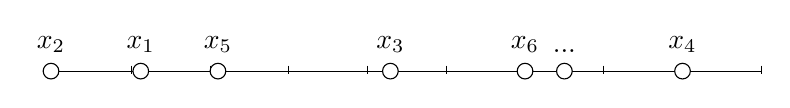
\begin{tikzpicture}
% a straight line segment
\draw (1,0) -- (10,0);
\foreach \x  in {1,...,10}
  \draw[xshift=\x cm] (0pt,2pt) -- (0pt,-1pt);
% the labels
\node[fill=white,draw=black,circle,inner sep=2pt,label=above:{$x_1$}] at (2.12,0) {};
\node[fill=white,draw=black,circle,inner sep=2pt,label=above:{$x_2$}] at (0.98,0) {};
\node[fill=white,draw=black,circle,inner sep=2pt,label=above:{$x_3$}] at (5.29,0) {};
\node[fill=white,draw=black,circle,inner sep=2pt,label=above:{$x_4$}] at (9,0) {};
\node[fill=white,draw=black,circle,inner sep=2pt,label=above:{$x_5$}] at (3.1,0) {};
\node[fill=white,draw=black,circle,inner sep=2pt,label=above:{$x_6$}] at (7,0) {};
\node[fill=white,draw=black,circle,inner sep=2pt,label=above:{...}] at (7.5,0) {};
\end{tikzpicture}
\end{center}

Escogemos el primer elemento $g_1$ de nuestra subsubcesión, y dividimos por la mitad el segmento.

\begin{center}
\begin{tikzpicture}
\draw (1,0) -- (10,0);
\foreach \x  in {1,...,10}
  \draw[xshift=\x cm] (0pt,2pt) -- (0pt,-1pt);
% the labels
\node[fill=black,draw=black,circle,inner sep=2pt,label=above:{$x_1$},label=below:{$g_1$}] at (2.12,0) {};
\node[fill=white,draw=black,circle,inner sep=2pt,label=above:{$x_2$}] at (0.98,0) {};
\node[fill=white,draw=black,circle,inner sep=2pt,label=above:{$x_3$}] at (5.29,0) {};
\node[fill=white,draw=black,circle,inner sep=2pt,label=above:{$x_4$}] at (9,0) {};
\node[fill=white,draw=black,circle,inner sep=2pt,label=above:{$x_5$}] at (3.1,0) {};
\node[fill=white,draw=black,circle,inner sep=2pt,label=above:{$x_6$}] at (7,0) {};
\node[fill=white,draw=black,circle,inner sep=2pt,label=above:{...}] at (7.5,0) {};

\draw[draw=red,ultra thick] (5.5,-1) -- (5.5,1);
\node[text=red] at (5.5,-1.3) {1};
\end{tikzpicture}
\end{center}

En al menos una de las dos mitades del segmento habrá infinitos términos: cogemos esa mitad y repetimos los mismos pasos. Finalmente, llegaremos a una subsucesión de este estilo:

\begin{center}
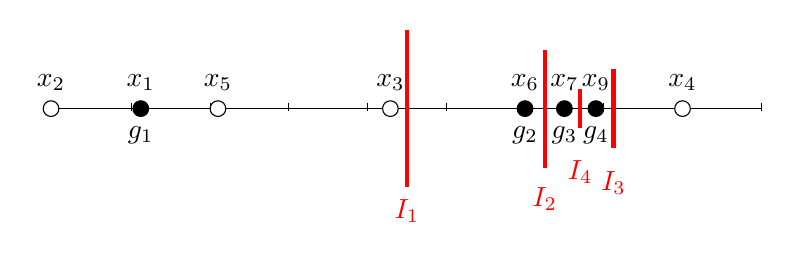
\begin{tikzpicture}
\draw (1,0) -- (10,0);
\foreach \x  in {1,...,10}
  \draw[xshift=\x cm] (0pt,2pt) -- (0pt,-1pt);
% the labels
\node[fill=black,draw=black,circle,inner sep=2pt,label=above:{$x_1$},label=below:{$g_1$}] at (2.12,0) {};
\node[fill=white,draw=black,circle,inner sep=2pt,label=above:{$x_2$}] at (0.98,0) {};
\node[fill=white,draw=black,circle,inner sep=2pt,label=above:{$x_3$}] at (5.29,0) {};
\node[fill=white,draw=black,circle,inner sep=2pt,label=above:{$x_4$}] at (9,0) {};
\node[fill=white,draw=black,circle,inner sep=2pt,label=above:{$x_5$}] at (3.1,0) {};
\node[fill=black,draw=black,circle,inner sep=2pt,label=above:{$x_6$},label=below:{$g_2$}] at (7,0) {};
\node[fill=black,draw=black,circle,inner sep=2pt,label=above:{$x_7$},label=below:{$g_3$}] at (7.5,0) {};
\node[fill=black,draw=black,circle,inner sep=2pt,label=above:{$x_9$},label=below:{$g_4$}] at (7.9,0) {};
\draw[draw=red,ultra thick] (5.5,-1) -- (5.5,1);
\node[text=red] at (5.5,-1.3) {$I_1$};

\draw[draw=red,ultra thick] (7.25,-0.75) -- (7.25,0.75);
\node[text=red] at (7.25,-1.15) {$I_2$};

\draw[draw=red,ultra thick] (8.125,-0.5) -- (8.125,0.5);
\node[text=red] at (8.125,-0.95) {$I_3$};

\draw[draw=red,ultra thick] (7.7,-0.25) -- (7.7,0.25);
\node[text=red] at (7.7,-0.8) {$I_4$};
\end{tikzpicture}
\end{center}

Nuestra subsucesión $\{g_x\}$ es igualmente infinita. Tal y como la hemos definido, tenemos que cada $g_i$ está en un intervalo $(I_i, I_{i-1})$ que cada vez se hace más pequeño. Es decir, que la subsucesión $\{g_x\}$ es de Cauchy y, por lo tanto convergente.

Ahora sólo queda ver cómo podríamos obtener esa subsucesión cuando estamos en espacios que no sean $\real^N$. La idea es sencilla: primero, buscamos una subsucesión que converja en la primera coordenada. Dentro de esa subsucesión, buscamos otra subsucesión que converja además en la segunda, y así con las $N$ coordenadas. 
\end{proof}

\begin{theorem} \label{thmCompactoMax} Sea $K\subset \real$ un conjunto compacto. Entonces, si $\appl{f}{\real}{\real}$ es continua en $K$ existen  $x_m,x_M \in K \tq F(x_m) \leq F(x) \leq F(x_M)\;\forall x \in K$.

Es decir, si $F$ es continua en $K$ alcanza su máximo y su mínimo en el conjunto.
\end{theorem}

\paragraph{Aplicación:}
$F(\gor{x}) = |||\gor{x}|||$ una norma (que ya sabemos que es continua):

\emph{Conclusión:} $m \md{x} \leq |||\gor{x}||| \leq C||\gor{x}||$

\begin{theorem}
En $\real^N$ TODAS las normas son equivalentes. 
\end{theorem}

\subsubsection{Conexión}
\begin{defn}[Conexión\IS por caminos]
Dados $a,b \in C$ podemos encontrar una aplicación continua $\appl{\varphi}{[0,1]}{\real^N}$ tal que $\varphi(0) = a$ y  $\varphi(1) = b$ con $ \varphi(t) \in C\, \forall t \in [0,1]$. 

Es decir, $C$ es conexo por caminos si podemos encontrar una "línea", un camino que una dos puntos cualquiera del conjunto y que además no se salga del conjunto.
\end{defn}

\begin{defn}[Conexión\IS por abiertos]
$C$ es conexo por conjuntos si para cualquier par de abiertos $A,B \subset \real^N \tq C\subset A\cup B$ se cumple que, si $A\cap C\neq \emptyset \y B\cap C \neq \emptyset $ entonces $ A\cap B \neq \emptyset$.

Esto es equivalente a decir que $C$ no puede ser expresado como unión de dos conjuntos disjuntos.
\end{defn}


\begin{remark}

\begin{figure}[hbtp]
\label{imgPeine}
\begin{center}
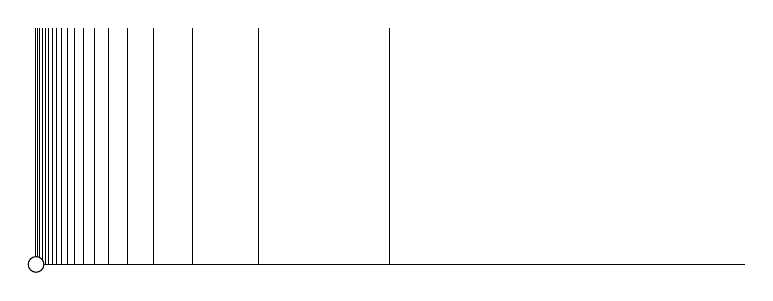
\begin{tikzpicture}

\draw (1,0) -- (10,0);

\foreach \x  in {2,...,20}
  \draw ($10/\x*(1,0) + (0.49,0)$) -- ($(0.49,3) + 10/\x*(1,0)$);

\node[fill=white,draw=black,circle,inner sep=2pt] at (1,0) {};

\end{tikzpicture}
\caption{Conjunto peine}
\end{center}
\end{figure}

Es curioso comprobar que estas 2 definiciones no son equivalentes. Tomemos el conjunto peine (figura \ref{imgPeine})
\[ \left\{(x,0), x\in (0,1]\right\} \cup \{(0,y), y \in (0,1]\} \cup \left\{\bigcup_{n=1}^{\infty}{\left(\frac{1}{n},y\right), y \in [0,1]}\right\} \]

Es un conjunto conexo por abiertos porque no podemos separarlo en dos conjuntos disjuntos. Sin embargo, no es conexo por caminos porque, si queremos ir del punto $(0,1)$ al $(0,0.5)$ no podemos hacerlo ya que el único camino pasaría por el punto $(0,0)$, que no está en el conjunto.
\end{remark}

\subsection{Funciones continuas, abiertos y cerrados}
 
 Al tener definida una norma de vectores podemos definir convergencia y continuidad:

\begin{defn}[Convergencia] Se dice que $\gx_n$ converge a $\gx$ (notación: $\gx_n \to \gx$) si

\[  \forall \varepsilon > 0\; \exists n_0 \tq n > n_0 \implies \md{\gx-\gor{x}_n}<\varepsilon \]

\end{defn}

\begin{defn}[Función\IS continua] Sea $\appl{F}{\real^N}{\real^M}$. Se dice que $F$ es continua en $a$ si y sólo si 

\[  \forall \varepsilon > 0 , \exists \delta > 0 \tq \md{\gx-\ga}_a < \delta \Rightarrow \md{F(\gx)-F(\ga)}_b< \varepsilon \]
\label{dfnContinua}
\end{defn}

\begin{remark} Es interesante ver que se puede hablar de continuidad tomando una norma en $\mathbb{R}^N$ y otra distinta en $\real^M$ sin por ello variar la definición de continuidad, teniendo en cuenta que todas las normas son equivalentes. \end{remark}

A partir de esta definición podemos estudiar qué hacen las funciones continuas con conjuntos abiertos y cerrados. Sea $F$ continua. Contrario a lo que podríamos intuir, 

\begin{enumerate}
\item A abierto no implica que  $F(A)$ sea abierto.
\item B cerrado no implica que $F(B)$ sea cerrado.
\end{enumerate}

Empezamos definiendo en qué consiste una función inversa:

\begin{defn}[Función\IS inversa] Dada \[\appl{F}{\real^N}{\real^N}\], definimos su inversa como
\[ \inv{F}(A) = \left\{\gor{x}\in \real^N \tq F(\gor{x})\in A\right\} \]
\end{defn}

A partir de aquí podemos extraer dos conclusiones que sí nos ayudarán a discernir si un conjunto imagen es abierto y cerrado.

\begin{theorem}[Función\IS inversa]\par\noindent\par
\label{thmInversa}
\begin{itemize}
\item F continua y A abierto $\implies F^{-1} (A)$ abierto.
\item F continua y B cerrado $\implies F^{-1} (A)$ cerrado.
\end{itemize}
\end{theorem}

Este teorema nos sirve para decir fácilmente si un conjunto es abierto o cerrado. Por ejemplo, consideremos
 \[ M=\{(x,y,z) \in \real^3 \tq x^2 + \cos\left(x\abs{y}\right) - e^z < 1 \} \]

Podemos definir ahí la función $F$ como 
\[ F(x,y,z) = x^2 + \cos\left(x\abs{y}\right) - e^z\]

que va de $\real^3$ a cierto conjunto $A = \{ a \in \real \tq a < 1 \}$. Podemos reescribir $M$ como
\[M=\{(x,y,z) \in \real^3 \tq  F(x,y,z) \in A\}\]

o, de otra forma, $M = \inv{F}(A)$. Según el teorema (\ref{thmInversa}), como $A$ es abierto entonces $M$ también es abierto.

\begin{proof} Demostramos las dos implicaciones que hemos enunciado.

1) Dado un $\gor{x} \in F^{-1} (A)$ queremos hallar un $R>0$ tal que $B_R(\gor{x})\subset F^{-1} (A)$. Partimos de 
\[\gor{x}\in F^{-1} (A) \dimplies F(\gor{x})\in A\]

Como $F$ es continua, $\exists \varepsilon>0 \tq B_{\varepsilon}(F(\gor{x}))\subset A$. Esto es equivalente a decir que, para cualquier $\gz$
\[ ||\gor{z}-F(\gor{x})|| < \varepsilon \implies \gor{z}\in A\]

Por la definición de continuidad (\ref{dfnContinua}), dado un $\gor{s}\in B_R(\gor{x})$ 

\[ \exists \delta > 0 \tq ||\gor{x}-\gor{s}||<\delta \implies ||F(\gor{x})-F(\gor{s})||< \varepsilon \]


y por lo tanto $F(\gor{s}) \in A$ y $\gor{s} \in F^{-1} (A)$.
Conclusión: Hemos encontrado un $\delta > 0$ tal que $s \in B_R(\gor{x}) \implies s \in F^{-1} (A)$.
\end{proof}

\section{Aplicaciones lineales y matrices}

\subsection{Aplicaciones lineales}

\begin{defn}[Aplicación\IS lineal]

Sea: $\appl{L}{\real^N}{\real^M}$. Entonces, $L$ es lineal si y sólo si

\[ L(\lambda \gor{x}) = \lambda L(\gor{x}) \] 
\[ L(\gor{x}+\gor{y}) = L(\gx)+L(\gy)\] 

\end{defn}
Además, toda aplicación lineal se puede escribir en forma de matriz.

\[L(\gor{x})=A\gor{x} =
\begin{pmatrix}
a_{11} 	& \cdots & a_{1n}		\\
\vdots	& \ddots &  \vdots 	\\
a_{n1}	& \cdots & a_{nn} 
\end{pmatrix}\]

\begin{theorem}
Toda aplicación lineal $L$ es continua.
\end{theorem}
\begin{proof} Partiendo de la definición de continuidad (\ref{dfnContinua}), $L$ es continua si y sólo si

\[ \forall \ga, \gx \; \forall \epsilon > 0 \; \exists \delta > 0 \tq \md{\ga - \gx} < \delta \implies \md{L\ga - L\gx} < \epsilon \]

Sabemos que $\md{A\gx} ≤ C\md{\gx}$ para alguna constante $C$. Podemos reescribir

\[ \md{L\ga - L\gx} = \md{L(\ga-\gx)} ≤ C\md{\ga-\gx} \]

Entonces, la igualdad se cumple si tomamos $\epsilon = C\delta$.
\end{proof}

\subsection{Norma de matrices}
Consideramos una aplicación continua

\begin{align*}
\appl{F}{\real^N&}{\real} \\
\gor{x} &\longrightarrow F(\gx) = \underbrace{||A\gx||}_{L(\gx)}
\end{align*}

Sabemos que existe $C>0$ tal que $||A\gx|| \leq C||\gx||$, es decir,  $||A\gx||\leq C$ si $||\gx||=1$. Queremos saber cuál es la mejor constante que podemos encontrar, la que más se ajuste. Consideramos el conjunto $M$ de todos los vectores de la esfera unidad, es decir 

\[ M = \{||A\gx|| \tq ||\gx||=1\}\subset \real \]

Entonces mejor constante $C$ es la cota superior mínima (supremo) que vamos a llamar $\alpha$. Al ser $F$ continua y $M$ compacto, sabemos que el supremo $\alpha \in M$.

\begin{defn}[Norma\IS de una matriz]
$$\norm{A} = \alpha = \max{\norm{A\gx} \tq \norm{\gx} =1}$$
\end{defn}

\begin{proof} Hay que demostrar que esta norma que hemos definido cumple las propiedades de una norma (\ref{defnNorma}). Las dos primeras son triviales, demostremos la desigualdad triangular
\[ \norm{A+B} = \max{\norm{(A+B)\gx}} = \norm{(A+B)\gx_{A,B}} \] 

donde $\gx_{A,B}$ es el vector que da el valor máximo para esa multiplicación. Usando la propiedad asociativa

\[  \norm{(A+B)\gx_{A,B}} = \norm{A\gx_{AB} + B\gx_{A,B}} ≤ \norm{A\gx_{A,B}} + \norm{B\gx_{A,B}} \]

Sabemos que existen dos vectores $\gx_A$ y $\gx_B$ que maximizan el resultado $\norm{A\gx_A}$ y $\norm{A\gx_B}$ respectivamente, por lo tanto

\[ \norm{A\gx_{A,B}} + \norm{B\gx_{A,B}} ≤ \norm{A\gx_A} + \norm{B\gx_B} = \norm{A} + \norm{B} \]

\end{proof}

Basándonos en lo que hemos obtenido, calculamos la norma uno de 
\[A = \begin{pmatrix}
      1&2\\-3&1\\2&0
     \end{pmatrix}\]  

Tenemos que maximizar, sabiendo que $|x|+|y| = 1$:

\[ |x+2y| + |-3x+y| + |2x| \leq |x|+|2y| + |3x| + |y| + 2|x| = 6|x|+3|y| \leq 6 (|x|+|y|) =6 \]
¿Podemos encontrar un vector $\gx = (x_0,y_0)$ tal que $||A(x_0,y_0)^T||_1 = 6$?\\
Tomando $x_0 = 1$ y $y_0 = 0$ lo encontramos. Como $\gx$ está en la esfera unidad y es una cota, es el máximo y por lo tanto la norma que buscamos.

Curiosamente, \textbf{coincide con la suma de los valores absolutos de las columnas} y escoger el más grande.

Si tomamos la norma infinito de 
\[A = \begin{pmatrix}
      1&2\\-3&1\\2&0
     \end{pmatrix}\]

Tenemos que \textbf{coincide con el máximo de las posibles sumas de los valores absolutos de las filas}.



Queremos buscar ahora cuánto vale la norma de una matriz cuando usamos la norma euclídea. Usaremos los dos lemas siguientes para apoyarnos.

\begin{lemma}
 Sea A una matriz cualquiera, entonces $\trans{A}A$ es simétrica.
\end{lemma}
\begin{lemma}
 \[ \underbrace{\pesc{\gx,A\gy}}_{\text{Producto en } \real^n} = \underbrace{\pesc{A^T \gx,\gy}}_{\text{Producto en } \real^M} \]
\end{lemma}

Tenemos $A^TA$ diagonalizable, de dimensión $N \times N$. Buscamos cuánto vale $\norm{A\gx}$ con  $\gx \in \real^N$. Empezamos desarrollando el vector en una base ortonormal de  $A^T A$: \[ \gx = \sum \alpha_i \gv_i \] y por lo tanto \[ ||\gx|| = \sum \alpha_i^2 \pesc{\gv_i,\gv_i}\].
 
 Desarrollamos el producto \[\trans{A}A\gx = \trans{A}A\left(\sum \alpha_i \gv_i\right) = \sum \left(\alpha_i\lambda_i\gor{v}_i\right) \] donde $\lambda_i$ son los autovalores de $\trans{A}A$. 
 
 Ahora queremos hallar el máximo de $||A\gx||$ cuando $||\gx|| = 1$:
 
 \[ ||A\gx||^2 = \pesc{A\gx,A\gx} = \pesc{\trans{A}A\gx,\gx} = \pesc{\sum \lambda_i \alpha_i \gv_i,\sum\alpha_i \gv_i} \]
 
 Como la base de $\{\gv_n\}$ es ortonormal, $\pesc{\gv_i, \gv_j} = 0$ si $i≠j$, por lo tanto sólo nos queda
 \[ \pesc{\sum \lambda_i \alpha_i \gv_i,\sum\alpha_i \gv_i} = \sum \lambda_i \alpha_i^2 \leq \lambda_{max} \left(\sum \alpha_i^2\right) = \lambda_{max} \]
 
 teniendo en cuenta que $\norm{\gx} = 1$ y donde $\lambda_max$ es el autovalor máximo. Es decir, hemos llegado a que
 \[ \max\norm{A\gx} ≤ \sqrt{\lambda_{max}} \]
 
 Hemos definido una cota para $\norm{A\gx}$. Ahora bien, esa cota se alcanza cuando $\gx$ es el autovector asociado a $\lambda_{max}$, por lo tanto la cota es un máximo y la norma de la matriz.
 
 \section{Límites}
 
 \begin{defn}[Límite] Dada una función $\appl{F}{\real^N}{\real^M}$, definimos su límite cuando $\gx\to\ga$ de la siguiente forma:
  \[ \lim_{\gx \rightarrow \ga} F(\gx) = \gor{L} \dimplies \forall \varepsilon > 0,  \exists \delta>0 \tlq 0<||\gx-\ga|| <\delta \implies ||F(\gx) - L||<\varepsilon\] 
 \end{defn}
 
 Importante el detalle de $0 < ||\gx-\ga||$, no es un $\leq$, porque no se necesita que la función esté siquiera definida en el punto $\ga$.  
 
 \begin{theorem}[Convergencia\IS de coordenadas]
  
  Sean $\gor{x}_n = (x_1,...,x_n) \in \real^N$ y $\gor{L} = (L_1,...,L_n) \in \real^N$. Entonces
 
  \[ x_n \rightarrow \gor{L} \dimplies (x_1 \rightarrow L_1) \y (x_2 \rightarrow L_2) \y ... \y (x_n \rightarrow L_n) \]
 \end{theorem}
 
 Idea para el cálculo de límites: 
 \begin{itemize}
  \item $\displaystyle\mylim{x}{a}{x} = \lim_{\gy\rightarrow 0} F(\gy+\ga)$.
  \item Límite a lo largo de rectas. $\displaystyle\mylim{x}{a}{\gx} \sim \lim F({t\gor{v}})$
 
 \end{itemize}
 
 Si $\displaystyle\lim F({t\gor{v}})$ toma valores distintos dependiendo de $\gor{v}$ entonces $\nexists \displaystyle\mylim{x}{0}{\gx}$
 
Por otra parte, si $\forall t \in \real, \mylim{x}{a}{t\gor{v}} = L$, entonces $\gor{L}$ es el candidato a ser el límite (no tiene por qué serlo). El siguiente paso sería demostrar con argumentos de comparación (Sandwich) u otros que $\mylim{x}{a}{\gx} = L$.
 
 El contraejemplo para ver que la existencia del límite por rectas no implica la existencia del límite es estudiar la función \[ f(x,y) = \frac{x y^2}{x^2 + y^4}\] . Veamos por qué.
 
 Si os acercamos al límite por medio de rectas:

 \[ f(x,y) = f(x,mx) = \frac{x\cdot(mx)^2}{x^2 + (mx)^4} = \frac{m^2x^3}{(1 + x^2m^4)x^2} \]
 \[ \lim{x\to 0} (f(x,mx)) \rightarrow 0, \forall m \in \real \]

 Pero si nos acercamos al límite por medio de $x = y^2$ tenemos:

\[ f(x,y) = f(y^2,y) = \frac{y^2y^2}{y^4+y^4} = \frac{y^4}{2y^4} = \frac{1}{2} ≠ 0\]  

Por lo tanto, el límite no existe a pesar de que existe cuando nos acercamos por rectas.
 
 
\begin{theorem}
 $F$ es continua si y sólo si para cualquier abierto $A$, $F^{-1}(A)$ es abierto.
\end{theorem}

\begin{proof}
De este teorema ya teníamos demostrada la implicación a la derecha (\ref{thmInversa}), así que sólo falta demostrar hacia la izquierda. Queremos probar que

\[ \forall \varepsilon > 0\; \exists \delta>0 \tlq ||\gx-\ga||<\delta \implies ||F(\gx)-F(\ga)||<\epsilon \]

Tomamos  \[ A = B_{\varepsilon}(F(\ga))\] de tal forma que \[ F(\ga) \in A \implies \ga \in F^{-1}(A) \]

Por hipótesis, $F^{-1}(A)$ abierto y $\ga \in F^{-1}(A)$ . Entonces 
\[\exists B_{\delta}(\ga) \subset F^{-1}(A) \].Es decir, \[ \gor{s}\in B_{\delta}(\ga) \subset F^{-1}(A), s\in F^{-1}(A) \implies F(s) \in A = B_{\varepsilon}(F(\ga))\]
\end{proof}

\begin{remark}
Este teorema también se cumple para cerrados.
\end{remark}

\section{Diferenciación}

\begin{defn}[Función\IS diferenciable]
 $F$ es diferenciable en $\gor{a}$ si existe una aplicación lineal $L$ tal que
 
\[ \frac{F(\gx)-F(\ga)-L(\gx-\ga)}{||\gx-\ga||} \convs[][\gx][\ga] 0 \]

que se puede expresar como
\[ \lim_{\gor{h} \rightarrow \gor{0}} \frac{\md{F(\ga+\gor{h}) - F(\ga) - L\gor{h}}}{||\gor{h}||} = 0 \]
\end{defn}

\begin{defn}[Diferencial]
A esa matrix $L$ la vamos a llamar la diferencial de $F$ en $\ga$:

\[ L\equiv DF(\ga) \]
\end{defn}

\begin{theorem} 
$$F \text{ diferenciable en } \ga \implies F \text{ continua en } \ga$$
\end{theorem}

\begin{proof}
 $$\lim_{\gor{h} \rightarrow \gor{0}} \frac{\md{F(\ga+\gor{h}) - F(\ga) - L\gor{h}}}{\md{\gor{h}}} = 0$$
 Esta es la definición de diferenciable. Para que este límite sea 0, el numerador tiene que tender a 0, por lo que $F(\ga+\gor{h}) - F(\ga) \rightarrow 0$
\end{proof}


\begin{theorem} 
Si la diferencial existe, entonces es única.
\end{theorem}

\begin{proof}  Vamos a demostrar que esa aplicación $L$ es única. Supongamos que existen $L_1,L_2$ que cumplen las condiciones.
\[0=\lim_{\gor{h} \rightarrow \gor{0}} \frac{F(\gor{a}+\gor{h}) - F(\ga)-L_1\gor{h}}{||\gor{h}||} = \lim_{\gor{h} \rightarrow \gor{0}} \frac{F(\gor{a}+\gor{h}) - F(\ga)-L_2\gor{h}}{||\gor{h}||}\].

Sumando:

\[ 0 = \lim_{\gor{h} \rightarrow \gor{0}} \frac{||F(\gor{a}+\gor{h}) - F(\ga)-L_1\gor{h}|| + ||F(\gor{a}+\gor{h}) - F(\ga) -L_2\gor{h}||}{||\gor{h}||} \]

Teniendo en cuenta que $||A-B|| = ||A+(-B)|| \leq ||A||+||B||$

\[ 0 \leq \lim_{\gor{h} \rightarrow \gor{0}} \frac{2\cdot\md{F(\ga + \gor{h}) - F(\ga)} + \md{L_1\gor{h}} + \md{L_2\gor{h}}}{\md{\gor{h}}} \]

\textit{Aquí falta completar.}
\end{proof}



\paragraph{Nomenclatura: }
Aproximación lineal $\sim$ Diferencial.

Matriz jacobiana $\sim$ Jacobiana.

\begin{defn}[Matriz\IS diferencial]
 Matriz asociada a $DF(\ga) \equiv $ Matriz de las derivadas parciales de F.
 
 $$DF(\ga) \equiv \begin{pmatrix}
                \dpa{F_1}{x_1} & \cdot & \dpa{F_1}{x_N}\\
                \vdots& \ddots & \vdots\\
                \dpa{F_N}{x_1} & \cdot & \dpa{F_N}{x_N}
                \end{pmatrix}
$$
\end{defn}

\begin{theorem}
 $F$ diferenciable en $\ga \implies \exists \deriv{F_k}{x_i}(\ga), i=1,2,...,N \y k = 1,2,...,M$
\end{theorem}

El contraejemplo para demostrar la implicación a la izquierda es el mismo que en los límites a lo largo de rectas.

$f(x,y) = \left\{ \begin{matrix}

\frac{xy^2}{x+y^2} & (x,y) = (0,0) \\ 
0 & (x,y)=(0,0)
           
          \end{matrix}\right.
$

Según las aplicaciones que tengamos, la diferencial se suele llamar de una u otra forma. Con $\appl{\delta}{\real}{\real^M}$ utilizamos notación vectorial en vez de matricial porque tendríamos una matriz columna. Por ejemplo: la velocidad (en un instante de tiempo, un punto en el espacio).

\begin{defn}[Gradiente] Sea $\appl{F}{\real^N}{\real}$, entonces definimos el vector gradiente como 

\[ \grad F(\gx) = DF(\gx) = \left(\dpa{F}{x_1}, \dpa{F}{x_2},\dotsc, \dpa{F}{x_n}\right) \]
\end{defn}


\subsection{Regla de la cadena}
\index{Regla!de la cadena}
Consideremos la composición de dos funciones de la siguiente forma:

$\appl{F}{\real^N}{\real^M}$. 

$\appl{G}{\real^M}{\real^K}$.

$\appl{H=G\circ F}{\real^N}{\real^K}$.

$ \gx \in \real^N, \gy \in \real^M$

\begin{wrapfigure}{r}{0.3\textwidth}
\begin{center}
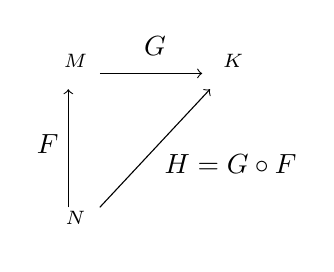
\begin{tikzpicture}
\draw[->] (-0.1,0.2) -- (-0.1,1.7);
\draw[->] (0.3,1.9) -- (1.6,1.9);
\draw[->] (0.3,0.2) -- (1.7,1.7);

\node at (0,0) {$\real^N$};
\node at (0,2) {$\real^M$};
\node at (2,2) {$\real^K$};

\node[left] at (-0.1,1) {$F$};
\node[above] at (1,2) {$G$};
\node[below right] at (1,1) {$H = G\circ F$};
\end{tikzpicture}
\end{center}
\caption{Composición de funciones}
\end{wrapfigure}

Con $F$ diferenciable en $\ga$ y $G$ diferenciable en $F(\gor{a})$. Entonces $H=G\circ F$ es diferenciable en $\ga $.
Además la expresión matricial es:

\[ \underbrace{DH(\ga)}_{K\times N} = \underbrace{DG(F(\ga))}_{K\times M}\cdot \underbrace{DF(\ga)}_{M\times N} \]
 
No hace falta calcular toda la matriz si sólo queremos un elemento. Para calcular 1 único elemento de la matriz diferencial (el de la fila $i$, columna $j$), usamos la siguiente fórmula
\[ \dpa{H_i}{x_j}(\ga) = \sum_{k=1}^M \dpa{G_i}{y_k}\cdot\dpa{F_k}{x_j} \]

Siempre teniendo en cuenta que $\displaystyle\dpa{G_i}{y_k}$ está evaluado en $F(\ga)$ y $\displaystyle\dpa{F_k}{x_j}$ está evaluado en $\ga$.

\subsection{Extensiones del Teorema del Valor Medio}

El teorema anterior que vimos del valor medio era para funciones de una variable, y proponía lo siguiente:
\begin{theorem}[Teorema\IS del valor medio (una variable)]
\label{thmTVM1var}
Dada $\appl{f}{\real}{\real}$ diferenciable, se tiene que \[ f(b)-f(a) = f'(c)(b-a)\] para algún $c\in[a,b]$
\end{theorem}

Después el teorema lo extendimos a funciones de $\real^N$ en $\real$: dada $\appl{F}{\real^N}{\real}$ entonces definíamos
 
 \[ \sigma(t)  = t\gor{b}+(1-t)\gor{a} \] 
 
 y $g = F\circ \sigma$ era una aplicación de los reales a los reales, y entonces aplicando el teorema anterior teníamos que 
 
 \[ F(\gor{b}-\gor{a}) = g(1)-g(0)  = g'(s) \] 
 para algún $s\in[0,1]$.

Sin embargo, al tratar de extrapolar este resultado a una función $\appl{F}{\real^N}{\real^2}$ nos queda que 

 \[ F(\gor{b})-F(\ga) = \begin{pmatrix}
                         \pesc{\nabla F_1(\gor{c_1}),{\gor{b}-\ga}}\\
                         \pesc{\nabla F_2(\gor{c_2}),\gor{b}-\ga}
                        \end{pmatrix}
 \]
  Tenemos 2 $c$ distintos, uno para cada $f$, por lo que este teorema pierde sentido. Hay que buscar una extensión, otra formulación del teorema que nos permita aplicarlo a las funciones que estamos estudiando.
  
  \begin{theorem} [Teorema\IS del valor medio (varias variables)]
  \label{thmTVM}
  Sea $f \in C^1$ en un abierto que contenga $[a,b]$. Entonces 
  
  \[ \norm{F(\gor{b})-F(\ga)} \leq \md{DF(\gor{c})} \cdot \md{\gor{b}-\ga} \]
  
  Siendo $c$ un punto del segmento que une $\ga$ y $\gb$ en el que $\md{DF(tb+(1-t)a)}$ alcanza su máximo.
  \end{theorem}  
  
  \begin{proof}

Primero vamos a demostrar la siguiente desigualdad:

\begin{equation}
\label{eqnTVM1}
 \md{\int_0^1 F(t) \,dt}≤ \int_0^1 \md{F(t)}\,dt 
\end{equation}

Si tomamos \[ L = \int_0^1 F(t) \,dt \]  entonces

\[ \md{L}^2 = \md{\int_0^1 F(t) \,dt}^2 = \pesc{L,\int_0^1 F(t) \,dt} \]

Como $L$ es un vector constante, podemos meterlo en la integral y tenemos que 

\[ \pesc{L,\int_0^1 F(t) \,dt} = \int_0^1 \pesc{L, F(t)} ≤ \int_0^1 \md{L}\md{F(t)} = \md{L} \int_0^1 \md{F(t)} \]

y por lo tanto

\begin{gather*}
\md{L}^2 ≤ \md{L} \int_0^1 \md{F(t)} \\
\md{L} ≤ \int_0^1 \md{F(t)} \\
\md{\int_0^1 F(t) \,dt } ≤ \int_0^1 \md{F(t)}  
\end{gather*}

quedando así demostrada la desigualdad (\ref{eqnTVM1}).

Consideramos ahora 

\[ \md{F(\gb) - F(\ga)} \]

Si integramos $DF$ por el camino que va de $\ga$ a $\gb$ nos queda que 

\[ \md{F(\gb) - F(\ga)} = \md{\int_0^1 DF\left[\ga(1-t) + t\gb\right](\gb - \ga)\, dt } \]

que por (\ref{eqnTVM1}) 

\[ \md{F(\gb)-F(\ga)} ≤ \int_0^1 \md{DF\left[\ga(1-t) + t\gb\right](\gb - \ga)}\, dt  \leq  \int_0^1 \md{DF\left[\ga(1-t) + t\gb\right]}\md{\gb - \ga}\, dt \]

Nos fijamos en $\md{DF\left[\ga(1-t) + t\gb\right]}$. Al ser continua y estar definida en un conjunto compacto, entonces alcanza su máximo en algún punto $\gor{c}$ entre $\ga$ y $\gb$, por lo tanto

\[ \md{F(\gb) - F(\ga)} ≤  \int_0^1 \md{DF(\gor{c})}\md{(\gb - \ga)} = \md{DF(\gor{c})}\md{\gb - \ga} \]
  \end{proof}

Este teorema nos sirve, por ejemplo, para ver que si tenemos $\appl{F}{\real^N}{\real^M}, F \in C^1$, definida en un conjunto abierto y conexo y  $DF(\gx) \equiv 0\; \forall\gx$, entonces $F$ es constante.

\subsection{Derivada direccional}

$\appl{F}{\real^N}{\real^M}$ (escalar)

$\ga \sim$ Recta que pasa por $\ga$ con dirección $\gor{v}$.

$r(t) = \ga + t\gor{v}$. 

\obs
Como una recta tiene infinitos vectores directores (dependiendo de la longitud), siempre tomaremos vectores directores unitarios, con $\norm{\gor{v}} = 1$.


Vamos a estudiar: $g(t) = F(\ga + t\gor{v}) = F \circ r (t)$.

$t \sim 0 \dimplies \ga + t\gor{v} \sim \ga$
\begin{defn} [Regla de la cadena]
$$g'(0) = \displaystyle\lim_{h \rightarrow 0} \frac{g(h)-g(0)}{h} = \displaystyle\lim_{h \rightarrow 0} \frac{F(\ga+h\gor{v})-F(\ga)}{h} \equiv D_{\gor{v}}F(\ga)$$. 
\end{defn}

\obs
La existencia de $D_{\gor{v}}F(\ga), \forall \gor{v}\in \real^N$ NO garantiza que $F$ sea derivable.


Si sabemos que $F$ SÍ es diferenciable podemos usar la regla de la cadena obteniendo:

$D_{\gor{v}}F(\ga) = g'(0) = D(F\circ r)(0) = ... = \pesc{\nabla F(\ga),\gor{v}}$


\paragraph{Aplicación:} 
\begin{itemize}
 \item 
 Dirección de máximo crecimiento:

$D_{\gor{v}}F(\ga) = \pesc{\nabla F(\ga),\gor{v}}\leq \norm{\nabla F(\ga)}\cdot \underbrace{\norm{\gor{v}}}_{\equiv 1}$

Conclusión:
\begin{align*}
D_{\gor{v}}F(\ga) &\leq \norm{\nabla F(\ga)}\\
&\uparrow\\
\text{El }= \text{se obtien}&\text{e cuando }\gor{v} = \displaystyle \frac{\nabla F(\ga)}{\norm{\nabla F(\ga)}}. 
\end{align*}

 
 \item
 Vector perpendicular a los conjuntos de nivel
 
 $\appl{F}{\real^N}{\real^M}$
 
 $S = \{ \gx \in \real^N \tq F(\gx) = 0\}$ (Conjunto de nivel)
 
 $\ga \in S$
 
 Entonces: $\nabla F(\ga) \perp S$
\end{itemize}

\begin{theorem}[Derivadas parciales continuas implican función diferenciable]
Si existen todas las derivadas parciales y son continuas $\implies F$ diferenciable en $\ga$.
 
\end{theorem}

Contraejemplo de la no reciprocidad: $f(x) = x^2 sin\left(\frac{1}{x}\right)$

\begin{proof}
 $\appl{F}{\real^2}{\real}$
 
 $$¿\frac{\left|F(a+a,b+k) - F(a,b) - \deriv{F}{x}(a,b) h - \deriv{F}{y}(a,b)k\right|}{\norm{(h,k)}}\longrightarrow 0?$$
 
 Sumamos y restamos al numerador $F(a,b+k)$.
 
 $$\frac{\left|\left(\underbrace{F(a+h,b+k) - F(a,b+k)}_{\deriv{F}{x}(a+\tilde{h},b+k) \text{ para algún } 0 \leq\tilde{h}\leq h} -  \deriv{F}{x}(a,b) h\right) + \left(\underbrace{F(a,b+k) - F(a,b)}_{\deriv{F}{x}(a+h,b+\tilde{k}) \text{ si } 0 \leq\tilde{k}\leq k}- \deriv{F}{y}(a,b) k\right)\right|}{\sqrt{h^2+k^2}}$$

 $$0\leq\frac{\left|\deriv{F}{x}(a+\tilde{h},b+k)-\deriv{F}{x}(a,b)\right| \cdot |h| + \left| \deriv{F}{y}(a,b+\tilde{k}) - \deriv{F}{y}(a,b)\right| \cdot |k|}{\sqrt{h^2+k^2}} = (*)$$
 
 Aquí es donde aplicamos que las derivadas parciales son continuas: como $h$ y $k$ son pequeños (por lo tanto $\tilde{h}<h$ también lo será) los puntos $(a,b)$ y $(a+h,b+k)$ también están cerca, por lo que sus imágenes por la derivada estarán también cerca, es decir, $|\deriv{F}{x}(a,b)-\deriv{F}{x}(a+\tilde{h},b+k)| \rightarrow 0$ y lo mismo con la otra.
 
 Conclusión:
 
 \begin{align*}
0 \leq (*) \leq \varepsilon \frac{|h|+|k|}{\sqrt{h^2+k^2}} &\leq C\varepsilon \rightarrow 0 \text{ cuando } \gor{h},\gor{k} \rightarrow \gor{0}\\
&\uparrow\\
\text{El numerdador es la} & \text{ norma 1 y el denominador la norma 2.}\\
\text{En } \real^N &\text{ todas las normas son equivalentes.}  
 \end{align*}
 
 
\end{proof}


\subsection{Derivadas iteradas}

\paragraph{Notación:}

$\deriv{}{y}\left(\deriv{f}{x}\right) \equiv \deriv{^2f}{x \partial y}$

\begin{theorem}[Euler (orden de las derivadas)]
Si las derivadas segundas son continuas, entonces:
$$\deriv{^2f}{x_i\partial x_j} = \deriv{^2 f}{x_j \partial x_i}$$
\end{theorem}

\subsection{Máximos y mínimos}

\begin{defn}[Máximo/mínimo\IS local] Sea $\appl{f}{\real^N}{\real}$. Diremos que $\vx_0 \in \real^N$ es un punto de máximo local si $\exists \epsilon > 0 \tq F(\vx_0) \geq F(\vx)\;\; \forall \vx \in B_{\epsilon} (\vx_0) $

La definición es análoga para el mínimo\end{defn}

\begin{remark} Por las propiedades del gradiente, si $F$ es diferenciable y $\vx_0$ es un máximo o mínimo local, entonces debe ser $\nabla F(\vx_0) = \vec{0}$.\end{remark}

\begin{defn}[Punto\IS crítico] $\vx \in \real^N$ es un punto crítico de $F$ si y sólo si $\nabla F(\vy) = \vec{0}$\end{defn}

No todos los puntos críticos son máximos o mínimos, así que tenemos que clasificarlos de alguna forma. Para ello, usamos el polinomio de Taylor de orden 2, de forma que 

\[F(x,y) = F(x_0, y_0) + \pesc{\nabla F(x_0, y_0), (x-x_0, y-y_0)} +\]\[\frac{1}{2}(x-x_0, y-y_0)\left(\begin{matrix} \frac{\partial^2 f}{∂ x^2} (x_0,y_0) & \frac{\partial^2 f}{\partial x \partial y} (x_0,y_0) 
\\ \frac{\partial^2 f}{\partial y \partial x} (x_0,y_0) & \frac{\partial^2 f}{\partial y^2} (x_0,y_0) \end{matrix}\right) \left(\begin{matrix} x - x_0 \\ y - y_0 \end{matrix}\right) + \epsilon \]

Simplificando nos queda que:

\[F(\vx) = F(\vx_0) + \pesc{\nabla F(\vx_0),\vx - \vx_0} + \frac{1}{2}(\vx - \vx_0) D^2F(\vx_0) (\vx - \vx_o) ^T + \epsilon\]

Dado que el gradiente es 0, el punto clave es el signo de $\frac{1}{2}(\vx - \vx_0) D^2F(\vx_0) (\vx - \vx_o) ^T$. Para ello, usamos las siguientes definiciones del álgebra lineal.

\subsubsection{Resultados de álgebra lineal}
\index{Matriz!semidefinida positiva/negativa}
\index{Matriz!definida positiva/negativa}
\begin{defn}[Matriz semidefinida y definida positiva y negativa][]\noindent\\ \indent
La matriz $A$ de dimensión $N\x N$ es semidefinida positiva si y sólo si $\vv A \vv^T \geq 0 \;\; \forall \vv \in \real^N$.

La matriz $A$ de dimensión $N\x N$ es definida positiva si y sólo si $\vv A \vv^T > 0 \;\; \forall \vv ≠0 \in \real^N$.

La matriz $A$ de dimensión $N\x N$ es semidefinida negativa si y sólo si $\vv A \vv^T \leq 0 \;\; \forall \vv \in \real^N$.

La matriz $A$ de dimensión $N\x N$ es definida negativa si y sólo si $\vv A \vv^T < 0 \;\; \forall \vv ≠0 \in \real^N$.
\end{defn}

\begin{theorem}
Si una matriz es simétrica, existe una base en la cual la matriz es diagonal.
\end{theorem}

\index{Autovalor}
\index{Autovector}
Sea $A$ una matriz $N\x N$. Entonces diremos que un vector $\vv ≠ \vec{0}$ es un autovector asociado al autovalor $\lambda\in \real$ si y sólo si $A\vv = \lambda\vv$. Dado que podemos escribir

\[ A = \left(\begin{matrix}
a & b \\ c &  d
\end{matrix}\right)\;\;\;\; \vv = \left(\begin{matrix}
x\\ y
\end{matrix}\right) \], entonces tenemos que $A\vv = \lambda \vv$ si y sólo si

\[ \left\lbrace\begin{matrix}ax+by=\lambda x \\ cx+dy = \lambda y \end{matrix}\right. \]

Es decir, la autorrecta $\begin{pmatrix} x \\ y \end{pmatrix}$ es una solución no trivial del sistema anterior. Sin embargo, para que haya soluciones no triviales el determinante de la matriz $\begin{pmatrix}a-\lambda & b \\ c & d - \lambda\end{pmatrix}$ debe ser 0.

Por lo tanto, los autovalores son las soluciones de la ecuación $det(A-\lambda I) = 0$, siendo $I$ la matriz identidad.

\begin{theorem}
Si un conjunto de autovectores es una base, entonces la matriz $A$ expresada respecto a esa base pasa a ser diagonal, y los elementos de la diagonal son los autovalores. 

Si dos autovalores son distintos, los autovectores asociados son distintos.

Si A es simétrica, entonces el conjunto de autovectores es una base.
\end{theorem}

Volvemos ahora al cálculo.

\begin{theorem}[Clasificación de puntos críticos][]
Sea $\appl{F}{\real^N}{\real}$, $F\in C^2$ (con dos derivadas continuas), y sea $\vx_0$ un punto crítico. Entonces

\begin{enumerate}
\index{Máximo/mínimo!local}
\index{Punto!de silla}
\index{Punto!crítico degenerado}

\item Si \textbf{todos} los autovalores de $D^2F(\vx_0)$ son \textbf{mayores que cero}, entonces $D^2F(\vx_0)$ es definida positiva y $\vx_0$ es un \textbf{mínimo local}.
\item Si \textbf{todos} los autovalores de $D^2F(\vx_0)$ son \textbf{menores que cero}, entonces $D^2F(\vx_0)$ es definida negativa y $\vx_0$ es un \textbf{máximo local}.
\item Si \textbf{algunos} autovalores son \textbf{mayores que cero} y otros son \textbf{menores que cero}, entonces $\vx_0$ es un \textbf{punto de silla.}
\item Si algún autovalor \textbf{es 0}, y el resto son mayores o menores que cero, entonces $\vx_0$ es un \textbf{punto crítico degenerado}.
\end{enumerate}
\end{theorem}

\subsubsection{Ejemplos}

Tomamos $F(x,y) = x^2 + y^2 +xy$. Obtenemos los puntos críticos, es decir, los puntos en los que $\nabla F(x,y) = (0,0)$. El punto resultante es $(0,0)$. Estudiamos el tipo de punto crítico. Para ello, calculamos la matriz hessiana en ese punto:

\[ D^2F(0,0) = \begin{pmatrix}2&1\\1&2\end{pmatrix}\]. 

Los autovalores son las soluciones de

\[ 0 = det\left(\begin{pmatrix}2&1\\1&2\end{pmatrix} - \lambda \begin{pmatrix}1&0\\0&1\end{pmatrix}\right) = det\begin{pmatrix}2-\lambda & 1 \\ 1 & 2-\lambda\end{pmatrix} = (2-\lambda)^2  - 1\]

Por lo tanto, $\lambda$ es $3$ o $1$. Dado que ambos autovalores son mayores que 0, entonces $D^2F$ es definida positiva y $(0,0)$ es un mínimo local.

\subsection{Máximos y mínimos absolutos}

\begin{defn}[Máximo/mínimo\IS absoluto] Sea $\appl{F}{\real^N}{\real}$ y $A\subset \real^N$. $\vx_m$ es un máximo absoluto de $F$ en $A$ si y sólo si $F(\vx_m) ≥ F(\vx)\;\; \forall \vx \in A$. La definición es análoga para el mínimo.
\end{defn}

\begin{theorem}[Teorema\IS de compacidad]
Tenemos un conjunto $K\subset \real^N$ compacto (cerrado y acotado). Supongamos la sucesión $\{\vx_n\}_{n\in\nat}\subset K$. Entonces podemos encontrar al menos una subsucesión $\{\vx_{n_j}\}_{j\in\nat} \subset \{\vx_n\}_{n\in\nat}$ tal que $\{\vx_{n_j}\}$ es convergente.
\end{theorem}

\begin{proof}
Trabajamos en dimensión 2, pero la demostración es análoga.
Como $K$ es compacto, podemos encontrar un cuadrado $Q_0$ de lado $L$ que encierre completamente a $K$. Divido $Q_0$ en $2^2$ cuadrados de lado $L/2$.  En alguno de ellos hay infinitos términos de la sucesión: lo llamamos $Q_1$ y me quedo con uno de los términos de la sucesión, al que llamamos $x_1$. Volvemos a dividir este cuadrado en cuatro cuadrados, elegimos uno que tenga infinitos términos de la sucesión y seleccionamos un elemento de la sucesión dentro al que llamamos $x_2$. Repetimos esto muchas veces, de forma que cada término $x_n$ está encerrado en el cuadrado $Q_n$ de lado $\frac{L}{2^n}$. 

Si $k,l > n$, entonces es claro que $\md{\vx_k-\vx_l}$ es menor o igual que la diagonal de $Q_n$, que es $\frac{L}{2^n}\sqrt{2}$, que tiende a cero cuando $n\to\infty$. Por el criterio de Cauchy, entonces esta sucesión es convergente, y como $K$ es cerrado el límite pertence a $K$.
\end{proof}

\begin{theorem}
Sea $K\subset \real^N$ compacto y $\appl{F}{\real^N}{\real}$, continua en $K$. Entonces, $F$ alcanza su máximo y mínimo absolutos en $K$.
\end{theorem}

\begin{proof}

Como $F$ es acotada, existe $\alpha = \sup \{ F(x) \tq x \in K\}$. Existe entonces una sucesión $\{x_n\}$ tal que si $n\to \infty$ entonces $F(x_n)\to \alpha$. 
Sabemos que existe $\{x_n\}\subset K$, por lo que existe una subsucesión$\{x_{n_j}\}$ convergente tal que $x_{n_j} \to x_0 \in K$

Como $F$ es continua, $F(x_{n_k})\to F(x_0)$, es decir $F(x_{n_j}) \to \alpha$, por lo tanto el supremo es el máximo.
\end{proof}

\subsubsection{Ejemplos}

La función a estudiar es $F(x,y) = x^2-y^2$ en la bola $\omega = \{ x^2 + y ^2 ≥ 1\}$. Es diferenciable en todo $\real$ porque es un poliniomio. 

Calculamos el diferencial y vemos qué ocurre cuando es 0 \[\nabla F = (2x, -2y) = (0,0) \implies (x,y) = (0,0)\]

Operando, vemos que el punto $(0,0)$ es un punto de silla. Ahora sólo queda ver el comportamiento en la frontera $C$, cuando $x^2+y^2 = 1$. $F$ restringida a $C$ quedaría de la siguiente forma:

\[ F(\cos t, \sin t) = \cos^2 t - \sin^2 t = \cos 2t\]

El coseno tiene máximos cuando $t=0$ y $t=\pi$, y mínimos cuando $t=\pi /2$ y $t=3\pi /2$. Es decir, tiene máximos absolutos en los puntos $(1,0),\;(-1,0)$ y mínimos absolutos en $(0, -1)$, $(0, 1)$. 

\begin{theorem}[Teorema\IS de los multiplicadores de Lagrange]
Tenemos una función $\appl{F}{\real^2}{\real}$ y una restricción $G(x_1,\cdots,x_n) = k$, resolvemos el siguiente sistema:

\begin{align*}
\nabla F &= \lambda \nabla G \\
G &= k
\end{align*} 

\end{theorem}


\section{Desarrollo de Taylor}
\index{Polinomio!de Taylor}
Tenemos una función $\appl{F}{\real^N}{\real}$, con $F\in C^k$ ($k$ veces derivable), y queremos el desarrollo de Taylor de $F$ alrededor de $\ga \in \real^N$.

En dimensión 1, el desarrollo era el que sigue

\[ g(x) = g(0) + g'(0)x + \frac{g''(0)}{2!}x^2 + ... + \frac{g^{k)}(0)}{k!}x^k + \underbrace{\frac{g^{k+1)}(s)}{(k+1)!}x^{(k+1)}}_{\text{error}} \]

Tenemos que expandir este desarrollo a más dimensiones. Tomamos \[ g(t) \equiv F(t(\ga + \gor{h}) + (1-t)\ga) \] reduciendo así el cálculo a dimensión 1. Operamos ahora para calcular las derivadas:

\begin{gather*}
g'(t) = \pesc{\nabla F(a+th),h} = \sum_{i=1}^N \deriv{F}{x_i}(a+th)\cdot h_i \\
g''(t) = \sum_{i=1}^N\left(\sum_{j=1}^N \deriv{}{x_j}\deriv{F}{x_i}(\ga+\gor{h})\cdot{h_j}\right)h_i = \sum_{i,j = 1}^N \deriv{^2F}{x_i \partial x_j}(\ga+t\gor{h})h_ih_j \\
\dotsb \\
\frac{g^{s)} (0)}{s!} = \frac{1}{s!}\sum_{i_1,i_2,...,i_s=1}^N \frac{\partial^s F}{\partial x_{i_1},x_{i_2},...,x_{i_s}}
\end{gather*}

De esta forma, el desarrollo de Taylor de orden $k$ de $F$ en $\ga$ en general es

\begin{equation}
T^k_F(x) = \sum_{\alpha = 0}^k 
	\left( 
		\frac{1}{\alpha !}
		\sum_{i_1,\dotsc,i_\alpha = 0}^N 
			(x_{i_1} - a_{i_1}) \dotsb (x_{i_\alpha} - a_{i_\alpha}) 
			\frac{\partial^\alpha F}{\partial x_{i_1} \dotsb \partial x_{i_\alpha}} 
			 (\ga)
	\right) 
\end{equation}

Por ejemplo, el desarrollo de Taylor de una función $F(x,y)$ con $\ga = (a,b)$ queda lo siguiente (con $F_{xyz\dotsc} = \dfrac{\partial^nF}{\partial x \partial y \partial z \dotsb}$)

\begin{align*}
T^k_{F}(\gx) &= F(\ga) \\
& +  (x - a) F_x(\ga) + (y - b) F_y(\ga)  \\
& +\frac{1}{2!}\left[(x-a)^2F_{xx}(\ga) + 2(x-a)(y-b)F_{xy}(\ga) + (y-b)^2F_{yy}(\ga)\right] \\
& +\frac{1}{3!}\left[(x-a)^3F_{xxx}(\ga) + 3(x-a)^2(y-b)F_{xxy}(\ga) + 3(x-a)(y-b)^2 F_{xyy} (\ga) + (y-b)^3F_{yyy} (\ga)\right] \\
& +\dotsb
\end{align*}

Existe una forma más compacta para el desarrollo de Taylor de orden dos usando el producto escalar, el vector gradiente y la matriz hessiana ($D^2F$) de derivadas segundas:

\[ F(\gor{a}+\gor{h}) = F(\ga) + \pesc{\grad F(\ga),\gor{h}} + \frac{1}{2} \gor{h}^T D^2F(\ga)\gor{h} \]

\begin{theorem}[Teorema\IS de Taylor]
 $$\frac{|F(\ga)+\gor{h} - P_{s,a}(\gor{h})|}{\norm{\gor{h}}^s} \rightarrow 0, \text{ Cuando } \gor{h} \rightarrow 0$$
 Además $P_{s,a}(\gor{h})$ es el único polinomio de orden S que hace que el límite sea 0.
\end{theorem}


\chapter{Teoremas de la función inversa y sus variantes}

\section{Teorema de la aplicación contractiva}

En el mundo lineal tenemos podemos resolver sistemas de dos formas. Con $\appl{F}{\real^N}{\real^N}$ y $L(\gx) = A\gx$, siendo $A$ una matriz $N\x N$; queremos resolver el sistema $A\gx = \gy$ sabiendo que $A\gor{0} = \gor{0}$.

Este sistema tiene solución si y sólo si  $\det(A) \neq 0$: es la condición para que exista $A^{-1}$.

Existe también la posibilidad de tener una función $\appl{F}{\real^{N+M}}{\real^N}$ con $L(\gx) = A\gx$, $A$ matriz $N\x (N+M)$.

Para resolver el sistema $A\gx = \gy$ parametrizamos $M$ variables.

En el mundo \textbf{no lineal}, consideramos una función $\appl{F}{\real^N}{\real^N}$. Entonces tenemos un sistema de ecuaciones

\[ \left.\begin{matrix}
F(x_1,\dotsc,x_N) = y_1\\
F(x_1,\dotsc,x_N) = y_2\\
\vdots\\
F(x_1,\cdots,x_N) = y_N          
        \end{matrix}
\right\} F(\gx)=\gy \]

Vamos a intentar resolver este problema utilizando Taylor para aproximar al orden lineal, pero tenemos que pagar un precio: para que taylor funcione tenemos que trabajar cerca del punto. Esto significa que \textbf{el resultado va a ser local}.


\begin{theorem}[Teorema\IS de la aplicación contractiva] Sea 
\begin{itemize}
\item $\appl{F}{\real^N}{\real^N}$ o
\item $\appl{F}{C}{C}, C\in \real^N$, cerrado, o
\item $\appl{F}{K}{K}, K\in \real^N$, compacto.
\end{itemize}

Supongamos que existe $\alpha\in(0,1)$ tal que

\[ \md{F(x)-F(y)}\leq \alpha\md{x-y} \forall x,y \in \left\{\begin{matrix}
                                                           \real^N\\
                                                           C\\
                                                           K
                                                          \end{matrix}\right. 
                                              \]
                                              
  Entonces                                          
                                           
\[  \exists ! x_0 \in\left\{\begin{matrix}         \real^N\\
                                                           C\\
                                                           K
                                                          \end{matrix}\right. 
                                                        \tlq F(x_0) = x_0 \text{ (Punto fijo)} \]
\label{thmAC}
\end{theorem}


\begin{proof} Primero llevamos los casos de $C$ y $\real^n$ a un conjunto compacto $K$. Partimos de 

\begin{equation}
\md{F(\gx) - F(\ga)} \leq \alpha\md{\gx-\ga} \label{eqAC_hip}
\end{equation} 

y veamos qué ocurre para un vector general $\gx$: \[ \md{F(\gx)} = \md{(F(\gx)-F(\ga)+F(\ga)} \leq \md{F(\gx)-F(\ga)} + \md{F(\ga)} \] 

Aplicando (\ref{eqAC_hip}) tenemos que 
\[\md{F(\gx)} ≤ \alpha \md{\gx-\ga} + \md{F(\ga)} \]
  
  Si tomamos $\ga=0$ (en el caso  $0 \notin C $ solo haría falta una pequeña traslación), y suponemos $ \md{x} < R$, tenemos entonces que \[ \md{F(\gx)} \leq \alpha R + \md{F(\gor{0})} < R\]
  Es decir, $F$ toma un compacto y lo lleva en sí mismo: $\appl{F}{B_R(0)}{B_R(0)}$. Podemos seguir la demostración ahora suponiendo que estamos trabajando siempre sobre un compacto.
  
  El siguiente paso es llevar a cabo un \textbf{proceso iterativo}. Tenemos \[ \appl{F}{K}{K} \] con  $K\subset \real^N$ conjunto compacto. Definimos entonces la sucesión de $\{x_n\}_{n \in \nat} \subset K$, construido de forma iterativa con $x_n = F(x_{n-1})$. Vamos a demostrar que esa sucesión es de Cauchy, lo que implicaría que es convergente.
  
 Para ello, dado $\epsilon > 0$ hay que hallar $n_0$ tal que si $n,m>n_0$ entonces $\md{x_n-x_m}<\epsilon$. Pongamos, para facilitar la demostración, que $n>m$. 
 
 Entonces, sumamos y restamos a ese módulo cada uno de los $x_i$ entre $n$ y $m$: 
 
 \begin{equation}
  \md{x_n - x_m} = \md{x_n \pm x_{n-1} \pm \dotsb \pm x_{m+1} - x_m} \leq \sum_{i=m}^n \md{x_i - x_{i-1}} \label{eqAC_sum}
 \end{equation}
 
Operamos ahora con cada uno de esos sumandos. Por ejemplo, con $i = n$, vemos que 

\begin{gather*}
\md{x_n - x_{n-1}} = \md{F(x_{n-1}) - F(x_{n-2})} \leq \alpha \md{x_{n-1} - x_{n-2}} = \\
= \alpha \md{F(x_{n-2}) - F(x_{n-3})} ≤ \alpha ^2 \md{x_{n-2}-x_{n-3}} 
\end{gather*}

Si seguimos operando, llegaremos a que $ \md{x_n - x_{n-1}} \leq \alpha^{n-2} \md{x_2-x_1}$. Generalizando, tenemos que

\[ \md{x_i - x_{i-1}} ≤ \alpha^{i-2} \md{x_2-x_1} \]

Aplicando esta fórmula en (\ref{eqAC_sum})
 
\[ \md{x_n-x_m} \leq \left(\alpha^{n-2} + \alpha^{n-3} + \dots + \alpha^{m-1}\right) \md{x_2 - x_1}\]

Esa suma de $\alpha$'s es la suma de una sucesión geométrica de razón $\alpha$. Por lo tanto, la podemos simplificar como \[\sum_{k=m-1}^{n-2} \alpha^k = \alpha^{m-1}\frac{1-\alpha^{n-m}}{1-\alpha} ≤ \frac{\alpha^{m-1}}{1-\alpha} \], y la ecuación nos queda de la forma \[ \frac{\alpha^{m-1}}{1-\alpha}  \md{x_2-x_1} \]. Dado que $\dfrac{\alpha^{m-1}}{1-\alpha}  \convs[][n_0] 0$, tendremos que tomando un $n_0$ suficientemente grande se cumple que 

\[ \frac{\alpha^{m-1}}{1-\alpha}  \md{x_2-x_1} < \varepsilon \]

para un $\epsilon$ arbitrariamente pequeño. Con esto \textbf{demostramos que la sucesión de $x_n$ es de Cauchy} y por lo tanto es convergente a un cierto límite $x_0$.

Tal y como habíamos construido la sucesión, tenemos que 

\begin{equation} \label{eqAC_suc}x_n= F(x_{n-1}) \end{equation}

$x_n$ converge a $x_0$ cuando $n\to\infty$. De la misma forma, como $x_{n-1}$ también converge a $x_0$, está claro que $F(x_{n-1})$ convergerá a $F(x_0)$. Sustituyendo estos dos resultados en (\ref{eqAC_suc}), tenemos que 

\[ x_0 = F(x_0) \]

Hemos demostrado por lo tanto que el límite de esa sucesión que hemos construido \textbf{es un punto fijo} de la función. 

Nos queda \textbf{demostrar ahora que ese punto es único}, y lo haremos por reducción al absurdo:

 Supongamos que existen dos puntos fijos:
 
 \begin{gather*}
 a = F(a)\\
 b= F(b)
\end{gather*}
                     
 Entonces tendríamos que \[ \md{a-b} = \md{F(a)-F(b)}\leq \alpha \md{a-b} \] pero como $\alpha$ es menor estricto que 1, entonces tendríamos que \[ \md{a-b} < \md{a-b} \], lo que es una contradicción.
\end{proof}

El teorema de la aplicación contractiva nos sirve, por ejemplo, para comprobar si hay una solución de una ecuación diferencial ordinaria (EDO).

$$\left.\begin{matrix}y'(x) = f(x,y(x))\\
        y(x_0) = y_0
       \end{matrix}\right\} \leftrightarrow y(x) = y_0 + \int_{x_0}^x f(s,y(s)) ds$$

Podemos definir:

\begin{align*}
y_1(x) &= y_0 + \int_{x_0}^{x} f(s,y_0)ds\\
y_2(x) &= y_0 + \int_{x_0}^x f(s,y_1(s))ds \equiv T(y_1)\\
&\dots\\
y_n &= T(y_{n-1}) =  y_0 + \int_{x_0}^x f(s,y_{n-1}(s))ds\\
¿T(y) &= y?
\end{align*}
Aquí es donde entraría la diferencia entre trabajar en $\real^N$ y un espacio de funciones.

Ejercicio propuesto: Aplicar este argumento a iterativo

$\left. \begin{matrix} y' = y\\
         y(0) = 1 \equiv y_0
        \end{matrix}\right\}$

        
\section{Teorema de la función inversa}
En Cálculo I teníamos el siguiente teorema:
\begin{theorem} Sea $\appl{f}{\real}{\real}\; f\in C^1$ y $f'(a) \neq 0$. Entonces $f$ es invertible en un entorno de $f(a)$. 

La inversa es diferenciable en ese entorno, y además $(f^{-1})'(f(a)) = \frac{1}{f'(a)}$
\end{theorem}

El teorema nos daba un resultado \textbf{local} que asegura que existe la inversa, que es diferenciable y además nos daba su fórmula. 

Buscamos ahora lo que ocurre en dimensión $N$. Tomamos $\appl{f}{\real^N}{\real^N}$ y supongamos que en algún abierto $\exists F^{-1}$ y $F,F^{-1} \in  C^1$.

Entonces está claro que

\[ (F\circ \F)(y) = y \implies DF(\F(y))D\F(y) = Id \]
\[ (\F\circ F)(y) = y \implies D\F(F(y))DF(y) = Id \]

Con $\appl{F}{\Omega\subset \real^N}{\real^N}$ queremos probar que existe una aplicación $\appl{G}{V}{U}$ que verifique las siguientes condiciones

\begin{gather*}
G\circ F(\gx) = \gx, \forall\gx\in U \subset \Omega \\
F\circ G(\gy) = \gy, \forall \gy \in V \\
G \text{ diferenciable}
\end{gather*}

\begin{theorem} [Teorema\IS de la función inversa]
\label{thmInv}
Sea $\appl{F}{\Omega\subset\real^N}{\real^N} \text{ con } F\in C^1(\Omega)$.

Supongamos $DF(\ga)$ invertible, $\ga \in \Omega$.

Entonces existe un abierto $V \tlq F(\ga)\in V$, un abierto $U \tlq \ga \in U$ y una inversa local $\appl{G}{V}{U}$.\\
Además, $G$ es diferenciable en $U$ y $DG(y) = \left[DF(\F(y))\right]^{-1}, \forall y \in U$.
\end{theorem}

\begin{proof} Haremos la demostración en varios pasos.

 \paragraph{1: Simplificar la notación}  Queremos invertir $F(x) = y, \gor{y} \sim F(\ga), \gx \sim \gor{a}$.
 
 Llamamos:
 \begin{itemize}
  \item $y = F(\ga) + \gor{z}; \gor{z} \sim \gor{0}$
  \item $y = \ga + \gor{s}; \gor{s} \sim \gor{0}$
\item  $F(\ga+\gor{s}) = F(\ga)+\gor{z}$.
  \end{itemize}
 Definimos además \[ \tilde{F}(\gor{s}) \equiv F(\ga + \gor{s}) - F(\ga) = \gor{z} \] de tal forma que  \[ \tilde{F}(\gor{0}) = \gor{0} \]
 
 Es decir, hacemos una traslación para suponer que $F(\gor{0}) = \gor{0}$.
 
 Por las hipótesis del teorema, sabemos que $\det DF(\gor{0}) \neq 0$
 
 Es claro que resolver para $F$ es exactamente lo mismo que resolver para $CF(\gx) = \gor{y}$, donde C es una matriz invertible.
 
 Tomamos $\tilde{F} = [DF(\gor{0})]^{-1}F$, de tal forma que ganamos la siguiente igualdad

 \[ D\tilde{F}(\gor{0}) = Id \]
 
 \paragraph{2: Formulación como punto fijo.}

 Partimos de $F(\gor{0})=\gor{0}$ y $ DF(\gor{0}) = Id$.
 
 Definimos $f(\gx) = \gx - F(\gx)+\gy$
 
 Entonces resolver $F(\gx) = \gor{y}$ es lo mismo que encontrar un punto fijo $f(\gx) = \gx$. Por lo tanto, ahora nuestro objetivo es probar que $f$ es contractiva para así poder aplicar el teorema de la aplicación contractiva (\ref{thmAC}).
 
 \paragraph{3: Estimar $f$} Empezamos con
 
 \[ Df(\gx) = Id - DF(\gx) \rightarrow Df(\gor{0}) = Id - DF(0) = Id - Id = \begin{pmatrix}  \bigzero \end{pmatrix}  \]
   
 La primera estimación que podemos hacer es sobre el determinante. Si $DF(\gor{0}) = Id$, entonces $\det(DF(\gor{0})) = 1$. Como $F$ es continua, entonces 
 
 \[ \exists \varepsilon_0 >0 \tlq \md{\gx} \leq \varepsilon_0 \implies  \det(DF(\gor{0}))>0 \]
 
  Es decir, en un entorno del $\gor{0}$, el determinante sigue siendo positivo.
  
  
 Ahora estimamos información sobre el diferencial de $f$. Como $F\in C^1$, entonces también se cumple que $f \in C^1$. Como $\appl{f}{\real^N}{\real^N}$, entonces
  
  \[ Df(\gor{0}) = \begin{pmatrix}
                  Df_1(\gor{0}) \rightarrow\\
                  \vdots\\
                  Df_N(\gor{0}) \rightarrow
                 \end{pmatrix} = \begin{pmatrix}  \bigzero \end{pmatrix} \]
                 
 Por tanto $\md{Df_i(\gor{0})} = 0$.
 
 Por continuidad $\exists \varepsilon_i > 0 \tlq \md{x} \leq \varepsilon_i, \implies \md{Df_i(\gx)} <\frac{1}{2N}$. Fijamos un $\varepsilon = \min \{\varepsilon_0,\varepsilon_1,\dotsc, \varepsilon_N\} ,\, i=0,\dotsc,N$.
 
 Entonces, si $\md{x} \leq \varepsilon$ tenemos  que
\begin{gather}
\det(DF(\gx))>0 \label{eqFinv_DetF} \\
\md{Df_i(\gx)}  = \md{\nabla f_i(\gx)} < \dfrac{1}{2N}, i=1,2,...,N \label{eqFinv_Detfi}
\end{gather}
                                            
 \begin{remark} $\varepsilon$ NO depende de $\gy$. \end{remark}

 
  Tomaremos así $\gx\in \gor{B_\varepsilon(\gor{0})}$, donde $\gor{A}$ es el cierre de $A$ (\ref{dfnCierre}).
  
  \paragraph{4: Demostrar que $f$ lleva un cerrado en sí mismo}
  
Es decir, hay que demostrar que \[ \appl{f}{ \gor{B_\varepsilon(\gor{0})}}{ \gor{B_\varepsilon(\gor{0})}} \].
  
  Teniendo $\md{\gor{s}}\leq \varepsilon$ queremos probar $\md{f(\gor{s})}\leq \varepsilon$. Operamos:
  
  \begin{equation}
  f(\gor{s}) = \md{f(\gor{s}) - f(0) + f(0)} \leq \md{f(\gor{s})-f(0)} + \underbrace{\md{f(0)}}_{f(0) = \gor{0} + F(\gor{0}) + \gor{y} = y}
  \label{eqFinv_Des1}
  \end{equation}
Por otra parte  
  
  \[ \md{f(s)-f(0)}^2 = \sum_{i=1}^N (f_i(\gor{s})-f_i(0))^2 \]
  
  Aplicando el teorema del valor medio (\ref{thmTVM}) con un punto $0<\tilde{s}<s$, tenemos que 
  
  \[ f_i(s) - f_i(0) = Df_i(\tilde{s}) \cdot (\gor{s} - \gor{0}) \]
  
  Entonces
  
 \[ \sum_{i=1}^N (f_i(\gor{s})-f_i(0))^2 =\sum_{i=1}^N \left(Df_i(\tilde{s})\cdot\gor{s}\right)^2 = 
 	\sum_{i=1}^N(\pesc{\nabla f_i(\tilde{s}),\gor{s}})^2 
 	\leq \sum_{i=1}^N \md{\nabla f_i(\tilde{s})}^2\md{\gor{s}}^2 \]
 	
 	y usando (\ref{eqFinv_Detfi}) nos queda que 
 	
 	\[ \sum_{i=1}^N (f_i(\gor{s})-f_i(0))^2 ≤ N \frac{1}{4N^2} \md{\gor{s}} \]
  y por lo tanto 
  \[ \md{f(\gor{s}) - f(\gor{0})}^2 \leq \frac{1}{4N} \md{\gor{s}}^2 \]
  
  Usando este resultado recuperamos (\ref{eqFinv_Des1})
 \begin{align*}
  \md{f(s)} &\leq \frac{1}{2\sqrt{N}} \md{\gor{s}} + \md{\gy} \\
  &\leq \frac{1}{2\sqrt{N}}\varepsilon + \md{\gy} \\
  & \leq \frac{\varepsilon}{2} + \md{y} \\
  &< \varepsilon \dimplies \md{y} < \frac{\varepsilon}{2}
  \end{align*}
  
y por lo tanto hemos demostrado que $f$ lleva un cerrado en sí mismo.
 
  Esta última acotación (forzar que $\md{y}< \frac{\epsilon}{2}$) es por la que es un teorema local.
  
  \paragraph{5: $f$ es contractiva en $B_\varepsilon(\gor{0})$} 
  
  Tomamos $\gor{r},\gor{s} \in B_\varepsilon(\gor{0})$
  
  $$\md{f(\gor{r}) - f(\gor{s})} = \left(\sum \left( f_i(\gor{r}) - f_i(\gor{s})\right) ^2 \right)^{\frac{1}{2}}$$
  Aplicando el teorema del valor medio
  $$\left(\sum_{i=1}^N \pesc{Df_i(z_i), (\gor{r}-\gor{s})^2}\right)^{\frac{1}{2}}, z_i\in B_\varepsilon(0) $$
  La misma cuenta de antes:
  $$\md{f(\gor{r}) - f(\gor{s})} \leq \frac{1}{2\sqrt{N}}\md{\gor{r}-\gor{s}}$$
  
  Acabamos de encontrar el $\alpha \in (0, 1)$ que aparecía en el teorema de la aplicación contractiva: \[ \alpha = \frac{1}{2\sqrt{N}} \]
  
  Ahora ya podemos aplicar el teorema de la aplicación contractiva y ya tenemos el punto fijo. Por lo tanto, existen dos vectores $\gx, \gy$ tal que $F(\gx) = \gy$ y por lo tanto existirá también una aplicación $G$ con $x= G(y)$. Vamos a demostrar que
  
  \[ \appl{G}{B_{\frac{\varepsilon}{2}}(0)}{\overline{{B_{\frac{\varepsilon}{2}}(0)}}} \]
  
  Sea $y \in B_{\frac{\varepsilon}{2}}$. Entonces

\[ \md{G(y)} = \md{\gx} = \md{f(\gx)} = \md{f(\gx) \pm f(\gor{0})} \leq \md{f(\gx) - f(\gor{0})} + \md{f(\gor{0})} \] 

Como $f$ es contractiva

\[ \md{f(\gx) - f(\gor{0})} + \md{f(\gor{0})} \leq \frac{1}{2\sqrt{N}} \md{\gx} + \md{\gy} \]

y por lo tanto 
\[ \md{G(y)} \leq \frac{1}{2\sqrt{N}}\varepsilon + \frac{\varepsilon}{2} < \varepsilon \]
  
  Si $\md{G(y)} < \varepsilon$ entonces  $G(y)\in B_{\varepsilon} \implies \appl{G}{B_\varepsilon}{B_\varepsilon}$.
  
  Por lo tanto, podemos concluir que $G(y) = x \dimplies F(x) = y$ con $y\in B_{\frac{\varepsilon}{2}}(\gor{0})\;, x \in B_{\varepsilon}(\gor{0})$
  
  \paragraph{6: Continuidad de $G$}
  
  
  Vamos a ver que pasa con diferencias del tipo $\md{s -G(s)}$. Sea $G(s) = t$ y $s = F(t)$.
  \begin{gather*}
  f(t) = t - F(t) + y\\
  s - G(s) = -G(s) + F(G(s)) = F(t)-t = y-f(t) = y - f(G(s))
  \end{gather*}
 
Consideramos ahora \[ \md{G(u)-G(v)} = \md{G(u)-G(v) -u +u-v+v} \leq \md{u-v} + \md{G(u)-u + v-G(v)} \]

Aplicando el resultado anterior   
 
  \begin{gather*}
\md{u-v} + f(G(u)) - y - [y -f(G(v))] =\\
= \md{u-v} + \md{f(G(u)) - f(G(v))} \leq \\
\leq \frac{1}{2\sqrt{N}} \md{G(u)-G(v)} \leq \frac{1}{2}  \md{G(u)-G(v)}\\
\md{G(u)-G(v)}\leq \md{u-v} + \frac{1}{2}\md{G(u)-G(v)}\\
\md{G(u)-G(v)} \leq 2 \md{u-v}
  \end{gather*}
  
  Por lo tanto $G$ es una función continua uniforme.
  
  \begin{remark}
  En este caso tenemos $\md{G(u)-G(v)} < C\md{u-v} \leftarrow $ \textbf{Espacio de funciones Lipschitz}
  
  Si en cambio $\md{G(u)-G(v)} < C\md{u-v}^\alpha \leftarrow $ \textbf{Espacio de funciones Hölder} ($\alpha<1$).
  \end{remark}
  
  \paragraph{Paso 7: G diferenciable}  Sea $\gy \in B_{\frac{\varepsilon}{2}}(0)$
  
  Aplicamos la definición de diferenciabilidad
  
  \[ \lim_{h \rightarrow \gor{0}}\frac{\md{G(y+h) - G(y) \left[DF(G(y))\right]^{-1} \gor{h}}}{\md{\gor{h}}} = 0 \]
  
  Vamos a intentar trabajar con las $\gx's$ que es donde sabemos todo y no con $\gy's$ que no tenemos ni idea de nada.
  
  \emph{Notación:}
  \begin{align*}
G(\gy) &= \gx & \gor{y} &= F(\gx)\\
G(\gy + \gor{h}) &- G(\gy) = \xi & \gy + \gor{h} &= G(\gx + \gor{\xi})\\
&\downarrow&\ &\downarrow\\
G(\gy + \gor{h}&) = \gx + \xi & \gor{h} &= F(\gx + \gor{\xi}) - F(\gx)
\end{align*}
$$\gor{h} \rightarrow 0 \dimplies \gor{\xi} \rightarrow \gor{0}$$
  Sustituimos con esta notación en la definición:
  
 
  $$\lim_{h \rightarrow \gor{0}}\frac{\md{G(y+h) - G(y) \left[DF(G(y))\right]^{-1} \gor{h}}}{\md{\gor{h}}} = \\$$
  $$...\\$$
  $$\lim_{\xi\rightarrow \gor{0}} \underbrace{\frac{\md{\xi}}{\md{F(\gx + \gor{\xi} - F(\gx)}}}_{A} %&
  \cdot \underbrace{\frac{\gor{\xi} - \left[DF(G(y))\right]^{-1} (F(\gx +\gor{\xi}) - F(\gx)}{\md{\gor{\xi}}}}_{B}\\   $$
  
  Vamos a acotar B aplicando:
  $$\xi = \underbrace{\left[DF(G(y))\right]^{-1}DF(x)}_{=Id} \cdot \xi$$

  $$B = \frac{\md{\left[DF(G(y))\right]^{-1} \left[ -\{F(x+\xi)-F(x) - DF(x)\xi\}\right]}}{\md{\xi}}$$
  
  $$B\leq C \frac{\md{F(x+\xi) - F(x) - DF(x)\xi}}{\md{\xi}} \convs[\text{F dif.}][\xi][0] C\cdot 0 \rightarrow 0$$
  
  Donde $C$ es la norma de la matriz. 

 
  Ahora vamos a probar que $A$ está acotado, probando que $A>0$, lo que acota el inverso:
  
  $$\frac{1}{A} = \frac{\md{F(x+\xi)-F(x)}}{\md{\xi}} = \frac{\md{F(x+\xi) - F(x) - DF(x)\xi + DF(x)\xi}}{\md{\xi}}$$
  $$\geq \frac{\md{DF(x)\xi}}{\md{\xi}} - \underbrace{\frac{\md{F(x+\xi) - F(x) - DF(x)\xi}}{\md{\xi}}}_{\rightarrow 0}$$
  
 
  $$\md{\frac{DF(\gx)\xi}{\md{\xi}}} = \md{DF(\gx)\times\gor{v}}, \md{\gor{v}} = 1$$
  $$\text{Definimos } M(\gor{v}) = \md{DF(\gx)\times\gor{v}}, \text{ para } \gor{v} \in S^1$$
  
  $S^1$ es la esfera de radio 1, un conjunto compacto.
  
  
  Aplicamos: $M$ continua, definida en un conjunto compacto $\implies$ $M$ alcanza su máximo y su mínimo (\ref{thmCompactoMax}). En concreto, si su mínimo es $\delta$ tenemos:
  
  $$ M(v)\geq \delta > 0 \implies \frac{1}{A}\geq \delta > 0 \implies A\leq C $$ 
  
  
  $$\left.\begin{matrix}A \leq C\\B \rightarrow \gor{0}\end{matrix}\right\} \implies \lim_{h \rightarrow \gor{0}}\frac{\md{G(y+h) - G(y) \left[DF(G(y))\right]^{-1} \gor{h}}}{\md{\gor{h}}} = 0$$
  
  y por lo tanto $G$ es diferenciable, y la expresión de su diferencial es \[ DG(y) = \left[DF(\F(y))\right]^{-1} \]
\end{proof}

\paragraph{Ejemplo del teorema de la función inversa.}
Sea $F(x,y) = (x^2-5y^2,4xy)$.

Tomamos $(x_0,y_0)$.

¿$F$ invertible en un entorno de $F(x_0,y_0)$?

Calculamos Df:

$$Df = \begin{pmatrix}
        2x&-10y\\
        4y & 4x 
       \end{pmatrix}
$$

$$\det(DF) = 8x^2 + 40y^2 \neq \text{ si } (x,y) \neq (0,0)$$

Cuando el determinante sea 0, significa que no puedo aplicar el teorema, por tanto, no sé si la función es invertible o no. Aplicamos los fundamentos. ¿Es inyectiva la función?

No es inyectiva en ningún entorno del (0,0).

El hecho de que el teorema sea local nos puede llevar a confusiones. Por ejemplo, sea \[ F (r,\sigma) = (rcos(\sigma),r\sen(\sigma)), r \in [0,1], \sigma \in [0,4\pi]\]

Entonces hay dos soluciones para la inversa:

\[ F^{-1} (0,\frac{1}{2}) = \left\{\begin{matrix}2\pi+\frac{\pi}{2}\\\frac{pi}{2}\end{matrix}\right. \]

Lo que hay que hacer es partir de un punto del conjunto de salida. El teorema dice que escogido un punto del conjunto de salida, existe un entorno en el conjunto de llegada en el que se puede definir la función inversa. \textbf{Hay que acotar también el conjunto de llegada.}

Otro ejemplo es considerar  $g(x) = f(x) + \varepsilon x$ siendo $f(s) =\left\{\begin{matrix}x^2sin\left(\frac{1}{x}\right)& \text{ si } x\neq0\\0 &\text{si } x=0\end{matrix}\right.$
Esta función $g \notin C^1$. $g$ es derivable ($g'(0) = \varepsilon>0$) pero la derivada no es continua. Se deja como ejercicio para el lector la comprobación.      

\section{Teorema de la función implícita}

Tomemos el caso particular de una superficie en $\real^3$. Puede venir dada de dos formas:
\begin{itemize}
 \item Conjunto de nivel: $F(x,y,z) = 0$
 \item Gráfica: $z=f(x,y) \rightarrow F(x,y,z) = f(x,y)-z$
\end{itemize}

¿Existe alguna forma de expresar $F(x,y,z)$ de la forma $z=f(x,y)$? Pensando en el ejemplo de la esfera: $F(x,y,z) = x^2+y^2+z^2+1$, se puede expresar de dos formas:

\[ z = \pm \sqrt{1 - x^2 - y^2} \]

¿Cuál es la condición que necesitamos para poder despejar $z$? Supongamos que sabemos despejar $z=f(x,y)$, entonces tenemos: $F(x,y,f(x,y)) = 0$. Derivando implíctamente

\[ \underbrace{\frac{\partial}{\partial x} [F(x,y,f(x,y)]}_{\dpa{F}{x} + \dpa{F}{z}\cdot\dpa{f}{x}}= \underbrace{\frac{\partial}{\partial y} [F(x,y,f(x,y)]}_{\dpa{F}{y} + \dpa{F}{z}\cdot\dpa{f}{y}} = 0 \]

Si $f$ es diferenciable tenemos:
$$\dpa{f}{x}(x,y) = - \frac{\dpa{F}{x}(x,y,f(x,y))}{\dpa{F}{z}(x,y,f(x,y))}$$
$$\dpa{f}{y}(x,y) = - \frac{\dpa{F}{y}(x,y,f(x,y))}{\dpa{F}{z}(x,y,f(x,y))}$$
Necesitamos entonces que $\displaystyle\dpa{F}{z}\left(x,y,f(x,y)\right) \neq 0$. Veamos cómo extrapolar esto de forma general con tres variables.

\begin{theorem}[Teorema\IS de la función implícita (en $\real^3$)] 

\label{TFImp}

Sea $\appl{F}{\Omega\subset\real^3}{\real}, F\in C^1$, con

\[ F(a,b,c) = 0 \] y \[ \dpa{F}{z}(a,b,c)\neq 0 \]

Entonces existe una función $\appl{f}{\omega}{\real}$ con $(a,b)\in \omega \implies  f(a,b) = c$ de tal forma que

$F(x,y,f(x,y)) = 0, \forall(x,y)\in \omega$

\end{theorem}

\begin{proof} Vamos a realizar el siguiente proceso:

Definimos $H(x,y,z) = (x,y,F(x,y,z))$. Esta función aplana la superficie del conjunto de nivel, porque $(x,y,z) \in S \implies F(x,y,z)=0 \implies H(x,y,z) = (x,y,0)$

Esta función nos aplana la superficie del conjunto de nivel, pero lo que estamos buscando es desde un espacio bidimensional (conjunto de partida de $f$) llegar a la superficie de nivel, que es una superficie de $\real^3$, el espacio de partida de $F$. Entonces vamos a buscar $H^{-1}$.

El problema de esta función es que $\appl{H}{\real^3}{\real^3}$, pero toda la información que necesitamos es la tercera componente de $H^{-1}$.

Según el teorema de la función inversa, existen abiertos $U, V$ con $(a,b,c) \in U$ y  $V\in (a,b,0)$; y una única inversa local 

\[ \appl{\inv{H}}{V}{U} \]

De tal forma que 

\[ \inv{H}(u,v,w) = (x,y,z) \dimplies (u,v,w) = H(x,y,z) = (x,y,F(x,y,z)) \]

Es decir \[ \inv{H} (u,v,w) = (u,v,g(u,v,w)) \]

donde $g$ es la función única que depende de $(u,v,	w)$, y no es más que la tercera componente de la inversa que hemos construido. Demostremos que existe: 
 \begin{gather*}
 H\circ H^{-1} = Id \\
 H(H^{-1}(u,v,w)) = H(u,v,g(u,v,w)) = (u,v,w)
 \end{gather*}
 
 En particular si $w=0$:
 $$(u,v,0) = H(u,v,g(u,v,0)) = (u,v,F(u,v,(g(u,v,0)))$$
 Conclusión: Hemos encontrado una única $g$, tal que $F(u,v,g(u,v,0)) = 0$.
 
  Notación: $g(u,v,0) = f(u,v)$
  
  $F(u,v,f(u,v)) = 0, (u,v) \in \text{Proyección sobre el plano horizontal de la superficie}$
 
\end{proof}

\begin{theorem}[Teorema\IS de la función implícita (caso general)]\label{thmFImp}

Dadas $n$ ecuaciones, $n+m$ incógnitas, consideramos 

$$\appl{F}{\Omega\subset\underbrace{\real^M}_{x,y} \times \underbrace{\real^N}_{z}}{\real^N}$$

Con la notación $F = (F_1,...,F_N)$

Los elementos de $\real^M\times\real^N$ los llamamos $(x_1,x_2,...,x_m,y_1,y_2,...,y_n) = (\gor{x},\gy)$.

Supongamos $F\in C^1$. Sea $\ga \in \real^M, \gor{b} \in \real^N \tlq (\gor{a},\gor{b})\in \Omega , F(a,b)=0$

Supongamos $D_yF(\ga,\gb)$ no singular, $\det(D_yF)\neq 0$ siendo:
$$D_yF = \begin{pmatrix}
          \dpa{F_1}{y_1}&...&\dpa{F_n}{y_1}\\
          \vdots&\ddots&\vdots\\
          \dpa{F_n}{y_n}&\cdots&\dpa{F_n}{y_n}
         \end{pmatrix}$$
         
\paragraph{Entonces:} Existen abiertos $\omega \subset \real^M, \Theta \in\real^n$, con $\ga \in \omega, \gb \in \Theta$ y una única función: \[ \appl{g}{\omega\subset\real^M}{\Theta \subset\real^N}, g\in C^1(\omega) \]

Tal que:
\begin{itemize}
 \item $g(\ga) = \gb$
 \item $F(\gx,g(\gx)) = \gor{0}, \forall \gx \in \omega$
 \item $\displaystyle Dg(\gx) = - \left[D_yF(\gx,g(\gx))\right]^{-1} \cdot D_xF(\gx,g(\gx))$
\end{itemize}
\end{theorem}

\begin{proof}
 
 Definimos: $H(\gx,\gy) = (\gx,F(\gx,\gy))$. Esta función $\appl{H}{\real^{m+n}}{\real^{n+m}}, H\in C^1$. Además $H(\ga,\gb) = (\ga,F(\ga,\gb)) = (\ga,\gor{0})$
 
 $$DH_{(a,b)} = \left(
                 %\underbrace{1&0&0&...&0}_{m}&\underbrace{0&...&0}_{n}\\
                 %\underbrace{0&1&0&...&0}_{}&\underbrace{0&...&0}_{}\\
                 \begin{array}{c|c}
                 I_{m\times x} &  0_{m\times x}\\
                 \hline
                 D_x F_{n\times m} &  D_y F_{n\times n}
                 \end{array}
                 \right)
$$

$\det(DH(\ga,\gb)) = \det(D_y(\ga,\gb)) \neq 0$. Aplicando el teorema de la función inversa podemos invertir $H$ en un entorno de $H(\ga,\gb)$.Además, por el teorema también sabemos la unicidad y que $H \in C^1$.

Problema: identificar $g$ dentro de $H^{-1}$.

$$\underbrace{H(\gx,\gy)}_{\equiv (u,v)} = (\gx,F(\gx,gy))$$
$$\implies H^{-1}(u,v) = (x,y) = (u,?)$$implícita
Notación: $H^{-1}(u,v) = (u,\tilde{g}(u,v))$
 
Estamos interesados en la restricción $H^{-1} (u,0) = (u,\tilde{g}(u,0))$. Podemos comprobar que $\tilde{g}(u)\in\real^N, u\in \real^m$.

Tenemos
\[H^{-1} (u,0) = (u,g(u)) \dimplies (u,0) = H(u,g(u)) = ( u,F(u,g(u)))\]


Ya tenemos los 2 primeros apartados, vamos a por la fórmula:

\[F(\gx,g(\gx)) = \gor{0}\]
\[D_x[F(\gx,g(\gx))] = (\gor{0})\]
\[D_x[F(\gx,g(\gx))] = \begin{pmatrix}
                        \dpa{F_1(\gx,g(\gx))}{x_1}&\cdots&\dpa{F_1(\gx,g(\gx))}{x_n}\\
                        \vdots&\ddots&\vdots\\
                        \dpa{F_n(\gx,g(\gx))}{x_n}&\cdots &\dpa{F_n(\gx,g(\gx))}{x_n}
                       \end{pmatrix}
\]
Donde: $$\dpa{F_1(\gx,g(\gx))}{x_1} = \dpa{F_1}{x_1} + \sum_{k=1}^{n} \dpa{F_1}{y_k}\cdot \dpa{y_k}{x_1} \sim (D_y F_1 \rightarrow) \cdot \begin{pmatrix}
\dpa{g}{x_1}\\
\vdots\\
\dpa{g}{x_n}
\end{pmatrix}
$$

Aplicando esto obtenemos:

\[ D_x[F(\gx,g(\gx))] = (D_xF) + (D_yF)(Dg) = D_xF(D_x(\gx,g(\gx))) + D_yF(\gx,g(\gx))\cdot Dg(\gx)\]

Despejando obtenemos la fórmula que nos decía el teorema.

 
\end{proof}

\subsection{Ejemplos}
\begin{example}[Hoja 3, problema 16]

$$z^3lg(xy) + 2x^2 + 2y^2 +z^2 + 8xz - z + 8 =0$$

Demostrar que la ecuación anterior define DOS funciones $z = f_1(x,y), z = f_2(x,y)$ en un entorno de $(x,y)=(1,1)$.

\paragraph{Solución: }

Esto no contradice al teorema (que tiene unicidad) porque tenemos que anclar los puntos con los que vamos a trabajar en los que $F(x,y,z) = 0$. Asíque vamso a ver $F(1,1,z) = \underbrace{z^3lg(xy)}_{0} + 2 + 2 + z^2 + 8z -z +8 = 0 \implies z^2+7z+12 = 0 \implies $ 2 soluciones.

Tenemos que ver qué pasa con $\displaystyle \dpa{F}{z}(1,1,z_i)$.

\[\dpa{F}{z} = 3z^2lg(xy) + 2z -1\]
\[\dpa{F}{z}(1,1,z_i) = 2z_i + 7 \neq 0\]

Ahora estamos en condiciones de aplicar el teorema.

También nos pide hallar el desarrollo de Taylor de orden 1 para $f_1$.

\[f_1(x,y) = f_1(1,1) + \underbrace{\dpa{f_1}{x}(1,1)(x-1) + \dpa{f_1}{y}(1,1) (y-1)}_{\pesc{\nabla f_1(1,1),(x-1,y-1)}} + err\]
¿Cómo calcular las derivadas? Recurrimos al teorema y sustituyendo $z=f_1(x,y)$
\[(f_1(x,y))^3 lg(xy) + 2x^2 + 2y^2 + (f_1(x,y))^2 + 8x(f_1(x,y))-(f_1(x,y))+8 = 0\]
Derivada con respecto a $x$:
\begin{gather*}
 0 = (f_1(x,y))^2\dpa{f_1}{x}(x,y)\cdot lg(xy) + (f_1(x,y))^3 \frac{1}{x}+4x + \\ 2(f_1(x,y))\dpa{f_1}{x}(x,y) + 8x\dpa{f_1}{x}(x,y) - \dpa{f_1}{x}(x,y) \\
 \dotsb
 \end{gather*}
Vamos a evaluar en $(1,1)$ lo que tenemos donde $f_1(x,y) = z_1$ y $f_2(x,y) = z_2$ y despejamos $\dpa{f_1}{x}$.
\end{example}

\begin{example}[Hoja 3, ejercicio 14]

Demostrar que existe una 'unica f... con $f(0,0) = 0$.
$$e^{f(x,y)} = (1+xe^{f(x,y)})(1+ye^{f(x,y)})$$
¿Podemos despejar $z = f(x,y)$?. (Es lo mismo que demostrar que existe una función $$e^{z} = (1+xe^z)(1+ye^z)$$

Definimos $F(x,y,z) = e^z - (1+xe^z)(1+ye^z) = 0$

Comprobamos que $F(0,0,0) = 1-1 = 0$.

Hipótesis del teorema: $\appl{F}{\real^3}{\real}$ con $F(0,0,0) = 0, F \in C^{\infty}$
Nos falta comprobar \[\dpa{F}{z}(0,0,0) \neq 0\]. (Este paso en el caso general es el determinante de $D_zF(0)$)

Entonces podemos aplicar el teorema 
\[\implies \exists ! f \tlq F(x,y,f(x,y)) = 0\]
\end{example}

\paragraph{Ejemplo: Hoja 3, ejercicio 18}

Estudiar si es posible despejar $u(x,y,z), v(x,y,z)$ en las ecuaciones:

\[\left\{\begin{matrix} xy^2+xzu+yv^2 &= 3\\ xyu^3+2xv-u^2v^2 &= 2\end{matrix}\right.\]
En un entorno de $(x,y,z) = (1,1,1)$

Vamos a tener que definir una 
\[\appl{F}{\real^5}{\real^2}\]
\[(x,y,z,u,v) \rightarrow F(x,y,z,u,v)= (xy^2+xzu+yv^2-3,xyu^3+2xv-u^2v^2-2)\]
Podemos comprobar fácilmente que $F\in C^{\infty}$ y $F(1,1,1,1,1) = ... = (0,0)$.

Para poder despejar u,v tenemos que evaluar $D_{(u,v)}F$ en $(1,1,1,1,1)$.

\[D_{(u,v)} = \begin{pmatrix} \dpa{F_1}{u}&\dpa{F_1}{v}\\ \dpa{F_2}{u} &\dpa{F_2}{v}\end{pmatrix} 
= \begin{pmatrix} xz & 2yv\\3xyu^2-2uv^2 & 2x-2u^2v \end{pmatrix} = ... = \begin{pmatrix} 1&2\\ 3&0 \end{pmatrix}\]

Tenemos $\det D_{(u,v)} = -6 \neq 0$. Entonces estamos en las hipótesis para utilizar el teorema y garantizar que en un entorno del punto $(1,1,1)$ blablabla.
COMPLETAR

Vamos a calcular (porque lo pide el enunciado) \[\dpa{u}{x},\dpa{v}{x},\dpa{v}{z}\].

Como el teorema garantiza que existe, derivamos implícitamente:

Vamos a derivar implícitamente respecto a $x$ el sistema:
\[\left\{\begin{matrix} y^2+zu+xzu_x + y 2v v_x = 0 \\ yu^3+xy3u^3u_x  + 2v + 2xv_x - 2uu_xv^2-2u^2vv_x = 0 \end{matrix}\right.\]
Donde $u_x = \dpa{u}{x}$.

\emph{Sabemos:} si $(x,y,z) = (1,1,1) \implies (u,v) = (1,1)$

Sustiuyendo:
\[\left\{\begin{matrix}1+1+u_x+2v_x &= 0 \\ 1+3u_x+2+2v_x-2u_x-2v_x &= 0\end{matrix}\right.\]
\[\left\{\begin{matrix}u_x(1,1,1) + 2v_x(1,1,1) &= -2\\ u_x(1,1,1) &= -3 \end{matrix}\right.\]

Faltaría  calcular $\dpa{v}{z}$

\paragraph{Ejercicio propuesto: Calcular $\dpa{u}{x^2}$}

\paragraph{Ejercicio} Demostrar T.F.Inversa a partir del T.F Implícita
Tenemos:
\begin{gather}
 \appl{F}{\real^N}{\real^N}\\
 F\in C^1\\
 F(\ga) = \gb\\
 \det DF(\ga) \neq 0
\end{gather}
¿Podemos despejar $F(\gx) = \gy$ para $\gx$ en un entorno de $\ga$ $\gy$ en un entorno de $\gb$?

$F(\gx) = \gy$ es lo mismo que $H(\gx,\gy) = 0$ con $H(\gx,\gy) = F(\gx)-\gy$.

$\appl{H}{\real^N\times \real^N}{\real^N}. H\in C^1$ y $H(\ga,\gb) = 0$. Tenemos el punto de partida en el que anclar el teorema. Queremos hallar $\gx$ como función de $\gy$ en la ecuación $H(\gx,\gy) = 0$.

Necesitamos para aplicar el teorema: $\det D_x H(\gx,\gb) \neq 0$.

\obs $D_x H  = D_x F \neq 0$ (por (4))

\paragraph{Conclusión:} $\exists f(\gy) \tlq H(f(\gy),\gy) = \gor{0} \equiv F(f(\gy)) - \gy = \gor{0} \equiv F(f(\gy)) = \gy$.

Ahora tenemos que ver que la composición en el otro sentido también nos da la identidad.

\[f(F(\underbrace{f(\gy)}_{v}) = f(\gy) \implies f(F(v)) = v\]

\input{tex/3-TeoremasRango.tex}
\input{tex/4-Subvariedades.tex}
\input{tex/5-MaxMin.tex}
\input{tex/6-Integracion.tex}
\chapter{Teorema de Stokes}

\section{Lenguaje de las formas diferenciales}
\subsection{Casos específicos: 0, 1, y 2-formas}
\paragraph{0-formas}
\index{Formas!0}

Son funciones escalares definidas en un abierto de $\real^n$
\[\appl{f}{\Omega\subset\real^N}{\real}\]

Operaciones habituales:
\begin{itemize}
\item Suma: sí
\item Producto: sí
\item Composiciones: no (porque no cuadran las dimensiones)
\end{itemize}

\paragraph{1-formas}
\index{Formas!1}

Sea $\mathcal{C} = \{e_1,e_2,...,e_n\}$ la base canónica en $\real^N$.

Sea $L$ una aplicación lineal
\[\appl{L}{\real^N}{\real}\]

Que recordamos que cumplen:
\[ L(\gx+\gy) = L(\gx)+L(\gy); L(\lambda\gx) = \lambda L(\gx)\]

Definimos $\gy\in\real^N \leadsto \gy = \displaystyle\sum_1^n y_i e_i$, con lo que \[L(\gy) = \sum y_i L(e_i)\]

Entonces \[\left.\begin{array}{cc}
v_i = L(e_i)\\
y_i = P_i(\gy)
\end{array}\right\} \rightarrow L(\gy) = \sum_i v_iP_i(y)\]

Siendo $P_i$ las proyecciones, una base del espacio dual.

\textbf{Notación:}

$P_i \equiv dx_i$.

$dx_i[\gy] \equiv P_i(\gy) = y_i$

Entonces, dado un $\gv$ podemos construir 
\[L \equiv \sum_i^N v_idx_i\]

\[L[\gy] = \sum_i^N v_idx_i[\gy] = \sum_i^N v_iy_i\]

\begin{defn}[1-forma]
\[\omega(\gx)= \sum_1^N F_i(\gx) dx_i\]

\begin{itemize}
\item Se evalúa en $\gx\in\real$
\item Actúa sobre $\gy\in\real^N$ 
\end{itemize}

Es decir, \[\omega(\gx)[\gy] = \left(\sum F_i(\gx)dx_i\right)[\gy] = \sum F_i(\gx)dx_i[\gy] = \sum F_i(\gx)y_i\]
\end{defn}

Indicaremos con paréntesis el punto en el que estamos evaluando, y con corchetes el punto en el que estamso actuando.

\textbf{Operaciones:}
\begin{itemize}
\item Sumar: sí (lo razonable)
\item Multiplicar: por una función escalar sí está definida.
\end{itemize}


\paragraph{Ejemplo:}

Supongamos $f$ una función escalar (una 0-forma).

\[\grad f(\gx) = \left( \dpa{f}{x_i}(\gx)\right)\, i=1,...,N\]

Nos podemos construir una 1-forma desde el gradiente

\[\dpa{f}{x_i}(\gx)dx_i \]

A esta 1-forma en particular la llamaremos $df(\gx)$.

¿Utilidad? Ya la veremos, pero es una forma de escribir el producto escalar.
\[\pesc{\grad f(\gx),\gy} = df(\gx)[\gy]\]


\paragraph{2-formas}
\index{Formas!2}

Punto de partida: Aplicaciones \textbf{bilineales alternadas}

\[\appl{\Phi}{\real^N\x\real^N}{\real}\]

Que cumplen \begin{itemize}
\item $\Phi([\gu,\gv]) = - \Phi([\gv,\gu]) \implies \Phi(\gu,\gu)=0$
\item $ \Phi([\gu+\gv,\gw]) = \Phi ([\gu,\gw]) + \Phi([u,w])$
\item$\Phi([\lambda \gu,\gv]) = \lambda \Phi([\gu,\gv])$
\end{itemize}

Consecuencias:

\begin{itemize}
\item $\Phi(\gor{r}, \gor{s}+\gor{t}) = \Phi(\gor{r}+\gor{s}) + \Phi(\gor{r}+\gor{t})$
\item $\Phi(\gu,\mu\gv) = \mu\Phi(\gu,\gv)$
\end{itemize}


\paragraph{Ejemplo} en $\real^3$ para facilitar las cuentas.

\[\Phi(\gu,\gv) = \Phi(u_1e_1+u_2e_2+u_3e_3,v_1e_1+v_2e_2+v_3e_3)\]
Aplicando las propiedades anteriores obtenemos:

\begin{gather*}
\overbrace{u_1v_1\Phi(e_1,e_1)}^{\equiv 0} + u_1v_2\Phi(e_1,e_2) + u_1v_3+\Phi(e_1,e_3)+\\
u_2v_1+\Phi(e_2,e_1)+u_2v_2+\Phi(e_2,e_2)+u_2v_3+\Phi(e_2,e_3)+\\
u_3v_1\Phi(e_3,e_1)+u_3v_2+\Phi(e_3,e_2)+u_3v_3+\Phi(e_3,e_3) = \\
\underbrace{(u_1v_2-u_2v_1)}_{\left|\begin{matrix}
u_1&u_2\\v_1&v_2
\end{matrix}\right|}\overbrace{\Phi(e_1,e_2)}^{C_1}+(u_1v_3-u_3v_1)\Phi(e_1,e_3)+(u_2v_3-u_3v_2)\Phi(e_2,e_3)
\end{gather*}

Hemos demostrado que \[\Phi(\gu,\gv) = C_1B_{12}(\gu,\gv) + C_2B_{13}(\gu,\gv) + C_3B_{23}(\gu,\gv)\]

\subparagraph{Notación:} $B_{ij} = dx_i\y dx_j$

\[dx\y dx_j [\gu,\gv] = \det \begin{pmatrix}
u_i&u_j\\v_i&v_j
\end{pmatrix} = \det \begin{pmatrix}
dx_i[\gu]&dx_j[\gu]\\dx_[\gv]&dx_j[\gv]
\end{pmatrix}\]

\begin{defn}[2-forma]
\[\beta = \sum_{i,j=1}^N F_i(\gx) dx_i\y dx_j\]
\begin{itemize}
\item Se evalúan en puntos $x\in\real^N$
\item Actúan sobre pares de vectores $[\gu,\gv]\in\real^N\x\real^N$.
\end{itemize}

Es decir:

\[\beta(\gx)[\gu,\gv] = \sum F_{ij}(\gx) dx_i\y dx_j[\gu,\gv] = \sum F_{ij} \det \begin{pmatrix}
u_i&v_i\\u_j&v_j
\end{pmatrix}\]

\emph{Ojo} El cambio del orden (en el determiante)es aposta por la segunda propiedad de las 2 formas
\end{defn}


\subsection{Generalización: k-formas}
\index{k-forma}
\index{Formas!k}
Vamos a dar una definición general de una k-forma.

Elementos básicos:
\[\dfl{x_{i_1}}{x_{i_k}}[\gu^1,\gu^2,...,\gu^k] = \det\begin{pmatrix}
u_{i_1}^1 & ... & u_{i_k}^1\\
\vdots & \ddots & \vdots\\
u_{i_1}^k & ... & u_{i_k}^k
\end{pmatrix}\]

\begin{defn}[K-forma] Una k-forma es una expresión como la que sigue
\[
\sum_{i_1,...,i_k=1}^N F_{i_1,...,i_k}(\gx)\dfl{x_{i_1}}{x_{i_k}}
\]

Se evalúa en puntos $\gx\in\real^N$ y actúa sobre grupos de $K$ vectores.
\end{defn}

\begin{lemma} Si dos índices están repetidos, la diferencial vale 0:

\[ i_j = i_s \implies \df{x_{i_j},x_{i_s}} = 0 \]

\end{lemma}

Esto nos dice que en $\real^N$, teniendo $K$-formas (con $K<N$) tenemos $\comb{N}{K}$ combinaciones distintas.

\obs Si $K>N$ y $\omega$ es una k-forma, entonces $\omega \equiv 0$


\paragraph{Ejemplos:} En $\real^3$.

\begin{itemize}
\item 0-forma $\leadsto f(x,y,z) = 0$
\item 1-forma $\leadsto f_1(x,y,z)\df x + f_2(x,y,z)\df y + f_3(x,y,z)\df z$
\item 2-forma $\leadsto g_1(x,y,z)\df{y,z} + g_2(x,y,z)\df{z,x} + g_3(x,y,z)\df{x,y}$
\item 3-formas $\leadsto h(x,y,z)\df{x,y,z}$
\end{itemize}

\index{Orden!cíclico}
\emph{Ojo} Al cambio en la 2-forma, que es $dzdx$. Esto es para seguir el \textbf{orden cíclico} (por temas de la orientación). Esto es $x\to y \to z \to x$


\obs Las \textit{funciones escalares} las podemos interpretar como 0-formas y como 3-formas. Los \textit{campos vectoriales} los podemos interpretar como 1-formas y también como 2-formas.

\paragraph{Notación}
Para escribir un conjunto de subíndices $\{i_1,i_2,...,i_k\} \equiv I$

También acortaremos $\dfl{x_{i_1}}{x_{i_k}} \equiv dx_I$. 

La definición quedaría $\displaystyle \sum_I F_I(\gx)dx_I$

\subsection{Operaciones}
Siempre se puede multiplicar por 0-formas y sumar formas del mismo orden. Estas operaciones son triviales porque son operaciones internas.

Vamos a definir las operaciones externas:

\subsubsection{Producto exterior}

\begin{defn}[Producto\IS exterior]
Sean

\begin{gather*}
\omega = \sum_I F_I \df x_I\quad (\text{k-forma}\,\in\real^N) \\
\beta = \sum_J G_j \df x_J\quad (\text{s-forma}\,\in\real^N)
\end{gather*}

Se define el producto exterior de $ω$ y $β$ de la siguiente forma

\[\omega\y\beta = \sum_{I,J} F_IG_J \df{x_I,x_J} (\text{k+s-forma})\]
\end{defn}

\obs Si $K+S>N \implies \omega\y\beta=0$

Vamos a por un ejemplo de producto exterior en $ℝ^3$. Consideramos las dos siguientes formas diferenciales:

\begin{gather*}
\omega = f_1(x,y,z)\df x + f_2(x,y,z)\df y + f_3(x,y,z) \df z \\
\beta= g_1(x,y,z)\df x + g_2 (x,y,z) \df y + f_3 (x,y,z) \df z
\end{gather*}

y calculamos su producto exterior, $\omega\y\beta$

\begin{multline*}
\omega\y\beta  = f_1g_1\df{x,x} + f_1g_2\df{x,y} + f_1g_3\df{x,z} + f_2g_1\df{y,x} +\\  
+ f_2g_2\df{y,y}+ f_2g_3\df{y,z}  + f_3g_1\df{z,x}+f_3g_2\df{z,y}+f_3g_3\df{z,z}
\end{multline*}
Tachamos los que sean 0 ($\df{x,x} = 0$) y tenemos cuidado con el orden cíclico, y nos queda

\[ (f_2g_3-f_3g_2)\df{y,z} + (f_3g_1-f_1g_3)\df{z,x} + (f_1g_2 - f_2g_1) \df{x,y} \]

Partiendo de 2 campos vectoriales que eran 1-formas hemos llegado a una 2-forma. Además, si nos fijamos, hemos llegado a la definición de \textbf{producto vectorial} en $ℝ^3$: 

\[ \overrightarrow{F} \x \overrightarrow{G} = 
\left((f_2g_3-f_3g_2),(f_3g_1-f_1g_3),(f_1g_2 - f_2g_1)\right) \]

\subsubsection{Diferencial exterior}

El diferencial exterior trata de ampliar el concepto del diferencial (la matriz de derivadas parciales) más allá de las funciones, de tal forma que podamos aplicarlo a formas diferenciales.

\begin{defn}[Diferencial\IS exterior] Definimos la diferencial exterior de una k-forma como

\[\dif ω = \dif \left(\sum_I F_i(\gx)\df x_I\right) = \sum_I \underbrace{\df F_I}_{\text{1-forma}} \overbrace{\y}^{\text{Prod. ext}} \underbrace{\df x_I}_{\text{k-forma}} \]

donde 

\[ \dif f = \sum_i^N \dpa{f}{x_i} \df x_i \]

La diferencial exterior de una k-forma es una k+1-forma.
\end{defn}

Veamos algunos ejemplos, empezando en $ℝ^3$.

Partimos de un campo vectorial $G = (g_1,g_2,g_3)$ al que asociamos una 2-forma $ω$:

\[ \omega = g_1 \df{y,z} + g_2 \df{z,x} + g_3 \df{x,y} \]

Calculamos ahora la diferencial exterior, $\dif\omega$. Para calcularla, recordamos que $\df{x,x} = 0$ y que podemos cambiar el orden del producto exterior si respetamos el orden cíclico ($x,y,z$). 

\begin{align*}
\dif\omega 	&= 	\df{g_1,y,z} + \df{g_2,z,x} + \df{g_3,x,y} = \\
			&= 	\left(\dpa{g_1}{x} \df x + \dpa{g_1}{y} \df y + \dpa{g_1}{z}\df z \right)\y \df{y,z}\\ &\qquad  
			+	\left(\dpa{g_2}{x} \df x + \dpa{g_2}{y} \df y + \dpa{g_2}{z}\df z \right)\y \df{z,x}\\ &\qquad 
	 		+	\left(\dpa{g_3}{x} \df x + \dpa{g_3}{y} \df y + \dpa{g_3}{z}\df z \right)\y \df{x,y} = \\
			&= \dpa{g_1}{x}\df{x,y,z} + \dpa{g_2}{y}\df{y,z,x} + \dpa{g_3}{z}\df{z,x,y} = \\
			&= \left(\dpa{g_1}{x} + \dpa{g_2}{y} + \dpa{g_3}{z}\right)\df{x,y,z}
\end{align*}

Hemos llegado a una 3-forma que además es la forma diferencial asociada a la \textbf{divergencia} de $G$.

Pasamos a otro ejemplo, donde vamos a calcular la diferencial exterior de una 1-forma $ω=F_1\df x + F_2 \df y + F_3 \df z$. Recordamos que si invertimos el orden del producto exterior pagamos con un cambio de signo, esto es, $\df{x,z} = - \df{z,x}$.

\begin{align*}
\dif ω 	&= \dif\left(F_1\df x + F_2\df y+F_3\df z\right) =\\
		&= \df{F_1,x} + \df{F_2,y} + \df{F_3,z} = \\
		&= \left(\dpa{F_1}{x}\df x + \dpa{F_1}{x}\df y + \dpa{F_1}{x}\df z \right)\y \df x + 
		   \left(\dpa{F_2}{x}\df x + \dpa{F_2}{x}\df y + \dpa{F_2}{x}\df z \right)\y \df y + \\ & \qquad \qquad
		+  \left(\dpa{F_3}{x}\df x + \dpa{F_3}{x}\df y + \dpa{F_3}{x}\df z \right)\y \df z = \\
		&= \left(\dpa{F_3}{y} - \dpa{F_2}{z} \right)\df{y,z} + \left(\dpa{F_1}{z} - \dpa{F_3}{dx}\right)\df{z,x} + 
			\left(\dpa{F_2}{x} - \dpa{F_1}{y}\right) \df{x,y} 
\end{align*}

Nos ha quedado un campo de la forma:

\[\left(\left(\dpa{F_3}{y} - \dpa{F_2}{z} \right) ,\left(\dpa{F_1}{z} - \dpa{F_3}{x}\right),\left(\dpa{F_2}{x} - \dpa{F_1}{y}\right)\right)\]

que coincide con el \textbf{rotacional}.

\paragraph{Propiedades de la diferencial exterior}

\subparagraph{Diferencial de la suma} $\dif(\omega + \beta) = \dif\omega + \dif\beta$

\subparagraph{Diferencial del producto} Siendo $\omega = \sum_I F_I \dif x_I$ una k-forma, $f$ una 0-forma, tenemos que

\[ f\omega = \sum_I fF_I\dif x_I \]

y entonces
\[ \dif (f\omega) = \sum_I \df{(fF_I),x_I} \]

, donde \[ \dif (fF_I) = \sum_{j=1}^N \dpa{fF_I}{x_j} \df x_j = \sum_{j=1}^N\dpa{f}{x_j} F_I \df x_j + \sum_{j=1}^N\dpa{F_I}{x_j} f \df x_j = F_I \dif f + f \dif F_I \]

De esta forma, nos queda que 

\begin{align*}
\dif (fω)	&= \sum_I \left(F_I \dif f + f \dif F_I\right)\y \dif x_I = \\
			&= \sum_I F_I \df{f,x_I} + \sum_I f \df{F_I,x_I} = \\
			&= \sum_I \dif f \y F_I \dif x_I + f \dif ω = \\
			&= \dif f \y \left(\sum_I F_I \dif x_I\right) + f \dif ω = \\
			&= ω \df{f} + f \dif ω
\end{align*}

Hemos llegado a una expresión similar a la de la derivada de un producto de funciones

\[d(f\omega) = ω \df{f} + f \dif ω \]

\subparagraph{Diferencial del producto exterior} 

Sean dos k-formas diferenciales $ω$ y $β$:

\[ \omega =\sum f_i \df x_i ;\; \beta = \sum_j  g_j\df x_j \]

Calculamos el diferencial de su producto exterior:

\begin{align*}
\dif (\omega \y \beta) &= \dif\left(\sum_{i,j=1}^N f_ig_jdx_y\y dx_j\right) =\\
	&= \sum_{i,j=1}^N \df{(f_ig_j),x_i,x_j} = \\
	&= \sum_{i,j=1}^N \left(\sum_{k=1}^N \dpa{(f_ig_j)}{x_k} \dif x_k\right)\y \df{x_i,x_j} = \\
	&= \sum_{i,j,k=1}^N \left(\dpa{f_i}{x_k}g_j + f_i\dpa{g_j}{x_k}\right) \df{x_k,dx_i,dx_j} = \\
	&= \sum_{i,j,k=1}^N \dpa{f_i}{x_k}g_j \df{x_k,dx_i,dx_j}+ \sum_{i,j,k=1}^N f_i\dpa{g_j}{x_k}\df{x_k,dx_i,dx_j}
\end{align*}

Ahora tratamos de encontrar $ω$ y $β$ en ese engendro para volver a una expresión más agradable:

\begin{align*}
\dif (\omega \y \beta) &= \sum_{i,j,k=1}^N \dpa{f_i}{x_k}g_j \df{x_k,x_i,x_j}
	+ \sum_{i,j,k=1}^N f_i\dpa{g_j}{x_k}\df{x_k,dx_i,dx_j} \\
	&= \sum_{i,j,k=1}^N \dpa{f_i}{x_k}\df{x_k,x_i}\y(g_j\df x_j)
	+ \sum_{i,j,k=1}^N\dpa{g_j}{x_k}\df{x_k} \y f_i \df{x_i,dx_j} = \\
	&= \sum_{i} \left(\sum_k \dpa{f_i}{x_k}\df{x_k}\right) \y \dif x_i \y  \left(\sum_j g_j\dif x_j\right) \\ &\qquad
	+  \sum_{j} \left(\sum_k \dpa{g_j}{x_k}\df{x_k}\right) \y \left(\sum_i f_i\dif x_i\right) \y \dif x_j = \\
	&= \sum_i \df{f_i,x_i} \y β + \sum_j \df{g_j} \y ω \y \dif x_j = \\
	&= \left(\sum_i \df{f_i,x_i}\right) \y β - ω \y \left(\sum_j \df{g_j,x_j}\right) = \\
	&= \dif ω \y β - ω \y \dif β
\end{align*}

Entonces, si $\omega,\beta$ son 1-formas tenemos que $\dif(\omega \y \beta) = \dif\omega \y \beta - \omega \y\dif\beta$. Si por el contrario tuviésemos que $\omega$ es una k-forma y $\beta$ una s-forma, repitiendo las cuentas de nuevo llegaríamos a 

\[\dif \omega \y \beta + (-1)^k \omega \y \dif\beta\]

\subparagraph{Diferencial del diferencial} 

Sea $\omega$ k-forma con coeficientes $C^2$. Entonces, 

\[ \dif (\dif ω) = 0 \]

\paragraph{Propiedades del diferencial exterior} Resumiendo las propiedades del diferencial:
\index{Diferencial!propiedades}
\begin{itemize}
\item $\dif (ω + β) = \dif ω + \dif β$.
\item $\dif (fω) = ω \dif f + f \dif ω$.
\item $\dif (ω \y β) = \dif ω \y β + (-1)^k ω \y \dif β$ siendo $ω$ una k-forma.
\item $\dif(\dif ω) = 0$.
\end{itemize}
\subsubsection{Relación con operaciones en funciones vectoriales}

Partiendo de un campo en $\real^3$, podemos interpretarlo como una 1-forma o como una 2-forma. 

\begin{itemize}
\item La diferencial exterior de un campo interpretado como 1-forma es la 2-forma asociada a la \textbf{divergencia}.
\item La diferencial exterior de un campo interpretado como 2-forma es la 3-forma asociada al \textbf{rotacional}.
\item El producto exterior de 2 campos interpretados como 2-formas nos da el campo asociado al \textbf{producto vectorial}.
\item ¿Cómo tengo que interpretar los campos para conseguir un producto escalar?
\end{itemize} 


\subsubsection{Pull-back}
Queremos saber cómo llevar k-formas de $\real^N$ a $\real^M$. Partimos de la base de que existe una transformación $\appl{T}{ℝ^N}{ℝ^M}$ tal que $T(s)=x$, y buscamos otra aplicación $\appl{\pb}{\real^M}{\real^N}$.

En caso de 0-formas, el \emph{pull-back} es lo mismo que la composición. Es decir, dada una función $\appl{f}{ℝ^M}{ℝ}$, $\pb f = f \circ T$.

Basándonos en esta misma idea sobre las funciones escalares, vamos a tratar de hallar el pullback para las formas diferenciales. Supongamos que tenemos una k-forma $\omega$ en $\real^M$. Queremos construir $T^{\ast}$ en términos de $T$ y $\omega$. Partimos de  $\gor{s} \in \real^N$ (el punto donde se evalúa la k-forma), y $\gv_1,\gv_2,..,\gv_k$ los vectores en $\real^N$ sobre los que actúa $ω$. Entonces

\[
(T^{\ast}\omega)(\gor{s}) [\gv_1,\dotsc,\gv_k] = \omega(\underbrace{T(s)}_{\in\real^M}) [\underbrace{DT(s)\gv_j}_{\in\real^M}]
\]

Es decir, transformamos el punto en el que se evalúa $ω$, que pasa a ser $T(\gor{s})$ en lugar de $\gor{s}$, y los vectores sobre los que actúa también los "movemos" usando la matriz diferencial.

Vemos que 

\[\omega(T(s)) [DT(s)\gv]\equiv \sum f_i(T(s))\dif x_i[DT(s)\gv]\]

\[DT(s) = \begin{pmatrix}
\dpa{T_1}{s_1}(s) & ... & \dpa{T_1}{s_N}\\
\vdots & \ddots & \vdots \\
\dpa{T_M}{s_1} & \dots & \dpa{T_M}{s_N}
\end{pmatrix} \cdot \begin{pmatrix}
v_1\\
\downarrow\\
v_N
\end{pmatrix}\]

¿Que significa $\dif x_i[DT(s)\gv]$? Vamos a ver que pasa con el producto de una de las filas de la matriz.

\[\df{x_i} [DT(s)\gv] = \dpa{T_i}{s_1}v_1 + ... + \dpa{T_i}{s_N}v_n\]
Podemos darnos cuenta de que $v_1 = \dif s_1[\gv]$. Con esto tenemos:

\[\df{x_i} [DT(s)\gv] = \left(\dpa{T_i}{s_1}\dif s_1 + ... + \dpa{T_i}{s_N}\dif s_N \right)[\gv] = \dif T_i [\gv] \]

y por lo tanto

\[ (\pb ω)(\gor{s})[\sample[\gor{v}][k]] =  \omega(T(s)) [DT(s)\gv] = \sum f_i (T(s))  \dif T_i [\gv] \]

\paragraph{Ejemplos}

\subparagraph{Ej. 1)} Sea  $f(x)\dif x_i$ una 1-forma de la que queremos calcular el \emph{pull-back}

\[T^{\ast}(f\dif x_i)(s)[v] = f(T(s)) \dif x_1[DT(s)\gv]\]
Supongamos $f\equiv 1$
\[T^{\ast}(fdx_i)(s)[v] = \dif x_1[DT(s)\gv] = \dif T_i[\gv]\]
\textbf{Conclusión: } $T^{\ast}\dif x_i = \dif T_i$.

\subparagraph{Ej. 2)} Sea $\omega = \sum_i f_i \dif x_i$ una 1-forma de la que queremos calcular el \emph{pull-back}

\[ 
 (T^{\ast} \omega )(s)[\gv]= \sum_i f_i(T(s))\dif x_i [DT(s)\gv] = \sum_i f_i(T(s)) \dif T_i [\gv ] = T^{\ast} (\sum_i f_i \dif x_i ) = \sum_i f_i \circ T \dif T_i
\]

\textbf{Conclusión: } $T^{\ast} (\sum_i f_i\dif x_i) = \sum_i (f_i \circ T) \dif dT_i$

\subparagraph{Ej. 3: Pullback del producto exterior} ¿Cómo se comporta con el producto exterior? Vamos a trabajar con $f\equiv 1$.

\begin{gather*}
T^{\ast}(\df{x_i,x_j} [\gu,\gv] = \df{x_i,x_j} \left[DT(s)[\gu], DT(s)[\gv]\right] = \\
= \left|\begin{matrix}
	\dif x_i[DT(s)\gu] & \dif x_j[DT(s)\gu] \\
	\dif x_i[DT(s)\gv] & \dif x_j[DT(s)\gv] 
	\end{matrix}\right| 
= \left| \begin{matrix}
	\dif T_i[\gu] & \dif T_j[\gu]\\
	\dif T_i[\gv] & \dif T_j[\gv]
\end{matrix}\right| 
\stackrel{(1)}{=} \df{T_i,T_j} [\gu,\gv]
\end{gather*}
(1): Por las propiedades del producto exterior de 1-formas.

\textbf{Conclusión: } $T^{\ast} (dx_i \y dx_j) = dT_i \y dT_j$.

\subparagraph{Ej. 4)} ¿Qué pasa cuando tenemos el producto de 2-formas generadas?

\[\omega = \sum f_idx_i\,;\,\beta=\sum g_jdx_j\]
Vamos con el producto exterior.

\begin{gather*}
T^{\ast} (\omega \y \beta) (s) [\gu,\gv] = \sum_{i,j} f_i(T(s))g_j(T(s)) \underbrace{\df{x_i,x_j} [DT(s)\gu, DT(s),\gv]}_{\text{Calculado justo arriba}}\\
= \sum_{i,j} (f_i\circ T) = \dotsb \\
= \left(\sum (f_i\circ T)\dif T_i\right)\y\left(\sum(g_j \circ T) \dif T_j\right) = T^{\ast}\omega \y T^{\ast}\beta
\end{gather*}

\textbf{Conclusión: } $T^{\ast}(\omega \y \beta) = T^{\ast}\omega \y T^{\ast}\beta$. 

Esto es válido para multiíndices $I$, es decir, para $\omega$ k-forma y $\beta$ s-forma.


\paragraph{Pull-back y diferencial exterior}
Una vez visto cómo se comporta el \emph{pull-back} respecto del producto exterior vamos a ver como se comporta con respecto de la diferencial exterior.

\begin{gather*}
\dif (T^{\ast} \omega) = \dif \left(\sum_i f_i(T(s)) \dif x_i [DT(s)\gv]\right) = \dif\left(\sum (f_i \circ T)(s) \dif T_i[\gv]\right)\\
= \sum_i \dif(f_i\circ T)\y dT_i
\end{gather*}

Vamos a ver qué significa $\dif(f_i\circ T)$:

\begin{gather*}
\dif (f_i\circ T) =  \sum_k \dpa{f_i\circ T}{s_k} \dif s_k \\
\dpa{f_i\circ T}{s_k} = \sum_j \dpa{f_i}{x_j}(T(s))\cdot \dpa{x_j}{s_k}
\end{gather*}
Donde $x_j = T_j(s)$. Juntando todo tenemos: 

\[ 
\dif (T^{\ast} \omega) = \sum_{i,j,k} \dpa{f_i}{x_j}(T(s)) \dpa{T_j(s)}{s_k} \df{s_k,T_i} = \sum_{i,j} \dpa{f_i}{s_j}(T(s)) \df{T_j,T_i} = T^{\ast}(d(\sum f_i \dif x_i))
\]
 
 \textbf{Conclusión: } $\dif (T^{\ast}\omega) = T^{\ast}(\dif \omega)$
 
 
 \paragraph{Ejemplo concreto: Cambio a coordenadas polares} El cambio a coordenadas polares $(\rho,\theta)$ se define por la siguiente transformación:
  
 \[T(\rho,\theta) =\left( T_1(\rho,\theta),T_2(\rho,\theta)\right) = (\rho \cos\theta,\rho \sen\theta)\]
 
 Vamos a calcular los pull-backs:
 
 \begin{gather*}
 T^{\ast}(\dif x) = \dif T_1 = \dpa{T_1}{ρ}\dif ρ + \dpa{T_1}{θ}\dif θ = \cos θ \dif ρ - ρ \sen θ \dif θ \\
 T^{\ast}(\dif y) = \dif T_2 = \dpa{T_2}{ρ}\dif ρ + \dpa{T_2}{θ}\dif θ = \sen θ \dif ρ + ρ \cos θ \dif θ
 \end{gather*}
 
 Juntando ahora lo que tenemos:
 
\begin{align*}
\pb(\df{x,y}) &= (\pb \dif x) \y (\pb \dif y) = \\
	&= (\cos θ \dif ρ - ρ \sen θ \dif θ) \y (\sen θ \dif ρ + ρ \cos θ \dif θ) = \\
	&= ρ \cos^2 θ \df{ρ,θ} - ρ \sen^2 θ \df{θ,ρ} = \\
	&= \left(ρ \cos^2 θ + ρ \sen^2 θ\right) \df{ρ,θ} = \\
	&= ρ \df{ρ,θ}
\end{align*}

\paragraph{Propiedades fundamentales de la operación}
\index{Pullback!propiedades}
\begin{enumerate}
\item $T^\ast f = f\circ T$, siendo $f$ una 0-forma.
\item $T^\ast(dω) = d(T^\ast ω)$. En particular $T^\ast (dx_I) = dT_I$.
\item $T^\ast(ω\y β)=(T^\ast ω) \y (T^\ast β)$.
\item $T^\ast(fω) = (f\circ T)(T^\ast ω) = (T^\ast f)(T^\ast ω)$
\item $T^\ast(ω+β)=T^\ast+T^\ast β$.
\item $(T\circ S)^\ast ω = S^\ast(T^\ast ω)$.
\end{enumerate}

\begin{example} Tenemos una aplicación $φ(s,t) = (φ_1(s,t), φ_2(s,t))$. Calculamos su pullback y entonces

\[ φ^\ast(\dif x) = \dif φ_1 = \dpa{φ_1}{s}\dif s + \dpa{φ_1}{t}\dif t \]

y de la misma forma
\[ φ^\ast(\dif y) = \dif φ_2 = \dpa{φ_2}{s}\dif s + \dpa{φ_2}{t}\dif t \]

\begin{gather*}
 φ^\ast(dx\y dy) = dφ_1\y dφ_2 =\left( \dpa{φ_1}{s}ds + \dpa{φ_1}{t}dt \right) \y\left( \dpa{φ_2}{s}ds + \dpa{φ_2}{t}dt \right) = \\
 0 + \dpa{φ_1}{s}\dpa{φ_2}{t}ds\y dt + \dpa{φ_1}{t}\dpa{φ_2}{s} dt\y ds + 0
 \end{gather*}
 
 Los diferenciales están cambiados de orden así que seguimos pagando con un cambio de signo:
 
 \[ \left(\dpa{φ_1}{s}\dpa{φ_2}{t} - \dpa{φ_1}{t}\dpa{φ_2}{s}\right)ds\y dt= \left|\begin{matrix}
 \dpa{φ_1}{s} & \dpa{φ_1}{t} \\
 \dpa{φ_2}{s} & \dpa{φ_2}{t} 
 \end{matrix}\right| =  \det \left(\dpa{φ}{s,t}\right) ds\y dt \]
 \end{example}
 
 \begin{example}
 Tenemos $β$, la 2-forma asociada a un campo $\vf=(F_1, F_2, F_3)$:
 
 \[ β = F_1\df{y,z} + F_2\df{z,x} + F_3 \df{x,y} \]
 
 Queremos calcular su pullback mediante una aplicación $\appl{Φ}{ℝ^2}{ℝ^3}$. Entonces
 
 \[ Φ^\ast β = g(s,t) \df{s,t} \]
 
 ¿Quién es $g$? Calculamos el pullback:
 
 \[ φ^\ast β = F_1\circ Φ\df{Φ_2,Φ_3} + F_2\circ Φ\df{Φ_3,Φ_2} + F_3\circ Φ\df{Φ_1,Φ_2} \]
 
 Calculamos los distintos diferenciales, que no pienso copiarlos porque no los ha puesto él en la pizarra, y los pinchamos en el morcillo ese. Y operamos. Y yo no voy a operar. Al final sale todo y queda lo siguiente
 
 \[ =\pesc{\vf\circ Φ, \left(\dpa{Φ_1}{s}, \dpa{Φ_2}{s}, \dpa{Φ_3}{s}\right) × \left(\dpa{Φ_1}{t}, \dpa{Φ_2}{t}, \dpa{Φ_3}{t}\right)} \df{s,t} \]
 
 Sin embargo, el producto vectorial de esos dos vectores parece el producto vectorial de $T_s × T_x$, el factor que teníamos que poner para integrar un campo en una superficie. Poderosa magia hombre blanco.
 \end{example}
 
 \begin{example} Tenemos una 1-forma asociada a $\vf$:

 \[ ω = \sum_i F_i\dif x_i \]
 
 y una aplicación (curva) $\appl{σ}{ℝ}{ℝ^n}$. Entonces $σ^\ast ω$ es de la forma $g(t)\dif t$. 
 
 Entonces
 
 \begin{gather*} (σ^\ast ω)(t)[λ] = \sum_i F_i(σ(t)) \dif x_i[Dσ(t)λ] = \sum_i F_i(σ(t)) \dif x_i[σ_1'(t)λ, \dotsc, σ_N'(t)λ = \\
 = \sum_i F_i(σ(t)) σ_i'(t) \dif t[λ] = \\
 = \pesc{\vf \circ σ, σ'} \dif t [λ]
 \end{gather*}
 
 Que, oh, sorpresa de nuevo, es lo que aparece cuando integrábamos un campo sobre una curva. 
 \end{example}
 
 Al final, querremos integrar k-formas en $ℝ^N$ sobre variedades de dimensión $k$. 
 
\section{Integración de formas diferenciales}

Vamos a partir de un conjunto Ω abierto de $\real^N$. 

Sea ω una n-forma definida en un entorno de Ω, es decir $\omega = f(\gx) \underbrace{\dfl{x_1}{x_n}}_{\text{Elemento de volumen}}$. Definimos la integral como sigue:

\begin{defn}[Integral\IS de n-formas en $\real^N$.]
\[
\int_Ω\omega = \int f(\gx) \id x_1 \dotsc \id x_N
\]
\end{defn}

Supongamos que tenemos una $\appl{\Phi}{\real^K}{\real^N}$, tal que $\Phi(\gor{s}) = \gx$. Para que lo de la derecha sea una variedad tenemos que $\Phi$ tiene que ser regular, homeomorfismo y rango máximo.

Supongamos $\omega \in \real^N$, con $\omega$ una x-forma.

¿Qué pasaría si queremos integrar $T^{\ast}\omega$?

Si queremos integrar $\pb{\omega}$ en $\real^k, \omega$ tiene que ser una k-forma para poder aplicar la definición.


\begin{example}
Variedad 1-dimensional.

$\appl{\sigma}{\real}{\real^3}$

Sea $\omega = f_1(x,y,z)\dif x + f_2(x,y,z)\dif y + f_3(x,y,z)\dif z$ la forma diferencial asociada al campo $\vf$.

Tenemos que $\sigma^{\ast}\omega = \pesc{\overrightarrow{F}\circ \sigma,\sigma'}\dif t$

La integral quedaría:

\begin{equation}
\int_{\sigma(I)} ω = \int_I  \pesc{\overrightarrow{F}\circ \sigma,\sigma'}\dif t \label{eqIntFDifCurva}
\end{equation}

Integrar 1-forma sobre la variedad 1-dimensional es integrar el trabajo del campo $\overrightarrow{F}$ a lo largo de $\sigma(I)$.
\end{example}

\begin{example}
Una variedad de dimensión 2 en $\real^3$.

$\appl{\Phi}{\real^2}{\real^3}$, con $\Phi(s,t) =  (x,y,z)$.

Sea $\beta$ 2-forma asociada al campo $\vec{G}$. 
\[\beta = G_1(x,y,z) \df{y,z} + G_2(x,y,z) \df{z,x} + G_3(x,y,z) \df{x,y}\]

El pullback (calculado anteriormente es)

\[\Phi^{\ast}\beta = \pesc{\overrightarrow{G}\circ\Phi,\Phi_s\x\Phi_t}\df{s,t}\]

La integral sería:

\begin{equation}
\int_{\Phi(D)} ß = \iint\limits_D \pesc{\overrightarrow{G}\circ\Phi,\Phi_s\x\Phi_t}\id{s,t} \label{eqIntFDifSup}
\end{equation}

Es decir, integrar una 2-forma sobre $\Phi(D)$ es integrar el \textbf{flujo} del campo $\overrightarrow{G}$ a través de $\Phi(D)$
\end{example}

\subsection{Integración de formas diferenciales sobre variedades genéricas}

Después de haber visto los casos específicos, vamos a ver cómo integrar, de forma genérica, una forma diferencial sobre una variedad diferencial.

Sea $M$ una variedad de dimensión k en $\real^N$. Supongamos que $(D,\Phi)$ es una carta local, es decir:
$\appl{\Phi}{D\subset\real^K}{\real^N}, \Phi(D)\subset M$, siendo Φ una parametrización ($\Phi(\gor{t}) = \gx$).

Sea ω una k-forma definida en $ℝ^N$: 

\[\omega = \sum_I f_I\dif x_I; \quad I=\{i_1,i_2,...,i_k\}\]

Por definición:

\begin{equation}
\int_{\Phi(D)} \omega = \int_D \Phi^{\ast}\omega \label{eqIntFDifVar}
\end{equation}

El pull-back nos va a dar una k-forma definida en $\real^k$.

\[
\Phi^{\ast}\omega =g(\gor{t})\dfl{t_1}{t_k}
\]

Aplicando esto:
\[
\int_{\Phi(d) \omega} = \int_D g(\gor{t})\dfl{t_1}{t_k}
\]

Vamos a identificar la función $g$ remangándonos y haciendo cuentas:

\[
\Phi^{\ast} \omega = \sum_I f_I\circ\Phi \dif \Phi_I = 
\]

Vamos a fijarnos en $\dif \Phi_I = \df{\Phi_{i_1},...,\Phi_{i_k}}$, que va a actuar sobre k-vectores, es decir:

\[
\dif \Phi_I[\gv_1,...,\gv_k] = \dfl{\Phi_{i_1}}{\Phi_{i_k}} [\gv_1,\dotsc,\gv_k] 
= \det \begin{pmatrix}
	\dif \Phi_{i_1}[\gv_1] 	& \cdots & \dif \Phi_{i_1}[\gv_k] \\
	\vdots 					& \ddots & \vdots\\
	\dif \Phi_{i_k}[\gv_1] 	& \cdots & \dif \Phi_{i_k}[\gv_k] \\
\end{pmatrix}
\]

Vamos a desarrollar uno de los elementos de la matriz (escribiendo $\gw$ para generalizar a cualquiera de los vectores sobre los que actúa):
\[
\dif \Phi_{i_1}[\gw] = \sum_{j=1}^k \left(\dpa{\Phi_{i_1}}{t_j} \dif t_j\right)[\gw] = \sum_{j=1}^k \dpa{\Phi_{i_1}}{t_j}w_j = \pesc{\grad \Phi_{i_1},\gw}
\]

Aplicando esto:

\begin{gather*}
\dif \Phi_I[\gv_1,...,\gv_k] =  
\det \begin{pmatrix}
	\pesc{\grad \Phi_{i_1},\gv_1} 	& \cdots & \pesc{\grad \Phi_{i_1},\gv_k}\\
	\vdots 							& \ddots & \vdots\\
	\pesc{\grad \Phi_{i_k},\gv_1} 	& \cdots & \pesc{\grad \Phi_{i_k},\gv_k} \\
\end{pmatrix} = 
\det \left(\begin{pmatrix}
	\grad \Phi_{i_1} \rightarrow \\
	\cdots \\
	\grad \Phi_{i_k} \rightarrow 
\end{pmatrix}
\cdot 
\begin{pmatrix}
	\gv_1 		& \cdots & \gv_k\\
	\downarrow 	& \cdots & \downarrow
\end{pmatrix}\right) = \\
= \det\begin{pmatrix}
	\grad \Phi_{i_1} \longrightarrow \\
	\cdots \\
	\grad \Phi_{i_k} \longrightarrow 
\end{pmatrix} 
\cdot 
\det \begin{pmatrix}
	\gv_1 		& \cdots & \gv_k \\
	\downarrow 	& \cdots & \downarrow
\end{pmatrix} \stackrel{(1)}{=}
\det\begin{pmatrix}
	\grad \Phi_{i_1} \longrightarrow \\
	\cdots \\
	\grad \Phi_{i_k} \longrightarrow 
\end{pmatrix} \dfl{t_1}{t_k}[\gv_1,\dotsc,\gv_k]
\end{gather*}

(1): Aplicamos que $\dif t_1(\gv)$ es la primera coordenada del vector $\gv$. Un paso intermedio es \[\det \begin{pmatrix}
\dif t_1(\gv_1) & \cdots & \dif t_1(\gv_k)\\
\vdots 			& \ddots & \vdots\\
\dif t_k(\gv_1) & \cdots & \dif t_k(\gv_k)
\end{pmatrix} \]

\textbf{Conclusión:}
\[
\Phi^{\ast} \omega = \sum_I f_I\circ\Phi \dif \Phi_I =
\overbrace{\sum_I f_i\circ\Phi 
\det\begin{pmatrix}
	\grad \Phi_{i_1} \longrightarrow \\
	\cdots \\
	\grad \Phi_{i_k} \longrightarrow 
\end{pmatrix}}^{\text{Esta es la g que buscamos}} \dfl{t_1}{t_k}
\]

Aplicando a una integral:

\begin{equation}
\int_{\Phi(D)} \omega = \int_D \sum_I f_i\circ\Phi 
\det \begin{pmatrix}
	\grad \Phi_{i_1} \longrightarrow \\
	\cdots\\
	\grad \Phi_{i_k} \longrightarrow 
\end{pmatrix}\id{t_1,\dotsb,t_k}
\label{eqPbIntFDif}
\end{equation}

Donde la matriz enorme sería el equivalente al cambio en la medida cuando hacíamos un cambio de coordenadas.

\section{Teoremas de Green, divergencia y Stokes en términos de formas diferenciales}
Para entender los teoremas de Green, de divergencia (o Gauss) y Stokes en términos de las formas diferenciales, vamos a empezar con el caso básico: el cubo unidad.

En $ℝ^2$, el cubo unidad es $\mathcal{Q} = [0,1]\x[0,1]$. Para calcular la integral sobre la frontera, tenemos que integrar sobre cada una de las aristas:

\[\begin{array}{cc}
I_{11} =\{(1,y),y\in[0,1]\}&\text{ Orientación: }\, +\\
I_{21} =\{(x,1),x\in[0,1]\}&\text{ Orientación: }\, -\\
I_{10} =\{(0,y),y\in[0,1]\}&\text{ Orientación: }\, -\\
I_{20} =\{(x,0),x\in[0,1]\}&\text{ Orientación: }\, +\\
\end{array}
\]

Para nombrar las aristas usamos la notación $I_{ij}$, donde $i$ es la variable fija ($1=x$,$2=y$) y $j$ el valor que toma la variable fija.

La orientación está calculada con la regla de la mano izquierda. Me coloco en la frontera mirando hacia la dirección en la que nos movemos. Si la mano izquierda estirada apunta hacia el interior, la orientación es positiva. Si apunta hacia fuera, la orientación es negativa.

Sea $\omega = f(x,y)\dif x + g(x,y)\dif y$ la forma diferencial que queremos integrar, cuyo diferencial es

\[\dif \omega= \dpa{f}{y}\df{y,x} + \dpa{g}{x}\df{x,y} = \left(\dpa{g}{x} - \dpa{f}{y}\right) \df{x,y}\]

Consideramos $\mathcal{C}^+$ como la frontera de $\mathcal{Q}$ orientada positivamente. Vamos a intentar calcular la integral de ω sobre esa frontera.

\begin{align*}
\int_{C^+} \omega &= \int_{I_11}\omega\, - \int_{I_20}\omega\, - \int_{I_21}\omega\, + \int_{I_10}\omega = \\
	&= \int_0^1 g(1,y)\dif y + \int_0^1 f(x,0)\dif x - \int_0^1f(x,1)\dif x - \int_0^1 g(0,y)\dif y = \\
	&= \int_0^1 \left(g(1,y)-g(0,y)\right) \dif y - \int_0^1 \left( f(x,1)-f(x,0)\right) \dif x = \\
	&= \int_0^1\int_0^1 \dpa{g}{x}(x,y)\id{x,y} - \int_0^1\int_0^1 \dpa{f}{x}(x,y)\id{y,x} = \\
	&= \iint\limits_Q\left( \dpa{g}{x} - \dpa{f}{y}\right)\id{x,y} = \\
	&= \iint\limits_Q \dif \omega
\end{align*}

Operando, hemos llegado a que

\[ \int_{C^{+}} \omega = \iint\limits_Q \dif \omega \]

Esto escrito en términos de cálculo II es: \[ \int_{C^{+}}(P,Q) = \iint\limits_Q \dpa{Q}{x} - \dpa{P}{y} \], que es el \textbf{teorema de Green}.\index{Teorema!de Green}

Ahora vamos a hacer algo lo mismo en $\real^3$, sea $Q=[0,1]\x[0,1]\x[0,1]$, trabajando con la normal exterior para las orientaciones. Vamos a distinguir las caras con la notación anterior:

\[\begin{array}{cc}
I_{10} = \{(0,y,z), y\in[0,1],z\in[0,1]\} & \text{ Orientación: -} \\
I_{11} = \{(1,y,z), y\in[0,1],z\in[0,1]\} & \text{ Orientación: +} \\
I_{20} = \{(x,0,z), x\in[0,1],z\in[0,1]\} & \text{ Orientación: +} \\
I_{21} = \{(x,1,z), x\in[0,1],z\in[0,1]\} & \text{ Orientación: -} \\
I_{30} = \{(x,y,0), x\in[0,1],y\in[0,1]\} & \text{ Orientación: -} \\
I_{31} = \{(x,y,1), x\in[0,1],y\in[0,1]\} & \text{ Orientación: +} \\
\end{array}
\]

Las orientaciones están calculadas (según el primer caso) \[\left.\begin{array}{cc}
T_y = (0,1,0)\\T_z=(0,0,1)\end{array}\right\}\implies T_y\x T_z = (1,0,0)\] Mirando en el dibujo, identificamos que la cara en la que estamos trabajando (en este caso la de detrás) y comprobamos que apunta hacia dentro del cubo (dirección contraria a la normal exterior), y concluimos orientación negativa.

Repitiendo el proceso llegamos a la conclusión de: \[
\begin{array}{cc}
T_y\x T_z &= (0,0,1)\\
T_x\x T_z &= (0,-1,0)\\
T_x\x T_y &= (1,0,0)
\end{array}\]

\textit{Truquillo para orientaciones} Si la suma de los subíndices es par, la orientación es positiva. Si por el contrario es impar, es negativa. Detrás de esta idea hay un teorema que no vamos a ver. Además hay que tener cuidado con el orden en el que se hacen las cosas y se escriben los vectores.

Trabajamos con nuestra forma diferencial asociada a un campo $\vf$:

\[\omega = F_1(x,y,z)\df{y,z}+F_2(x,y,z)\df{y,x}+F_3(x,y,z)\df{x,y}\]
 
cuyo diferencial es
 
\begin{align*}
\dif \omega &= \dpa{F_1}{x}\df{x,y,z} + \dpa{F_2}{y}\df{y,x,z} + \dpa{F_3}{z}\df{z,x,y} \\
	&= \left(\dpa{F_1}{x}+\dpa{F_2}{y} + \dpa{F_3}{z}\right) \df{x,y,z}
\end{align*}

Vamos a calcular \[\int_{dQ^+} \omega\] siendo $dQ^+$ la frontera del cubo unidad.

\[\int_{Q^+} \omega =\underbrace{ -\int_{I_{10}} \omega +  \int_{I_{11}} \omega}_{(1)} + \int_{I_{20}} \omega -  \int_{I_{21}} \omega  -\int_{I_{30}} \omega +  \int_{I_{31}} \omega\]

Operamos (1) por separado. Aplicando (\ref{eqIntFDifVar}) y la ecuación de la integral de una forma diferencial sobre una superficie (\ref{eqIntFDifSup}) tenemos que

\begin{gather*}
 -\int_{I_{10}} \omega +  \int_{I_{11}} \omega = \int_0^1\int_0^1\Phi^{\ast}_{11}\omega - \int_0^1\int_0^1 \Phi^{\ast}_{10} \omega = \\
 = \int_0^1\int_0^1 \pesc{\overrightarrow{F}\circ \Phi_{11},(1,0,0)}\id{y,z}
 -\int_0^1\int_0^1 \pesc{\overrightarrow{F}\circ \Phi_{10},(1,0,0)}\id{y,z}= \\ 
= \int_0^1\int_0^1 F_1(\Phi_{11}(y,z))-F_1(\Phi_{10}(y,z))dydz = \iiint\limits_Q \dpa{F_1}{x}\id{x,y,z}
\end{gather*}

Aplicando las mismas cuentas con las que faltan llegamos al \textbf{teorema de la divergencia} para el cubo. 


\paragraph{Conclusión}
\[\int_{dQ^+} \omega = \int_{Q}\dif \omega\]
Las ideas sobre formas diferenciales se traducen en $\real^2$ en el Teorema de Green y en $\real^3$ en el Teorema de la divergencia. ¿Dónde queda el Teorema de Stokes? Después de unos ejemplos de aplicación de los teoremas vamos a verlo.

\subsection{Aplicaciones de los teoremas de integración}
\subsubsection{Teorema de Green}
Sea $\omega$ 1-forma en $\real^2$, y $D$ un conjunto cerrado con frontera orientable. Entonces

\[
\int_{\partial  D^+} P\dif x+Q\dif y = \iint_D \dif(P\dif x+Q\dif y) = \int\int_D \dpa{Q}{x} - \dpa{Q}{y}\id{x,y}
\]

\obs Podemos elegir $(P,Q)$ de tal modo que $\displaystyle \dpa{Q}{x}-\dpa{Q}{y} = 1$.

Entonces el área de $D$ sería $\displaystyle\int_{\partial  D^+} (P,Q)d\sigma$. Podemos aplicar esta idea para hallar el área de la hoja folium de Descartes (imagen \ref{lblFolium}), cuya ecuación es 

\[x^3+y^3 = mxy\]

\easyimgw{imgs/FoliumDescartes.png}{Folium de Descartes}{lblFolium}{0.3}

Vamos a parametrizarla, siguiendo la indicación: $t = \frac{y}{x}$. Se deja como ejercicio para el lector llegar a la fórmula:

\begin{gather*}
x=\frac{mt}{1+t^3}\\
y= xt = \frac{mt^2}{1+t^3}
\end{gather*}

Quedando por definir que valores toman los parámetros. En este caso es $(0,\infty)$. Estos valores parametrizan la región cerrada. 

Podríamos plantearnos para qué valores de $t$ que recorren las ramas que se van a infinito. En $t=-1$, se va a infinito, entonces una de las ramas será $t\in(-1,0)$ y la otra será $t\in(-\infty,-1)$.

¿Que orientación nos da esta parametrización?

La idea es ver el vector tangente en el 0. Si es horizontal empezaremos por la rama de abajo. Si es vertical, empezaremos por la rama de arriba

\[\sigma'(t) = \left(\frac{m(1+t^3)-3mt^3}{(1+t^3)^2},\frac{2mt(1+t^3) - 3mt^4}{(1+t^3)^2}\right)\]

Podemos comprobar que $\sigma'(t) \convs[][t][0^+] (m,0)$. Además, $\sigma'(t) \convs[][t](0,m)$, quedando una orientación positiva.

\[
A(D) = \int_{\partial  D^+} (0,x)d\sigma = \int_0^{+\infty} \pesc{\left(0,\frac{mt}{1+t^3}\right), \left(\ast,\frac{2mt(1+t^3)-3mt^4}{(1+t^3)^2}\right)}dt = ...
\]

Wolfram dice que el resultado de la integral es $\frac{m^2}{6}$ y que el área encerrada por el folium de Descartes es también $\frac{m^2}{6}$ lo que nos hace pensar que está bien planteado y bien resuelto el problema.


\paragraph{Ejercicio para el lector} Hacer lo mismo con la curva $x^4+y^4=4xy$. El área de la hoja contenida en el primer cuadrante.
%\easyimgw{imgs/FoliumALaCuarta.png}{$x^4+y^4=4xy$}{lblFoliumALaCuarta}{0.3}

\subsubsection{Teorema de Stokes en $\real^3$}

El teorema decía: \[
\int_{\Gamma^+}\overrightarrow{F}d\sigma = \int \int_{S^+} \rot\overrightarrow{F} dS
\]
Siendo $S$ la superficie, $\Gamma$ la ¿frontera?, tomando la orientación positiva con la normal exterior.

\subparagraph{Ejemplo}
\[
\left.\begin{array}{cc}
z=x^2+y^2\\
z=mx \end{array} \right\} \equiv \Gamma
\]

Queremos calcular $\displaystyle \int_{\Gamma}y \dif z$

Esto es lo mismo que calcular la integral del campo $(0,0,y)$.

El primer paso es \textbf{parametrizar} $\Gamma$

Tenemos que la proyección en el plano xy es \[mx=x^2+y^2 \equiv \left(x-\frac{m}{2}\right)^2 + y^2 = \frac{m^2}{4}\]

Viendo los cuadrados lo lógico es pensar en utilizar polares.

Llamando $x=rsen(\theta),y=rsen(\theta)$ tenemos:
\[\sigma(\theta) = \left(mcos^2(\theta),mcos(\theta)sen(\theta),m^2cos^2(\theta)\right)\,\,\,\theta\in\left(\frac{-\pi}{2},\frac{\pi}{2}\right)\]

Calculamos el vector tangente para ver en que orientación recorre la curva esta parametrización:
\[\sigma'(\theta) = ()\]
\[\sigma'(0) = (0,m,0)\]
Suponemos (porque no me lo dicen, que $m>0$) y nos da la orientación. Como en el enunciado no nos hablan de hacerlo con ninguna orientación, la integral que calculemos será de acuerdo con esta orientación.

Vamos con la integral:

\[\int_{\Gamma}(0,0,y) d\sigma =\int_{\frac{-\pi}{2}}^{\frac{\pi}{2}}\pesc{\underbrace{\left(0,0,mcos(\theta)sen(\theta)\right)}_{\overrightarrow{F}(\sigma(\theta))},\ast} d\theta\]

Como camino alternativo a la fórmula, podemos aplicar el teorema:

\[ = \int\int_{D^+}  rot(0,0,y)dS\] Siendo el vector normal el que tenga la tercera componente positiva (razonando geométricamente).

Calculamos el rotacional del campo:$rot\overrightarrow{F} =\left|\begin{matrix}
i&j&k\\dx&dy&dz\\0&0&y
\end{matrix}\right| = (1,0,0)$.

Utilizamos la parametrización: $S = (x,y,mx), x,y\in C$
\[ = \int\int_D^+ rot(0,0,y)dS = \int \int_C \pesc{(1,0,0) ,T_x\x T_y} dxdy= (1) =\]
\[ \int \int_C \pesc{(1,0,0),(-m,0,1)} = \int\int -m dxdy = -m \cdot \, Area (C) = -m\frac{m^2}{4}\pi \]
$(1): T_x = (1,0,m); T_y = (0,1,0) $. Otra cosa aplicada es que el vector normal $(-m,0,1)$ como la tercera componente es positiva, tenemos que esta parametrización induce la orientación positiva.


\section{Teorema de Stokes}

Partimos, igual que en la sección anterior, del cubo unidad en $ℝ^n$. Contamos además con la aplicación $\appl{\Phi}{Q}{\Phi(Q)\subset\real^n}$ que "deforma" ese cubo.

\begin{figure}[hbtp]
\centering
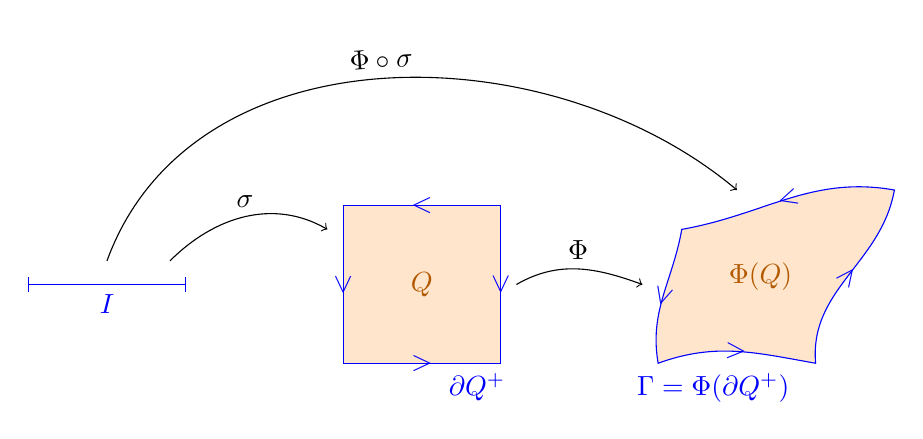
\begin{tikzpicture}
\draw[blue,|-|] (0,0) -- (2,0) node[midway,below] {$I$}; % Intervalo I

\draw[->] (1.8,0.3) to[out=45, in=150] node[midway,above] {$\sigma$} (3.8,0.7) ;

% % Primer cuadrado
\fill[orange!20!white,draw=none] (4,1) rectangle (6,-1);

\draw[blue] (4,-1) -- (4,1) node[midway,sloped] {\textless};
\draw[blue] (4,1) -- (6,1) node[midway,sloped] {\textless};
\draw[blue] (6,1) -- (6,-1) node[midway,sloped] {\textgreater};
\draw[blue] (6,-1) -- (4,-1) node[midway,sloped] {\textgreater};

\node[orange!70!black] at (5,0) {$Q$};
\node[blue,below] at (5.7,-1) {$\partial Q^+$}; 

\draw[blue, fill=orange!20!white] 
	(8,-1) to[out=100, in=260] node[midway,sloped] {\textless} 
	(8.3,0.7) to[out=10, in=170] node[midway,sloped] {\textless} 
	(11,1.2) to[out=260, in=95] node[midway,sloped] {\textgreater} 
	(10,-1) to[out=170, in=20] node[midway,sloped] {\textgreater}  (8,-1) -- cycle;

\draw[->] (6.2,0) to[out=30, in=160] node[midway,above] {$\Phi$} (7.8,0);	

\node[orange!70!black] at (9.3,0.1) {$\Phi(Q)$};
\node[blue,below] at (8.7,-1) {$\Gamma = \Phi(\partial Q^+)$};

\draw[->] (1,0.3) to[out=70, in=140] node[above,sloped] {$\Phi\circ\sigma$} (9,1.2);
\end{tikzpicture}
\caption{Esquema para la aplicación de Stokes en un cubo unidad}
\end{figure}

 Sea $\omega$ una k-forma en $\real^n$. Queremos calcular la integral de su diferencial en $Φ(Q)$.
 
\[
\int_{\Phi(Q)} \dif \omega = \int_Q \Phi^{\ast}\dif\omega = \int_Q \dif(\Phi^{\ast}\omega) = \int_{∂Q^{+}} \Phi^{\ast}\omega
\]

Donde $∂Q^{+}$ es la frontera del cubo $Q$ orientada debidamente. El último paso es aplicar el teorema anterior.

Sea $\appl{\sigma}{I}{∂Q}$. Entonces, $\appl{\Phi\circ\sigma}{I}{\Gamma}$, siendo $\Gamma$ la frontera de $\Phi(Q)$.

Aplicando esto a la integral que estamos calculando:

\[
\int_{\Phi(dQ^{+})} \omega \equiv \int{\Phi\circ\sigma(I)} = \int_I (\Phi\circ\sigma)^{\ast} \omega = \int_I \sigma^{\ast}\left(\Phi^{\ast}(\omega)\right) = \int_{\sigma(I)} \Phi^{\ast}\omega = \int_{∂Q}\Phi^{\ast}\omega
\]
Hemos llegado finalmente a que \[ \int_{∂Q^+} \Phi^{\ast} \omega = \int_{\Phi(∂Q^+)} \omega \]

Ahora querríamos dar el siguiente paso: 

\[\int_{\Phi(∂Q^+)} \omega = \int_{∂(\Phi^{\ast}(Q))} \omega \]

Es decir, que la imagen de la frontera sea la frontera de la imagen. Esto no es inmediato: en el cambio a coordenadas polares, por ejemplo, no se cumple a primera vista (ver figura \ref{imgCambioPolaresFrontera}). Cuando el ángulo (θ) se mantiene fijo y $r$ varía (segmentos azules), la imagen de esa parte de la frontera es un radio de la circunferencia, y cuando $r=0$ y variamos el ángulo (segmento verde) la imagen es un punto. 

\begin{figure}[hbtp]
\centering
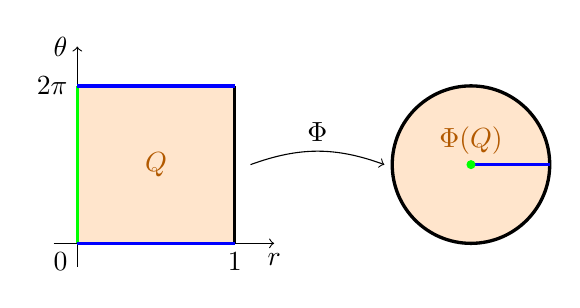
\begin{tikzpicture}
\fill[orange!20!white] (0,0) rectangle (2,2);

\draw[->] (0,-0.3) -- (0,2.5);
\node[left] at (0,2.5) {$\theta$};
\node[left] at (0,2) {$2\pi$};
\draw[->] (-0.3,0) -- (2.5,0);
\node[below] at (2.5,0) {$r$};
\node[below] at (2,0) {$1$};
\node[below left] at (0,0) {$0$};

\draw[very thick] (2,0) -- (2,2);
\draw[very thick,green] (0,0) -- (0,2);
\draw[very thick,blue] (0,2) -- (2,2);
\draw[very thick,blue] (0,0) -- (2,0);

\node[orange!70!black] at (1,1) {$Q$};

\draw[->] (2.2,1) to[out=20,in=160] node[midway,above,sloped] {$\Phi$} (3.9,1);

\draw[very thick,fill=orange!20!white] (5,1) circle (1);
\draw[very thick,blue] (5,1) -- (6,1);
\node[inner sep=1pt,circle,green,draw,fill=green] at (5,1) {};

\node[orange!70!black, above] at (5,1) {$\Phi(Q)$};

\end{tikzpicture}
\caption{La frontera no es la misma en el cambio a polares: las partes verde y azul forman parte de $∂Q$ pero no de $∂(Φ(Q))$.}
\label{imgCambioPolaresFrontera}
\end{figure}

Ahora bien, podemos dividir la región $Q$ en celdas disjuntas, como se puede ver en la figura \ref{imgPolaresDisjuntas}. De esta forma, las fronteras que sean comunes a varias celdas tendrán orientación incompatible y se anularán al integrar. Esto nos resuelve el problema y podemos enunciar el teorema de Stokes para celdas:


\begin{figure}[hbtp]
\centering
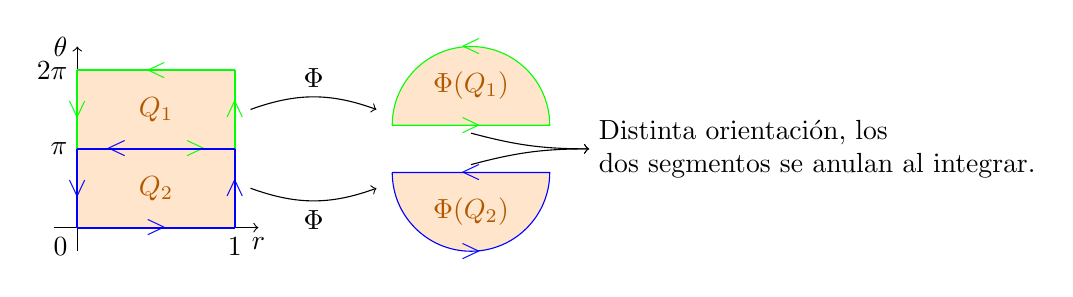
\begin{tikzpicture}
\fill[orange!20!white] (0,0) rectangle (2,2);

\draw[->] (0,-0.3) -- (0,2.3);
\node[left] at (0,2.3) {$\theta$};
\node[left] at (0,2) {$2\pi$};
\node[left] at (0,1) {$\pi$};
\draw[->] (-0.3,0) -- (2.3,0);
\node[below] at (2.3,0) {$r$};
\node[below] at (2,0) {$1$};
\node[below left] at (0,0) {$0$};

\draw[thick,green] (0,1) -- (0,2) node [midway,sloped] {\textless};
\draw[thick,green] (0,2) -- (2,2) node [midway,sloped] {\textless};
\draw[thick,green] (2,2) -- (2,1) node [midway,sloped] {\textless};
\draw[thick,green] (2,1) -- (0,1) node [near start,sloped] {\textgreater};

\draw[thick,blue] (0,0) -- (0,1) node [midway,sloped] {\textless};
\draw[thick,blue] (0,1) -- (2,1) node [near start,sloped] {\textless};
\draw[thick,blue] (2,1) -- (2,0) node [midway,sloped] {\textless};
\draw[thick,blue] (2,0) -- (0,0) node [midway,sloped] {\textgreater};

\node[orange!70!black] at (1,1.5) {$Q_1$};
\node[orange!70!black] at (1,0.5) {$Q_2$};

\draw[->] (2.2,1.5) to[out=20,in=160] node[midway,above,sloped] {$\Phi$} (3.8,1.5);
\draw[->] (2.2,0.5) to[out=-20,in=200] node[midway,below,sloped] {$\Phi$} (3.8,0.5);

\draw[green,fill=orange!20!white] (4,1.3) arc (180:0:1) -- (4,1.3) node[midway] {\textgreater};
\node[green] at (5,2.3) {\textless};
\node[orange!70!black] at (5,1.8) {$\Phi(Q_1)$};


\draw[blue,fill=orange!20!white] (4,0.7) arc (-180:0:1) -- (4,0.7) node[midway] {\textless};
\node[blue] at (5,-0.3) {\textgreater};
\node[orange!70!black] at (5,0.2) {$\Phi(Q_2)$};

\draw[->] (5,1.2) to[out=345, in=180] (6.5,1);
\draw[->] (5,0.8) to[out=15, in=180] (6.5,1);

\node[right,align=left] at (6.5,1) {Distinta orientaci\'{o}n, los\\ dos segmentos se anulan al integrar.};

\end{tikzpicture}
\caption{Podemos dividir $Q$ en dos celdas disjuntas}
\label{imgPolaresDisjuntas}
\end{figure}


\begin{theorem}[Teorema\IS de Stokes (para celdas)]\label{thmStokesCeldas}
\[ \int_M \dif \omega = \int_{\partial  M^+}\omega \]

, si la variedad $M$ se puede descomponer como unión de celdas con interior disjunto. 
\end{theorem} 

\paragraph{Frontera de una superficie}
Vamos a intentar definir en serio la frontera de objetos en $\real^3$, que es algo que necesitamos tener realmente muy claro.

\easyimg{imgs/StokesCeldasTipo.png}{ψ nos lleva $P$ a un punto que no está en la frontera de la imagen por ψ de su celda correspondiente (llamada de tipo I). En el caso de $Q$, ψ lo lleva a un punto en la frontera de la imagen de su celda por ψ (de tipo II), por lo tanto sí es un punto de la frontera.}{imgTiposCelda}

Hace un tiempo, cuando definíamos una subvariedad, demostramos la existencia de un difeomorfismo Ψ que "aplanaba un trozo" de subvariedad. La frontera de una superficie es el conjunto de los puntos (llamados en clase de Tipo 2) que al aplanar nos quedan en la frontera de un objeto de dimensión 2 (ver imagen \ref{imgTiposCelda}).
\index{Frontera}
Una vez aclarado el concepto de frontera, pasamos a demostrar el teorema de Stokes.


\begin{theorem}[Teorema\IS de Stokes]
Sea $M$ una subvariedad compacta, orientable, con frontera relativa $\partial  M$.

Entonces

\[\int_{\partial  M^+}\omega = \int_M \dif \omega \]

\end{theorem}

\begin{proof} La demostración ya está vista para celdas en la sección anterior, así que vamos a extender la idea.



\subparagraph{Paso 1: Compacidad}
Para todo punto $P\in M$ existe una celda $C_p$ tal que $P \in C_p$. Por lo tanto, está claro que $M\subset \bigcup_{p\in M} C_p$. Tomamos el interior de las celdas, para trabajar con conjuntos abiertos.

Hemos recubierto con infinitos abiertos la subvariedad, así que por compacidad (\ref{thmCerradoAcotado}) existe un subrecubrimiento \textbf{finito}.

Sin embargo, no podemos garantizar que las celdas son disjuntas. Si lo fueran, aplicaríamos el teorema a cada celda y listo. Hay que ver qué ocurre cuando las celdas no son disjuntas.

\subparagraph{Paso 2: Particiones de la unidad}

Vamos a intentar resolver el problema de los solapamientos. Buscamos una función que valga cero fuera de la celda que consideramos y sea mayor que cero dentro de ella, algo como pueda ser la figura \ref{imgStokesPhi}.

\begin{wrapfigure}{r}{0.6\textwidth}
  \begin{center}
    \includegraphics[width=0.58\textwidth]{imgs/TeoremaStokes-PartUnidad.png}
  \end{center}
  \caption{La función Φ que buscamos sería algo así.}
  \label{imgStokesPhi}
\end{wrapfigure}
Sea $\appl{\Phi}{\real^N}{\real}$. Además, 
\begin{itemize}
\item $\Phi>0$ en $\mathcal{Q}$
\item $\Phi = 0$ en $\partial  \mathcal{Q}$
\item $\Phi = 0$ en $\real^N-\mathcal{Q}$
\item $\Phi\in C^1$.
\end{itemize}
Consideramos $\Phi_i = \Phi\circ\Psi_{p_i}$, siendo $\Psi_{p_i}$ el difeomorfismo que cubre la celda $p_i$, con $i=1,...,k$ y la lleva al cubo unidad ($\mathcal{Q}$).

Además, nos gustaría que la suma de todas las aplicaciones $Φ_i$ sobre un punto sea 1:

\[ \sum_i \Phi_{i}(\gx) = 1\;\forall \gx \in M\]

Aunque parece una cosa imposible, vamos a ver que es algo perfectamente factible:

\[\tilde{\Phi}(\gx) = \frac{\Phi_i (\gx)}{\sum_{i=1}{k}\Phi_i(\gx)}\]

Estas $\tilde{\Phi}_i$ satisfacen todas las propiedades que nos interesan.

\subparagraph{Paso 3: Descomposición del problema}

Lo que nosotros queremos es calcular $\int_M d\omega$. Tal y como habíamos definido $\tilde{Φ}$ antes, es obvio que sobre la variedad $M$ 
\[ \omega=\sum_i^k\tilde{\Phi}_i(x)\omega \]

Entonces 

\[\dif \omega = \sum_{i=1}^k \dif (\tilde{\Phi}_i,\omega) = \sum_{i=1}^k \left( \dif \tilde{\Phi}_i\y \omega + \tilde{\Phi}_i \dif \omega \right) =  \dif\left(\sum_i \tilde{\Phi}_i\right) \y \omega + \sum \tilde{\Phi}_i \dif \omega\]

Dado que $\sum_i \tilde{Φ}_i = 1$, $\dif\left(\sum_i \tilde{\Phi}_i\right) = 0$ y por lo tanto

\[ \dif \omega = \sum \tilde{\Phi}_i \dif \omega \]

Aplicando esto descomponemos:
\[\int_M \dif \omega = \sum_{i=1}^k \int_M \tilde{\Phi}_i \dif\omega = \sum_{i=1}^k \int_{C_{p_i}} \tilde{\Phi}_i \dif\omega=\sum_{i=1}^k \int_{C_{p_i}} \dif(\tilde{\Phi}_i\omega)
\]

Hemos conseguido definir la integral como una suma finita de integrales sobre celdas en las que sí podemos aplicar el teorema de Stokes (\ref{thmStokesCeldas})

Entonces tenemos:

\[\int_M \dif \omega = \sum_{i=1}^k \int_{\partial  C_{P_i}^{+}} \tilde{\Phi}_i\omega\]

Por como hemos definido $\tilde{\Phi}_i$ tenemos que todas las celdas de tipo 1 valen 0. En cambio en las celdas de tipo 2 (ver \ref{imgTiposCelda} para los tipos de celda), tenemos una parte sobre la que $\tilde{\Phi}_i \neq 0$ (ver figura \ref{imgStokesCeldasIntegral}).

Esto nos deja: \[\int_M d\omega = \sum_{i=1}^k \int_{\partial  C{P_i}^{+}} \tilde{\Phi}_i\omega = \sum \int_{\partial M^+} \tilde{\Phi}_i \omega = \int_{\partial M^+} \omega\]

\end{proof}

\begin{figure}[hbtp]
  \begin{center}
    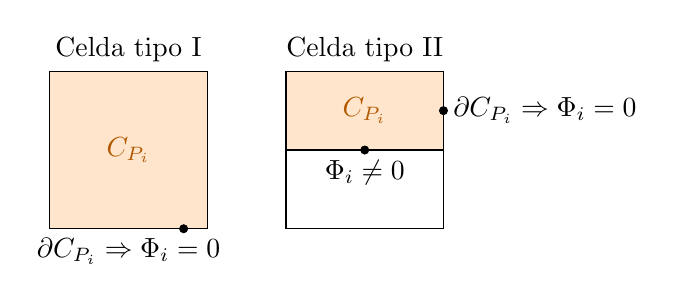
\begin{tikzpicture}
\draw[fill=orange!20!white] (0,0) rectangle (2,2);
\node[orange!70!black] at (1,1) {$C_{P_i}$};
\node[below] at (1,0) {$\partial C_{P_i} \Rightarrow \Phi_i = 0$};
\node[draw,circle,inner sep=1pt,black,fill=black] at (1.7,0) {};
\node[above] at (1,2) {Celda tipo I};

\draw[fill=white] (3,0) rectangle (5,2);
\draw[fill=orange!20!white] (3,1) rectangle (5,2);
\node[draw,circle,inner sep=1pt,black,fill=black] at (4,1) {};
\node[orange!70!black] at (4,1.5) {$C_{P_i}$};
\node[right] at (5,1.5) {$\partial C_{P_i} \Rightarrow \Phi_i = 0$};
\node[draw,circle,inner sep=1pt,black,fill=black] at (5,1.5) {};
\node[below] at (4,1) {$\Phi_i \neq 0$};
\node[above] at (4,2) {Celda tipo II};

\end{tikzpicture}
  \end{center}
  \caption{Sólo influyen a la integral los puntos de la frontera de la variedad, los que llevan a celdas de tipo II.}
  \label{imgStokesCeldasIntegral}
\end{figure}

\begin{example}
Sea $M$ una superficie en $\real^3$, un trozo de $x^2+y^2+z^2 = 1$ dentro de $x^2+y^2\leq y$, con $z\geq 0$. Ver figura \ref{imgEsferaCono}. Consideramos la orientación positiva como la de la normal hacia abajo.

\easyimg{imgs/EsferaCilindro.png}{Intersección de la esfera y el cilindro. La línea azul es la frontera de $M$, y las flechas naranjas indican su orientación positiva.}{imgs/EsferaCono}


Calcular las tres integrales

\[ \int_{\partial M} x \id y;\;\int_{\partial M} y \id z;\; \int_{\partial M} z \id x \]

\textbf{Previos} Nos damos cuenta de que $x^2+y^2\leq y$ es una circunferencia. Si completamos cuadrados tenemos la siguiente ecuación: \[x^2+\left(y-\frac{1}{2}\right)^2 = \frac{1}{4}\]

Es decir, una circunferencia de radio $\frac{1}{2}$ centrada en $(0,\frac{1}{2})$.

\paragraph{Resolución de $\int_{\partial M} x \dif y$}

\[
\int_{\partial M^{+}} x\dif y =\int_{\partial M^{+}} (0,x,0) \dif\sigma \stackrel{\mathrm{Stokes} }{=} \iint\limits_M \rot (0,x,0) \dif S = \iint\limits_M (0,0,1) \dif S
\]

Para calcular esta integral (que es calcular el flujo) aplicamos la fórmula de siempre. Para ello necesitamos parametrizar la superficie $M$:
\begin{equation}\label{eqEjStokes}
\Phi(x,y) = (x,y,\sqrt{1-x^2+y^2}), (x,y)\in D = \{x^2+y^2\leq y\} 
\end{equation}

Calculamos $T_x\x T_y =\displaystyle \left(\frac{x}{\sqrt{\cdot}},\frac{x}{\sqrt{\cdot}},1\right)$

\[
\int \int_M (0,0,1) dS = - \int \int_D \pesc{(0,0,1),(\ast,\ast,1)} \,dx\,dy = -\text{ Area } (D) = -\pi\frac{1}{4}
\]

\[ \int_{∂M^+}y\df{z} = \int_{∂M^+}(0,0,y)\df{σ} \stackrel{Stokes}{=} \int\int_{M^+} \rot (0,0,y)\df{S} \]

En \ref{eqEjStokes} teníamos la parametrización, así que la aplicamos. Teniendo en cuenta la orientación, tenemos que cambiar el signo y nos queda 

\[ 
- \iint_D \pesc{(1,0,0),\left(\frac{x}{\sqrt{\ast}}, \frac{y}{\sqrt{\ast}}, 1}\right) \df{x}\df{y} 
= -\iint_D\frac{x}{\sqrt{1-x^2-y^2}} \d{x,y} 
\]

Viendo que estamos integrando una función impar en una región simétrica, la integral vale 0.

\paragraph{Resolución de $\int_{\partial M} z \dif x$}

Pasamos ahora a calcular la integral de $z$. Tenemos lo mismo que antes:

\begin{gather*}
 \int_{∂M^+}z\df{x} = \int_{∂M^+}(z,0,0)\df{σ} \stackrel{Stokes}{=} \iint_{M^+} \rot (z,0,0)\df{S} = \iint_{M^+}(0,1,0)\id{S}= \\
 - \iint_D \pesc{(0,1,0),\left(\frac{x}{\sqrt{\ast}}, \frac{y}{\sqrt{\ast}}, 1\right)}\id{x,y} 
= -\iint_D\frac{y}{\sqrt{1-x^2-y^2}} \id{x,y}
\end{gather*}

Vemos que esta integral es muy complicada y nos va a ganar, así que pasamos a tratar de integrar como una curva. Deberemos parametrizar la curva, encontrar la orientación correcta y aplicar la fórmula.

Empezamos con la parametrización:

\[ ∂M = \left\{ \begin{matrix}
x^2+y^2+z^2 = 1 \implies y + z^2 = 1 \implies z = \sqrt{1-y} \\
x^2 + y^2 = y \implies x = \pm \sqrt{y-y^2}
\end{matrix}\right. \]

Por lo tanto, podemos parametrizar en dos trozos

\begin{align*}
Γ_1\equiv &(\sqrt{y-y^2}, y, \sqrt{1-y});\;y∈[0,1] \\
Γ_2\equiv &(-\sqrt{y-y^2}, y, \sqrt{1-y});\;y∈[0,1] \\
\end{align*}

\easyimgw{imgs/OrientacionesEsferaCilindro}{Orientaciones de $Γ_1$ y $Γ_2$}{imgs/OrientacionesEsferaCilindro}{0.7}

Tal y como vemos en la figura \ref{imgOrientacionesEsferaCilindro}, la orientación es negativa en $Γ_1$ y positiva en $Γ_2$. Entonces

\[ \int_{∂M^+}(z,0,0)\df{σ} = \int_{Γ_1^+}(z,0,0)\dif{σ_1} +  \int_{Γ_2^+}(z,0,0)\dif{σ_2} \]

Operando con la primera integral:

\[  \int_{Γ_1^+}(z,0,0)\dif{σ_1} = - \int_0^1\pesc{(\sqrt{1-y},0,0),\left(\frac{1-2y}{2\sqrt{y-y^2}},\ast,\ast\right)}\dif y = 
-\int_0^1\frac{1-2y}{2\sqrt{y}}\dif y = \]

Separamos en dos sumandos

\[ = \int_0^1\sqrt{y}\d y - \int_0^1 \frac{1}{2\sqrt y}\dif y = \dotsb \]

Podríamos tomar otra parametrización alternativa usando coordenadas esféricas. La esfera queda determinada por la parametrización

\[ \left\{\begin{matrix}
x &=& \cos θ \sin φ \\
y &=& \sin θ \sin φ \\ 
z &=& \cos φ
\end{matrix}\right. \]

Añadiendo la restricción de $x^2+y^2=y$, nos queda que $\sin φ = \sin θ$. Entonces podemos seguir parametrizando 

\[\left. \begin{matrix}
x = \cos θ \sin θ \\
y = \sin^2 θ \\
 z = \sqrt{1-\sin^2 θ} = \abs{\cos θ}
\end{matrix} \right\} θ∈[0,π]
\]

y tenemos que

\[ σ_1(θ) = (\cos θ \sin θ, \sin^2 θ, \cos θ) \]

Por otra parte, si pusiésemos los límites de integración en la región D pasaría algo.
\end{example}

\section{Campos conservativos}

\begin{defn}[Campo\IS conservativo] Consideramos $\vf$, un campo en $ℝ^N$. Se dice que $\vf$ es conservativo si y sólo si $∃\appl{V}{ℝ^N}{ℝ}$ tal que $F=\grad V$, donde $V$ es el \textbf{potencial}\index{Potencial} del campo $\vf$.
\end{defn}

\begin{theorem} Sea $\vf$ un campo $C^1$ en $ℝ^3$. Entonces $\vf $ es conservativo si y sólo si $\rot \vf = \vec{0}$.
\end{theorem} \label{consImpRot}

\begin{proof}
\paragraph{Implicación a la derecha} Como $F=\grad V$, y $F∈C^1$, entonces $V∈C^2$. Calculamos ahora el rotacional:

\[ \rot\vf = \left|\begin{matrix}
\vec{i} & \vec{j} & \vec{k} \\
\pd{}{x} & \pd{}{y} & \pd{}{z} \\
F_1 & F_2 & F_3
\end{matrix}\right| = \left(\dpa{F_3}{y}-\dpa{F_2}{z}, \dpa{F_1}{z}-\dpa{F_3}{x}, \dpa{F_2}{x}-\dpa{F_1}{y} \right) \]

Sustituyendo con $F=\grad V$ veríamos que sale todo cero.

\paragraph{Implicación hacia la izquierda}

Supongamos $Γ$ una curva cerrada, que sea la frontera de una superficie $M$. Entonces

\[ \int_{M^+}\vf  \stackrel{Stokes}{=} \iint_M\rot \vf\dif S = 0 \]

Es decir, que la integral de $F$ sobre cualquier curva cerrada va a dar 0. Buscamos ahora un $V$ tal que $\grad V = \vf$.

Supongamos un punto cualquiera $(x,y,z)$: A ese punto podemos llegar a través de varias rectas paralelas a los ejes. Con esas rectas podríamos construir un camino, y entonces tendríamos que 

\todo[inline]{Poner dibujito aquí}

\[ \int_{Γ_1}\vf = \int_{Γ_2} \vf = \int_{Γ_3}\vf \]

ya que cogiendo dos pares $Γ_i$ y cambiando la orientación de uno de ellos construimos una curva cerrada.

Parametrizamos $Γ_1$:

\[ Γ_1 \equiv \{ (t,0,0)\,t∈[0,x]\} 
	\cup \{ (x,s,0)\,s∈[0,y]\}
	\cup \{ (x,y,r)\,r∈[0,z]\} \]
	
Entonces

\begin{align*}
\int_{Γ_1}\vf&= \int_0^x\pesc{(F_1(t,0,0),F_2(t,0,0), F_3(t,0,0),(1,0,0)}\dif t \\
&+\int_0^y\pesc{(F_1(x,s,0),F_2(x,s,0), F_3(x,s,0),(0,1,0)}\dif s \\
&+\int_0^x\pesc{(F_1(x,y,r),F_2(x,y,r), F_3(x,y,r),(1,0,0)}\dif r \\
&=\int_0^x F_1(t,0,0)\dif t + \int_0^y F_2(x,s,0)\dif s+ \int_0^z F_3(x,y,r)\dif r 
\end{align*}

De la misma forma, tendríamos

\begin{gather*}
\int_{Γ_2}\vf = \int_0^y F_2(0,t,0)\dif t + \int_0^z F_3(0,y,s)\dif s+ \int_0^x F_1(x,y,r)\dif r \\ 
\int_{Γ_3}\vf = \int_0^x F_1(t,0,0)\dif t + \int_0^z F_3(x,0,s)\dif s+ \int_0^y F_1(x,r,z)\dif r \\
\end{gather*}

Las tres integrales son iguales, así que podemos derivar con respecto de la que nos venga mejor para construir la función $V$, que es la que buscábamos.

\end{proof}

La versión de este teorema vista en clase de prácticas (que es una versión más práctica)
\begin{theorem}[Campos conservativos]
$F$ es un campo vectorial $C^1$ en $\real^3$ excepto en un número finito de puntos entonces son equivalentes:
\begin{itemize}
\item Existe un potencial
\item La integral sobre una curva cerrada simple es 0
\item Las integrales por un camino o por otro para llegar a un punto son iguales
\item rot $\vf=0$.
\end{itemize}
\end{theorem}

Además, para calcular el potencial se puede utilizar cualquiera de estas 3 fórmulas:

\begin{gather*}
\int_{Γ_1}\vf=\int_0^x F_1(t,0,0)\dif t + \int_0^y F_2(x,s,0)\dif s+ \int_0^z F_3(x,y,r)\dif r \\
\int_{Γ_2}\vf = \int_0^y F_2(0,t,0)\dif t + \int_0^z F_3(0,y,s)\dif s+ \int_0^x F_1(x,y,r)\dif r \\ 
\int_{Γ_3}\vf = \int_0^x F_1(t,0,0)\dif t + \int_0^z F_3(x,0,s)\dif s+ \int_0^y F_1(x,r,z)\dif r \\
\end{gather*}

\subsection{Ejemplos}

\begin{example} Tenemos un cono de base $D$ y altura $h$, y buscamos integrar el campo $\vf(x,y,z)= (x,y,z)$. $Ω$ es el espacio del cono, y $∂Ω$, su superficie, se divide en la superficie lateral y la base.

\todo[inline]{Dibujito L1244}

Si escribimos el teorema de Gauss, tenemos que 

\[ \iiint_Ω \dv \vf \id{x,y,z} = \iint_{∂Ω^+} \vf \dif S \]

En este caso, tenemos la suerte de que $\dv \vf = 3$, y por lo tanto

\[ \iiint_Ω \dv \vf \id{x,y,z} = 3 \cdot \mathrm{Volumen}\,(Ω) \]

Por lo tanto, para hallar el volumen calculamos la integral sobre la superficie y dividimos entre tres.

La idea geométrica es que en la cara lateral, la componente normal de $\vf$ es 0. Lo vemos fácilmente sabiendo que la recta definida por el vector $(x,y,z)$ y que pasa por el origen (el vértice del cono), tiene exactamente la misma dirección de la generatriz. Entones,\textbf{ la integral sobre la cara lateral es 0} y por lo tanto podemos ignorarla. Nos centramos sólo en la integral de la base:

\[ \iint_{\mathrm{Base}}\vf \id S \]

Parametrizar $S$ es sencillo:

\[ S \equiv \{ (x,y,h)\tq (x,y)∈ D \} \]

Calculamos su vector normal:

\[ \left.\begin{matrix}
T_x = (1,0,0) \\
T_y = (0,1,0)
\end{matrix}\right\} T_x × T_y = (0,0,1) \]

y entonces

\[ \iint_{\mathrm{Base}}\vf \id S = \iint_D\pesc{(x,y,h),(0,0,1)} \id{x,y} = \iint_D h \id{x,y} = h \cdot \mathrm{Area}\,(D) \] 

Finalmente 

\[ \mathrm{Volumen}\,(Ω) = \frac{h \cdot \mathrm{Area}\,(D)}{3} \]
\end{example}

\begin{example}[Cálculo del campo eléctrico o gravitatorio]

La expresión del campo eléctrico es 

\[ \vf(\vx) = C \frac{\vx}{\norm{\vx}^3} \]

Calculando las derivadas parciales

\begin{align*}
\dpa{F_1}{x}&=\frac{y^2+z^2-2x^2}{(x^2+y^2+z^2)^{\frac{5}{2}}} \\
\dpa{F_2}{y}&=\frac{x^2+z^2-2y^2}{(x^2+y^2+z^2)^{\frac{5}{2}}} \\
\dpa{F_3}{z}&=\frac{x^2+y^2-2z^2}{(x^2+y^2+z^2)^{\frac{5}{2}}}
\end{align*}

nos queda que

\[ \dv\vf = 0 \]

Consideramos ahora una bola de radio $R$ centrada en el origen, es decir, $B_R(0,0,0)$. Integramos sobre su superficie:

\[ \iint\limits_{∂B_R^+} \vf \id{S} = 
\iint\limits_{x^2+y^2+z^2 = R^2} \left(\frac{x}{R^3},\frac{y}{R^3},\frac{z}{R^3} \right) \id S = \frac{1}{R^3} \iint\limits_{x^2+y^2+z^2 = R^2} (x,y,z)\id S = \]

Dado que integrar el vector es integrar su componente escalar, la integral nos queda

\[ = \frac{1}{R^3} \iint\limits_{x^2+y^2+z^2 = R^2} R\id{x,y} = \frac{1}{R^2}\cdot \mathrm{Area\; esfera} = 4π \]

Ahora bien, si no supiésemos ese argumento geométrico, empezaríamos parametrizando la esfera:

\[ Φ(θ,φ) =(R\cos θ \sin φ, R\sin θ\sin φ, R\cos φ);\, θ∈[0,2π], φ∈[0,π] \]

Calculamos los vectores tangentes y el normal:

\[ \left. \begin{matrix}
T_θ = (-R\sin θ \sin φ, R\cos θ \sin φ, 0) \\
T_φ = (R\cos θ\cos φ, R\sin θ \cos φ, -R\sin φ)
\end{matrix}\right\} T_θ×T_φ = -R\sin φ (R\cos θ, \]

La normal es interior, así que pagamos con un cambio de signo:

\begin{gather*} \iint\limits_{x^2+y^2+z^2 = R^2} \left(\frac{x}{R^3},\frac{y}{R^3},\frac{z}{R^3} \right) \id S = \\
- \int_0^{2π}\int_0^π\pesc{\left(\frac{R\cos θ \sin φ}{R^3},{R\sin θ \sin φ}{R^3},{R\cos φ}{R^3}\right), (,,)} = \dotsb \mathrm{Calculos\; aqui} \end{gather*}

y al final sale lo mismo que antes pero con cuentas mucho más desagrable.

¿Por qué el teorema de Gauss no funciona? La divergencia es 0 y la superficie es cerrada. Sin embargo, $\vf$ no es $C^1$ en el origen (no existe en ese punto) así que no podemos aplicarlo.

Pero, por otra parte, siempre hemos visto que la integral no se ve afectada por lo que ocurra en un punto. ¿Por qué no funciona el teorema de Gauss sólo por lo que pasa en el origen?

En realidad en el origen la divergencia vale $4π$ por un churrumillo muy raro (delta de algo) \todo{Dibujar el churrumillo}

Pero también podemos hacer un apaño. Consideramos un conjunto $Ω$, y una bola $B_ε(0,0,0)$. Entonces

\[ Ω_ε = Ω - B_ε \]

de tal forma que $\vf∈C^1$ en $Ω_ε$. Aplicando el teorema de Gauss:

\[ 0 = \iiint\limits_{Ω_ε}\dv \vf \id{x,y,z} = \iint\limits_{∂Ω_ε^+}\vf \id{S} \]

La frontera se divide en dos partes: $∂Ω_ε = ∂Ω + ∂B_ε^+$. Entonces

\[ 0 = \iint\limits_{∂Ω^+}\vf \id S - \iint\limits_{∂B_ε^+}\vf \id S \]

y por lo tanto, tenemos que 

\[ \iint\limits_{∂Ω^+}\vf \id{S} = 4π\; ∀Ω \tq 0 ∈ Ω \]

\end{example}


\begin{theorem}
Si $\vf \in C^1$

div$\vf = 0\dimplies \exists \vg\in C^2 \tlq \rot \vg = \vf$
\end{theorem}

\begin{proof}

Con el lenguaje de las formas diferenciales es muy facil esta demostración.

\todo[inline]{reescribir bien}
$vf$ es una 1-forma a la que aplicamos la diferencial exterior y obtenemos una 2-forma, que es su rotacional. Entonces, al volver a hacer la diferencial (para hallar la divergencia) es diferencial de diferencial =0.


Sin formas diferenciales tenemos:

\[G=(G_1,G_2,G_3)\]
\[\rot G = \left(\ast_1,\ast_2,\ast_3\right)\]

\[\div(\rot G) = \dpa{}{x}(\ast_1) + \dpa{}{y}(\ast_2) + \dpa{}{z}(\ast_3)\]
Por la igualdad de las derivadas cruzadas (toerema de Euler) al ser $G\in C^2$ se cancela todo.

$\implies$ Buscamos $\vg$ tal que $(F_1,F_2,F_3) = \rot \vg$.

Podemos definir el sistema:

\[\begin{array}{cc}
\dpa{G_3}{y} - \dpa{G_2}{z} &= F_1\\
\dpa{G_1}{z} - \dpa{G_3}{x} &= F_2\\
\dpa{G_2}{x} - \dpa{G_1}{y} &= F_3
\end{array}\]

Supongamos que $G_3\equiv 0$
\todo[inline]{Porque podemos suponer esto?}

\[\begin{array}{cc}
 - \dpa{G_2}{z} &= F_1\\
\dpa{G_1}{z} - &= F_2\\
\dpa{G_2}{x} - \dpa{G_1}{y} &= F_3
\end{array} \begin{array}{cc}
\longrightarrow & G_2 = -\int_0^z F_1(x,y,t)dt+A(x,y)\\
\longrightarrow & G_1 = \int_0^2 F_2(x,y,t)dt + B(x,y)\\
\longrightarrow & F_3 = \dpa{}{x} \left\{-\int_0^z F_1(x,y,t)dt + A(x,y)\right\}
- \dpa{}{y}\left\{\int_0^2 F_2(x,y,t)dt + B(x,y) \right\}
\end{array}
\]

Vamos a ver que ocurre con  $F_3$

\[-\dpa{}{x}\left(\int_0^z F_1(x,y,t)dt\right) + \dpa{A}{x} - \dpa{}{y}\int_0^z F_2(x,y,t)dt - \dpa{B}{y}\]

Por la regularidad de $F_1$ podemos meter dentro la derivada (el argumento que está detrás de esto se ve en teoría de la medida, asíque de momento nos fiamos)

\[-\left(\int_0^z \dpa{}{x}F_1(x,y,t)dt\right) + \dpa{A}{x} - \int_0^z \dpa{}{y}F_2(x,y,t)dt - \dpa{B}{y}\]
\[-\int_0^z \left(\dpa{F_1}{x} + \dpa{F_2}{y}\right)(x,y,t)dt + \dpa{A}{x} - \dpa{B}{y} \]

Utilizamos que la $\dv = 0$ que nos dice:

\[\dpa{F_1}{x} + \dpa{F_2}{y} + \dpa{F_3}{z} = 0\]

\[ = \int_0^z \dpa{F_3}{z} (x,y,t)dt + \dpa{A}{x} - \dpa{B}{y} = F_3(x,y,z) - F(x,y,z) + \dpa{A}{x} - \dpa{B}{y}\]

Hemos llegado a \[F_3(x,y,z) =  F_3(x,y,z) - F(x,y,z) + \dpa{A}{x} - \dpa{B}{y}\]
Quedando entonces definidas $A$ y $B$ así:

\[\dpa{A}{x} - \dpa{B}{y} = F_3(x,y,0)\]
Y aquí nuevamente tenemos muchas opciones. Elegimos/suponemos/tomamos $B=0$ 
\todo[inline]{porque?}

\[A(x,y) = \int_0^x F_3(s,y,0)ds + C(y)\]
\end{proof}

\subsubsection{Anexo interesante}
Vamos a ver ahora un ejemplo de cuándo se pueden meter las derivadas dentro de una integral.

\begin{example}
Tenemos un sólido a una cierta temperatura, rodeado de un amniente a otra temperatura distitnta de tal manera que el sólido va perdiendo temperatura. Queremos saber a qué temperatura estará el sólido pasa un tiempo $T$.

Partimos de la interpretación de que la temperatura mide la \emph{cantidad de calor}. 

\textbf{Concepto previo} Una olla de 100 Litros y un vasito de chupito, ambos con agua a 100 grados, ¿qué recipiente tiene más energía? Respuesta: la olla porque es más grande.

\todo{creo que es así}
Podemos calcular el calor integrando la temperatura con el volumen


Siendo $\Omega$ el sólido, y $u(x,t)$ es la temperatura en $x$ en el instante $t$. Entonces:

\[\iiint u(x,t) dx \equiv \text{ Cantidad de calor en }\Omega\text{ en }t\]

Vamos a tomar una $B_{\epsilon}(x_0)$, vamos a estudiar:
\[\dpa{}{t} \iiint_{B_{\epsilon}(x_0)} u(x,t)dx\]
 Es la variación de temperatura a lo largo del tiempo. La temperatura varía porque el calor se transmite. ¿De qué manera se transmite? Sale fuera a través de la frontera. Se habrá ganado el calor que haya entrado y se habrá perdido el calor que haya salido. ¡Es un flujo!
 (de un campo $\vec{J}$)
  
 \[\dpa{}{t} \iiint_{B_{\epsilon}(x_0)} u(x,t)dx = -\iint_{\partial B_{\epsilon}(x_0)} \vec{J}dS\]
 (El menos aparece porque queremos que la derivada sea negativa, porque el calor sale.)
 
 
 Siguiendo la idea de Leibniz de que estamos en el mejor mundo posible ,porque el calor se transmite de las zonas calientes a las zonas frías de la manera óptima, es decir, en la dirección del $-\grad$.
 
 \todo[inline]{Revisar que pasa con $\dpa{}{t}$}
 
 \[\dpa{}{t} \iiint_{B_{\epsilon}(x_0)} u(x,t)dx = -\iint_{\partial B_{\epsilon}(x_0)} \vec{J}dS = \iint_{\partial B_{\epsilon}(x_0)}\]
 \[ = -\grad_x u dS \stackrel{Gauss}{=} \iiint_{B_{\epsilon}(x_0)} \dv(\grad_x u) = \iiint_{B_{\epsilon}(x_0)}  \]

\[ = \iiint_{B_{\epsilon}(x_0)} \dpa{u}{t}-Au\,dx=0,\forall \epsilon\]

Como lo que integramos es continua (lo llamamos $f$)

Tenemos:
\[m_{\epsilon} \leq \frac{1}{Vol(B_{\epsilon})} \iiint f \leq M_{\epsilon}\] 

Si $\epsilon \to 0$ entonces $\displaystyle\iiint_{B_{\epsilon}(x_0)} f = f(x_0)$

Entonces tenemos que \[\dpa{u}{t}(x_0,t) - Au(x_0,t) = 0\]

Y de aquí deducimos las 3 ecuaciones de transmisión de calor, que son: 
\todo[inline]{no se cuales son}
 \end{example}

Para este ejemplo ha sido fundamental el meter dentro una derivada ($\dpa{}{t}$) dentro de la integral.

Ahora vamos a ver otro ejemplo en el que esto no se puede aplicar:

\begin{example}
\todo{Dibujo}
\[\int_0^1 f_n(x)dx = \frac{1}{2}\]
\[\lim_{n\to\infty}\int_0^1 f_n(x)dx = \frac{1}{2}\]
\[\int_0^1 \lim_{n\to\infty} f_n(x) = \int_0^1 0dx = 0\]

Estamos cometiendo un error... que no vamos a contar cuál es, que se verá en teoría de la medida.
\end{example}

Nos podemos plantear en qué condiciones es cierto (en el ejemplo anterior es falso):

\[\lim_{n\to\infty} \int_{\Omega}\frac{u(x,t+1/u)-u(x,t)}{1/u} \,dx = \int_{\Omega}\lim_{n\to\infty}\frac{u(x,t+1/u)-u(x,t)}{1/u} \,dx
\]

Lo primero que tenemos que definir es la \textbf{convergencia de una sucesión a una función.} Vamos a ver un plan de interpretaciones.

\subparagraph{\textit{Convergencia puntual}}

$\forall x\in\Omega$, dado un $\epsilon>0\\ \exists n_0 \tlq n>n_0 \implies \abs{f_n(x)-f(x)}<\epsilon$

\begin{example}
1) \[f(x) = \left\{\begin{array}{cc}
1 & x\in[0,1]\cap \rac\\
0 & x\in[0,1]\cap\{\real-\rac\}
\end{array}\right.\]
Este es el ejemplo de función no integrable por Riemman (las sumas superriores valen 1 y las sumas inferiores valen 0, debido a la numerabilidad de los Racionales)

2)
Nosotros podemos definir una función de la siguiente manera: 

\[f_n(x) = \left\{\begin{array}{cc}
1 & x=r_1,...,r_n\\
0 & x\in\real-\{r_1,...,r_n\}
\end{array}\right\}\]
Siendo $r_i\in\rac$. Como es un conjunto numerable podemos definir un orden.

Continua excepto en un nº finito de puntos $\implies$ integrable de Riemman.

3) $f_n(x)\to f(x) \forall x\in[0,1]$


\textbf{Conclusión} En este caso tenemos que la convergencia puntual podemos no tener integral. 
\end{example}

Para solucionar este problema podemos definir otra noción de límite que nos evite este problema u otra noción de integral.

\subparagraph{\textit{Convergencia uniforme}}

Dado $\epsilon>0\,\exists\,n_0=n_0(\epsilon) \tlq n_0>n_0 \implies \abs{f_n(x) - f(x)} < \epsilon\, \forall x\in\Omega$.

Es decir, ${sup}{x\in\Omega} \abs{f_n(x)-f(x)} = \md{f_n-f}_{\infty} <\epsilon$.

La misma idea que con continuidad uniforme, para todos los $x$ del intervalo nos vale el mismo $n_0$.

Utilizando esta definición en el ejemplo de los triángulos, no podemos definir la sucesión que sea convergente uniformemente.

\begin{theorem}[Convergencia uniforme]
Sea $\Omega$ un dominio acotado en $\real^N$. 

Si $f_n \to f$ converge uniformemente en $\Omega$

\textbf{entonces}
\[\lim_{n\to\infty} \int_{\Omega} f_n(x)\,dx = \int_{\Omega} \lim_{n\to\infty} f_n(x)\,dx = \int_{\Omega} f(x)\,dx\]

Es decir, el límite y la integral son intercambiables.
\end{theorem}

\begin{proof}
\[0\leq\abs{\int_{\Omega}f_n(x) - f(x) \, dx} \leq <\int_{\Omega} \epsilon \,dx =\epsilon\abs{\Omega} \to 0\]
\end{proof}

\begin{theorem}
\[\left.\begin{array}{cc}
\{f_n\} \text{ continua }\\
f_n \to f \text{ uniforme en } \Omega \end{array}
\right\} \implies f \text{ continua}\]
\end{theorem}
\obs Si tenemos convergencia unifirme, tenemos una función continua. Parace una cosa tan tan buena que incluso se pasa de buena, porque no podemos trabajar con discontinuidades

\obs Adelantamos un teorema de teoría de la medida que dice \textit{ Casi todas las funciones son casi continuas en casi todos los puntos}


\begin{proof}
\[\abs{f(x) - f(y)} = \abs{f(x) \pm f_n(x) \pm f_n(y) - f(y)}\]

Elegimos un subíndice $n$ para el que se cumpla $\abs{f_n(t) - f(t)} < \frac{\epsilon}{3}$

Además, como $f_n$ son continuas, tenemos que haciendo tender $x\to y \implies f(x) - f(y) \leq \epsilon \implies$ continuidad
\end{proof}


\paragraph{Aplicación}

Sea $f_n(x) = \frac{u(x,t+1/u) - u(x,t_0)}{1/u}$

$f(x) = \dpa{u}{u}(x,t_0)$

Vamos a comprobar la convergencia uniforme:

\[0\leq \abs{f_n(x) - f(x)} \leq \abs{\frac{u(x,t+1/u) - u(x,t_0)}{1/u} - \dpa{u}{u}(x,t_0)} \stackrel{TVM}{=} \abs{\dpa{u}{t}(x,s) - \dpa{u}{t}(x,t_0)} < \epsilon \forall x\]
Donde $s\in [t_0,t_0+\frac{1}{n}]$

En el último paso utilizamos la continudad de la derivada y la compacidad (que nos da continuidad uniforme)


\subparagraph{Integral de Lebesgue}
La otra opción para poder intercambiar límites con integrales podíamos ser más estrictos con la convergencia, o mejorar la integral (aparte de todo un mundo de posibilidades intermedias del \textit{Análisis funcional}) 

Algo de esto ya vimos al hablar de integrales: (\ref{IntLebesgue})

Esto nos genera el problema de la medida de un intervalo. 
Es razonable pedir:
\begin{itemize}
\item $\abs{(a,b)} = \abs{b-a}$
\item La medida del intervalo tiene que ser invariante si le aplicamos traslaciones
\item $A\cap B = Ø $

$\abs{A \cup B} = \abs{A} + \abs{B}$
\item $A_i \cap A_j = Ø, i\neq j$

$\abs{\bigcup_{i=1}^{\infty} A_i} = \sum_{i=1}^{\infty} \abs{A_i}$.


\end{itemize}
El último requisito es un verdadero dolor de cabeza, trabajar con sumas infinitas y con uniones infinitas. Sería fácil (con la medida exterior) para conseguir un $\leq$ que no es suficiente.

Para solucionar todo estos problemas hay que definir una nueva teoría con la que casi todo es medible (salvo unos cuantos monstruos, que para encontrarlos hay que hablar del Axioma de elección)

Toda esta teoría de la integral de Lebesgue nos da resultados mucho más generales para poder intercambiar el límite con la integral, con la convergencia monótona y la convergencia domiante.

\newpage
\appendix
% -*- root: ../TIM.tex -*-
\section{Hoja 1}
\begin{problem}[1]
Demuestra que el valor absoluto de una función integrable Riemann es también integrable Riemann

\solution

Vamos a definir:
$f^+(x) = \max\lbrace f(x), 0 \rbrace$

$f(x) = f^+(x) - f^-(x)$

De donde podemos deducir:

$f^-(x) = f^+(x)-f(x)=\max \lbrace -f(x), 0 \rbrace$

Y las funciones tienen el siguiente aspecto:

\begin{center}
	% Función f
	\inputtikz{img1-ej1-h1}
	% Función f+
	\inputtikz{img2-ej1-h1}
	% Funcion f-
	\inputtikz{img3-ej1-h1}
\end{center}


Así podemos escribir \[ \abs{f(x)} = f^+(x)+f^-(x) \]

Gracias a esta afirmación el problema se reduce a demostrar que la parte positiva ($f^+$) es integrable Riemann, ya que entonces lo serán  y $f^-$  y $\abs{f(x)}$  por ser la suma/resta de dos funciones integrables Riemann.


Vamos a calcular $f^+(x)$:
\[\overline{J}_P(f^+)-\underline{J}_P(f^+) = \sum_{k=1}^n\left(\sup_{x\in I_k}(f^+(x))\right)\abs{I_k} - \sum_{k=1}^n\left(\inf_{x\in I_k}(f^+(x))\right)\abs{I_k}=\]
\[= \sum_{k=1}^n\left(\sup_{x\in I_k}(f^+(x))-\inf_{x\in I_k}(f^+(x))\right)\abs{I_k} \leq
\sum_{k=1}^n\left(\sup_{x\in I_k}(f(x))-\inf_{x\in I_k}(f(x))\right)\abs{I_k} =\] \[=\overline{J}_P(f)-\underline{J}_P(f) = 0\]

Puesto que $f$ es integrable
\end{problem}

\begin{problem}[2]
Sean $f,g$ funciones integrables Riemann en el intervalo [a,b]. Demuestra que $h(x)=\max\{f(x),g(x)\}$ es integrable Riemann. Este resultado se extiende con facilidad al máximo de un número finito de funciones. Muestra que en general no es cierto para una sucesión

\textbf{Indicación:}
\[\sup_{I_k}\{\max\{f(x),g(x)\}\}-\inf_{I_k}\{\max\{f(x),g(x)\}\} \geq \]
\[\geq \max\{\sup_{I_k}f(x)-\inf_{I_k}f(x), \sup_{I_k}g(x)-\inf_{I_k}g(x)\}\]

\solution
Vamos a comprobar que la diferencia entre las integrales Riemann superior e inferior es 0.
Pero antes fijémonos en la \underline{indicación}:

\[\sup\big\{ \max\{f(x), g(x)\}\big\} - \inf\big\{ \max\{f(x), g(x)\} \big\} \leq \]

\[ \leq \max\big\{ \sup_{x \in I_k} (f(x)) - \inf_{x \in I_k} (f(x)), \sup_{x \in I_k} (g(x)) - \inf_{x \in I_k} (g(x)) \big\} \leq \]

\[ \leq \left(\sup_{x \in I_k} (f(x)) - \inf_{x \in I_k} (f(x))\right) + \left(\sup_{x \in I_k} (g(x)) - \inf_{x \in I_k} (g(x))\right) \]


Ahora podemos probar que:
\[\overline{J}_P(h)-\underline{J}_P(h)
= \sum\left(\sup_{x\in I_k}(h(x))-\inf_{x\in I_k}(h(x))\right)\abs{I_k} \leq\]


\[\leq \sum\left( \sup_{x \in I_k} (f(x)) - \inf_{x \in I_k} (f(x)) \right) \abs{I_k} +
 \sum\left( \sup_{x \in I_k} (g(x)) - \inf_{x \in I_k} (g(x)) \right) \abs{I_k} \]

Sabiendo que $f$ y $g$ son integrables Riemann llegamos a:
\[\sum\left( \sup_{x \in I_k} (f(x)) - \inf_{x \in I_k} (f(x)) \right) \abs{I_k} +
 \sum\left( \sup_{x \in I_k} (g(x)) - \inf_{x \in I_k} (g(x)) \right) \abs{I_k} \leq 0 + 0 = 0\]

 Con lo que queda probado que $h(x) = \max\lbrace f(x), g(x) \rbrace$ es integrable Riemann

\end{problem}

\begin{problem}[3]
Sea $\{q_1,q_2,q_3,...\} = I \cap \rac$ una enumeración de los racionales de un intervalo $I=[a,b]$. Para cada $k=1,2,3,...,$ sea
\[Y_k(x)= \left\{ \begin{array}{lcc}
             1 &   si  & x \in \{q_1,q_2,q_3,...\} \\
             \\ 0 &  si  & x \notin I \setminus \{q_1,q_2,q_3,...\}
             \end{array}
   \right.\]

Demuestra que $Y_k$ es integrable Riemann.

Sea $Y(x)=\lim_kY_k(x)$, demuestra que $Y$ no es integrable Riemann.

\solution

Ya hemos visto en teoría la demostración de que toda $Y_k$ es integrable Riemann. La idea se basa en descomponerla en una suma de funciones, cada una de las cuales vale 1 en un racional y 0 en el resto.

Tomando intervalos suficientemente pequeños podemos probar que estas funciones son integrables Riemann con integral, por lo que $Y_k$ será integrable por ser suma de funciones integrables.

Para el caso $Y(x)=\lim_kY_k(x)$, vamos a ver que no es integrable Riemann viendo que las sumas superior e inferior no coinciden.

Para cualquier intervalo que cojamos, siempre vamos a tener algún racional, de modo que $\sup_{x \in I_k} (f(x)) = 1 \ \forall I_k$, pero también tendremos siempre un irracional por lo que $\inf_{x \in I_k} (f(x)) = 0 \ \forall I_k$.

Así, vemos sencillamente que la suma superior nos dará la longitud del intervalo mientras que la inferior nos dará 0
\end{problem}

\begin{problem}[4]
Con la notación del ejercicio anterior, sea
\[Z(x)= \left\{ \begin{array}{lcc}
             \frac{1}{k} &   si  & x = q_k \\
             \\ 0 &  si  & x \notin I \setminus \rac
             \end{array}
   \right.\]

Demuestra que la función $Z$ así definida es integrable Riemann en $I$ y calcula $\in_a^bZ(x)dx$

\solution

Vamos a construir la sucesión de funciones $Z_n$ similar a las del apartado anterior
\[Z_n(x)= \left\{ \begin{array}{lcc}
             \frac{1}{k} &   si  & x \in \{q_1,q_2,q_3,...,q_n\} \\
             \\ 0 &  si  & x \notin I \setminus \{q_1,q_2,q_3,...,q_n\}
             \end{array}
   \right.\]

Vemos que esta sucesión converge uniformemente a $Z(x)$ puesto que
\[\forall \epsilon, x \exists N  \tq \forall n > N, \ |Z_n(x)-Z(x)|<\epsilon\]
Si nos fijamos, vemos que $|Z_n(x)-Z(x)|<\frac{1}{n+1}$, de modo que si forzamos que $\frac{1}{n+1}<\epsilon$ estará probada la convergencia uniforme.

Basta con tomar $N=\frac{1}{\epsilon} -1$.

Una vez probada la convergencia uniforme, sabemos que $Z(x)$ es integrable y que
\[\int_a^b \lim Z_n(x) =\lim \int_a^b Z_n(x) = \lim 0 = 0\]
Sabemos que $\int_a^b Z_n(x)$ puesto que es un caso equivalente al del ejercicio anterior.
\end{problem}

\begin{problem}[5]
Dada una sucesión $\lbrace f_n \rbrace \in R([a,b])$ que converge uniformemente a $f$, se pide demostrar que $f$ es integrable Riemann y que:
\[ \lim \int_{a}^{b} f_n = \int_{a}^{b} f \]

\solution
Supongamos que f es integrable Riemann, entonces tenemos que ver que:
\[ \forall \epsilon > 0 \ , \exists N \tq \forall n> N \ \abs{\int_a^b f_n - \int_a^b f} < \epsilon\]

Sabemos que:
\[\abs{\int_a^b f_n - \int_a^b f} \leq \abs{\int_a^b \abs{f_n -f}} dx\]

Recordemos la definición de convergencia uniforme

\begin{defn}[Convergencia\IS uniforme]
\[f_n \xrightarrow{uniforme} f \Leftrightarrow \forall \epsilon < 0, \exists N_{\epsilon} \tq \forall x \in [a,b]  \forall n \geq N_{\epsilon}, \abs{f_n (x) - f(x)} < \epsilon\]
\end{defn}

Si $n \geq N_{\frac{\epsilon}{b-a}}$ entonces, usando la definición de convergencia uniforme:

\[\int_a^b \abs{f_n(x) - f(x) dx} \leq \int_a^b \frac{\epsilon}{b-a}dx = \epsilon\]

Por tanto queda claro que si $f$ es integrable Riemann podemos conmutar el límite con la integral. Ahora queda ver por qué $f$ es integrable Riemann.

$f$ será integrable Riemann sii:
\[\forall \epsilon > 0 \ \exists P \tq \forall P' \prec P \]
\[\overline{J}_{P'}(f) - \underline{J}_{P'}(f) < \epsilon\]

Vamos a probarlo:
\[\overline{J}_P(f) - \underline{J}_P(f) = \sum(\sup_k f - \underset{k}{inf} f)\abs{I_k} \leq\]
\[\leq \sum\left( \abs{\sup_{k}f(x) - \sup_{k}f_n(x)} + \abs{\sup_{k}f_n(x) - \underset{k}{inf}f_n(x)} +  \abs{\underset{k}{inf}f_n(x) - \underset{k}{inf}f(x)} \right)\abs{I_k} \leq \]
Puesto que $f_n$ converge uniformemente a $f$ habrá un $n$ a partir del cual la distancia máxima entre $f_n$ y $f$ sea $\frac{\epsilon}{6}$ y por tanto la distancia máxima entre el supremo y el ínfimo de $f_n$ será menor que $\frac{\epsilon}{3}$
\[\leq \sum\left( \sup_{k} \abs{f_n(x) - f(x)} + \frac{\epsilon}{3} + \sup_k \abs{f_n(x) - f(x)} \right)\abs{I_k} \leq\]
Aplicando de nuevo la convergencia uniforme y tomando el máximo entre este $n$ y el calculado en el paso interior nos queda:
\[\leq \sum \left(\frac{\epsilon}{3} + \frac{\epsilon}{3} + \frac{\epsilon}{3} \right)\abs{I_k} = \sum\epsilon\abs{I_k}\]

Como hay convergencia uniforme entre $f_n$ y $f$ podemos hacer que los supremos sean tan pequeños como queramos y hacer así que el interior sumatorio quede menor que $\epsilon \abs{I_k}$

Puesto que $\epsilon$ es un número cualquiera podemos hacerlo tan pequeño como queramos haciendo que el último sumatorio escrito tienda a 0.

\end{problem}

\begin{problem}[6]

Sea $\lbrace f_n \rbrace$ una sucesión monótona creciente de funciones continuas en un intervalo $I=[a,b]$ que convergen en dicho intervalo a otra función continua $f$. Demuestra que entonces:
\[ lim \int_{a}^{b} f_n(x) = \int_{a}^{b} f(x) \]
\solution
Por ser funciones continuas son integrables Riemann. Si conseguimos demostrar que convergen uniformemente podemos emplear el ejercicio anterior y lo tendríamos hecho.

Vamos a ello.

%TODO solución del libro: "Fundamentos de análisis moderno, volumen 1"

Lo que queremos demostrar coincide exactamente con el \textbf{Teorema de Dini}.
Procedamos a demostrarlo.

Para cada $\epsilon > 0$ y cada $x\in[a,b]$ existe un índice $n(x)$ tal que:
\[\forall m\geq n(x), \ f(x)-f_m(x) \leq \frac{\epsilon}{3}\]
Por ser $f$ y $f_{n(x)}$ continuas, existe un intervalo abierto $x\in(a_x,b_x)$, tal que:
\[\forall y \in (a_x,b_x), \ |f(x)-f(y)| \leq \frac{\epsilon}{3} \text{ y } |f_{n(x)}(x)-f_{n(x)}(y)| \leq \frac{\epsilon}{3}\]

Por tanto, para cada $y\in(a_x, b_x)$ se tiene:
\[|f(y)-f_{n(x)}(y)| = |f(y)-f(x)+f(x)-f_{n(x)}(x)+f_{n(x)}(x)-f_{n(x)}(y)|\leq \epsilon\]
Tómese ahora un número finito de puntos $x \in [a,b]$ tales que $(a_x,b_x)$ recubran $I$ y sea $n_0$ el mayor de los enteros $n(x)$. Entonces para cada $y\in I$, $y$ pertenece a uno de estos $(a_x,b_x)$, por tanto:

\[ \forall n\geq n_0, f(y)-f_n(y) \leq \epsilon\]

\end{problem}

\begin{problem}[7]
Dada la sucesión $I_k = (a_k, b_k)$ tales que $\bigcup_{k=1}^{N}~I_k~=~[a,b]$

Demostrar que:
\[b-a \leq \sum_{k=1}^N (b_k - a_k)\]

\solution
Vamos a utilizar la integral de Riemann como recomienda el ejercicio, utilizando la función indicatriz de cada intervalo $\ind_{I_k}$

Está claro que la función indicatriz del intervalo I es menor o igual que la suma de las funciones indicatrices de los intervalos. Lo cual es obvio, ya que si $x$ está en el intervalo, $x$ estará también en al menos uno de los intervalos $I_k$. Es decir:
\[\ind_{[a,b]} \leq \sum_{k=1}^{N} \ind_{I_k}\]

Utilizando la monotoneidad de la integral de Riemann podemos ``integrar a ambos lados'' obteniendo:

\[\int_{a}^{b} \ind_{[a,b]} \leq \int_{a_k}^{b_k} \sum_{k=1}^{N} \ind_{I_k}\]

Por la linealidad de la integral, podemos incluso meter la integral dentro del sumatorio
\[\int_{a}^{b} \ind_{[a,b]} \leq \sum_{k=1}^{N} \int_{a_k}^{b_k} \ind_{I_k}\]


Conociendo la integral de la función indicatriz tenemos el resultado de forma inmediata.
\[b-a \leq \sum_{k=1}^{N} ( b_k - a_k )\]

\end{problem}

\begin{problem}[8]
Demuestra que para cualquier conjunto $C\subset [a,b]$
\[cont^+(C) = \inf \{\sum_{n=1}^N\abs{I_n} \tq C \subset I_1 \cup I_2 \cup ... \cup I_N \text{ siendo } I_n=[a_n,b_n]\}\]

\solution

Recordemos que
\[cont^+(C)=\overline{J_P}\ind_C(x) = \sum_{n=1}^{\infty}\sup\{\ind_C(x)\}|I_k|\]
pero el supremo de la función indicatriz en un intervalo es 1 (en ese intervalo la función indicatriz siempre valdrá 1.)

Por tanto
\[cont^+(C)=\overline{J_P}\ind_C(x) =  \sum_{n=1}^{\infty}|I_k| \geq \inf \{\sum_{n=1}^N\abs{I_n} \tq C \subset I_1 \cup I_2 \cup ... \cup I_N \text{ siendo } I_n=[a_n,b_n]\}\]
por cumplir los $I_k$ la condición dada y tener a la izquierda un ínfimo.

Si logramos probar ahora la desigualdad contraria tendremos el ejercicio resuelto.
Para ello, podemos fijarnos en que
\[\forall N \  \sum_{n=1}^{\infty}|I_k| \geq \sum_{n=1}^{\infty}|I'_k| \]
ya que en el lado de la derecha, los $I'_k$ son disjuntos y su unión es exactamente $C$.

Por tanto, queda claro que la fórmula dada para el contenido de $cont^+(C)$ es válida

\end{problem}

\begin{problem}[9]
Dado $O\subset (a,b)$ unión numerable de intervalos disjuntos, se pide demostrar:
\[m^*(O)=\sum_{n=1}^{\infty} \abs{I_k}\]

\solution
Por definición de medida exterior, está claro que:
\[m^*(O)=\inf\{\sum_{k=1}^{\infty}|I_k| \tq O \subset \bigcup_{k=1}^{\infty}\} \leq \sum_{k=1}^{\infty} \abs{I_k}\]
Vamos a probar ahora que $m^*(O) \geq \sum_{k=1}^{\infty} \abs{I_k}$ y tendremos la igualdad buscada.\\
Puesto que sabemos que la suma infinita tiene resultado finito (no puede superar la longitud del intervalo $(a,b)$ ya que todos los $I_k$ se contienen en él y son disjuntos), sabemos que:
\[\forall \epsilon > 0 \exists N \tq \sum_{k=1}^{N} \abs{I_k} \geq \sum_{k=1}^{\infty} \abs{I_k} - \frac{\epsilon}{2}\]
Definimos ahora unos intervalos $I'_k$ más pequeños de la forma:
\[I'_k=[a_k+\frac{\frac{\epsilon}{2}}{2^{k+1}}, b-\frac{\frac{\epsilon}{2}}{2^{k+1}}]\]
Así:
\[\sum_{k=1}^{N}|I'_k| = \sum_{k=1}^{N}|I_k|-\frac{\epsilon}{2}\sum_{k=1}^{N}\frac{1}{2^k} \geq \sum_{k=1}^{N}|I_k|-\frac{\epsilon}{2}\]
Definimos ahora el compacto formado por la unión de estos $I_k$ compactos:
\[K =\bigcup_{k=1}^{N}I'_k \subset O\]
Sean $J_k$ intervalos abiertos que recubren $O$, también recubren $K$. Por ser $K$ compacto, dado un recubrimiento podemos encontrar un recubrimiento finito, es decir:
\[\exists N' \tq K \subset \bigcup_{k=1}^{N'}J_k = A_N\].
Volviendo a la medida exterior de O, tenemos que:
\[m^*(O) = \inf \{\sum_{k=1}^{\infty}|J_k|\} \geq \inf\{\sum_{k=1}^{N'}|J_k|\} \geq \inf\{\sum_{k=1}^{N'}|I'_k|\} \geq \inf\{\sum_{k=1}^{N'}|I_k|-\frac{\epsilon}{2}\} \geq \inf \{\sum_{k=1}^{\infty} \abs{I_k} -\epsilon\} \forall \epsilon\]
Por ser cierta la desigualdad para todo $\epsilon$ se deduce que:
\[m^*(O) \geq \inf \{\sum_{k=1}^{\infty}|I_k|\}\]
\end{problem}

\begin{problem}[10]
Dado un compacto K contenido en el intervalo (a,b), nos piden demostrar que:
\[m(K)<b-a\]

\solution
Consideremos la sucesión: $(a+\frac{1}{n}, b - \frac{1}{n})$, con $n >\frac{2}{b-a}$. Obviamente:
\[K \subset \bigcup_{n=n_0}^{\infty}(a+\frac{1}{n}, b - \frac{1}{n})\]

Como K es compacto:
\[\exists N \tq K \subset \bigcup_{n=n_0}^{N}(a+\frac{1}{n}, b - \frac{1}{n}) = (a+\frac{1}{N}, b - \frac{1}{N}) \]

Y llegamos a:
\[m(K) \leq b-a-\frac{2}{N} < b-a\]

\end{problem}

\begin{problem}[11]
Sea $C_n$ una sucesión creciente (es decir: $C_1\subset C_2 \subset C_3...$) de subconjuntos medibles de (a,b). Sea $C=\bigcup C_n$. Demuestra que $m(C_n)$ es una sucesión creciente con límite $m(C)$
\solution
Está claro que $m(C_n)$ es una sucesión creciente puesto que, por las propiedades de la medida exterior, se cumple que:
\[C_1 \subset C_2 \Rightarrow m^*(C_1) \leq m^*(C_2)\]
y al ser conjuntos medibles, $m(C) = m^*(C)$, con lo que nos queda:
\[C_1 \subset C_2 \Rightarrow m(C_1) \leq m(C_2)\]

Sabemos además que la sucesión es acotada puesto que nunca puede superar $m((a,b))$, ya que:
\[\forall i, C_i \subset (a,b) \Rightarrow \forall i, m(C_i)\leq m((a,b))\]

La sucesión de las medidas convergerá si:
\[\lim_{n \to \infty}m(C_n) = m(C) \iff \forall \epsilon > 0 \exists n_0 \tq \forall n > n_0, m(C)-m(C_n)<\epsilon\]

Vamos a demostrar que converge por reducción al absurdo.\\
Supongamos que no converge, entonces:
\[\exists ε > 0 \tq \forall n \ m(C)-m(C_n) > \epsilon\]
En ese caso, por ser medibles tanto los $C_n$ como $C$, tendríamos que:
\[m(C\setminus C_n) > \epsilon \Rightarrow \exists x \in C \wedge x \notin C_n \Rightarrow C\neq \bigcup C_n\]
Y llegamos a contradicción.

\end{problem}

\begin{problem}[12]
Sea $C_n$ una sucesión decreciente de subconjuntos medibles contenidos en (a,b) y sea $C$ la intersección de estos subconjuntos. Se pide demostrar que:
\[m(C_n) \searrow m(C)\]
\solution

Tomando los complementarios, que también son medibles, tenemos una sucesión creciente de subconjuntos medibles contenidos en (a,b). Aplicando el ejercicio anterior llegamos a que:
\[(b-a)-m(C_n) \rightarrow (b-a)-m(C)\]
De donde puede deducirse que $m(C_n)$ decrece hacia $m(c)$.
\end{problem}


\begin{problem}[13]
Sea $C_n$ una sucesión creciente de subconjuntos medibles de $\real$. Demuestra que
\[\lim_nm(C_n) \nearrow m(\bigcup C_n)\]

Sea $C_n$ una sucesión decreciente de subconjuntos medibles de $\real$. Demuestra que si existe $n_0$ tal que $m(C_{n_0}) < \infty$ entonces
\[\lim_nm(C_n) \searrow m(\bigcap C_n)\]

Da un contraejemplo que muestre que sin la condiciones de la finitud de al menos una de las medidas el resultado puede ser falso.

\solution

\textcolor{blue}{Hecho por mi, no fiarse al 100\%}

Para la primera parte podemos repetir la prueba del ejercicio 11 considerando que $C$ es un conjunto medible. En caso de no serlo tampoco tendríamos problemas puesto que las medidas convergerían a infinito.

Para el segundo apartado, si consideramos la finitud de una de las medidas, podemos emplear $C_0$ como conjunto respecto al cual calcularemos los complementarios, replicando así la demostración del ejercicio 12.

En este caso, la finitud de al menos uno de los intervalos si es necesaria ya que de lo contrario podríamos tener conjuntos infinitos con intersección vacía, lo que causaría que el límite de las medidas se nos fuese a infinito mientras la intersección permanece vacía y, por tanto, con medida 0.

\end{problem}
\newpage
\begin{problem}[14]
Dada una sucesión $A_n$ contenida en (a,b), se pide demostrar que:
\[\lim_n m(A_0\Delta A_n)=0 \Rightarrow \lim_n m(A_n)=m(A_0) \]

Recordemos que:
\[ A_n \Delta A_0 = (A_n \setminus A_0) \cup (A_0 \setminus A_n) =
(A_n \cup A_0)\cap(A_n^c \cup A_0^c) \]

\solution

\[\lim_n m(A_0\Delta A_n)=0 \Rightarrow \lim_n m(A_0^c \cap A_n)=0 \wedge \lim_n m(A_0\cap A_n^c)=0\]

Escribimos ahora $A_n$ y $A_0$ como:
\[A_n = (A_n \cap A_0) \bigcup (A_n \cap A_0^c)\]
\[A_0 = (A_0 \cap A_n) \bigcup (A_0 \cap A_n^c)\]

De aquí podemos ver que:
\[m(A_n) = m(A_n \cap A_0) + m(A_n \cap A_n^c)\]
\[m(A_0) = m(A_0 \cap A_n) + m(A_0 \cap A_n^c)\]

Y restando llegamos a:
\[m(An) = m(A_0) -m(A_0 \cap A_n^c) + m(A_n \cap A_0^c)\]

Y sabemos que las medidas de estas intersecciones tienden a 0.
\end{problem}

\begin{problem}[15]
\textbf{Conjunto ternario de Cantor}.Construye el conjunto K de la siguiente manera: $K_0=[0,1]$, $K_1$ se obtiene a partir de $K_0$ suprimiendo el intervalo abierto central de longitud $r=\frac{1}{3}$. $K_1$ es entonces la unión de dos intervalos cerrados de longitud $\frac{1}{3}$.. $K_2$ se obtiene suprimiendo de cada uno de los dos intervalos de $K_1$ su intervalo abierto central de longitud $r^2=\frac{1}{9}$ Si se continúa el proceso see obtiene una sucesión de cerrados $K_n$
en la que cada uno de ellos es unión de $2^n$ intervalos cerrados, cada uno de longitud $3^{-n}$:
\[K_0 \supset K_1 \supset ... \searrow K=\bigcap_nK_n\]

Demuestra que $K$ es compacto en $\real$ (y por tanto medible), que no contiene intervalos abiertos, que no tiene puntos aislados, y que $m(K)=0$.

\solution

\textcolor{blue}{Hecho por mi, no fiarse al 100\%}

En cada iteración estamos extrayendo del conjunto $K_0$ una serie de intervalos abiertos y, al final, el conjunto que nos queda es la diferencia entre un cerrado y un abierto contenido en él.

Por tanto el complementario de nuestro conjunto es la unión del complementario de $K_0$ y todos los abiertos que hemos ido extrayendo, es decir, su complementario es una unión de abiertos que es abierta, por lo que tenemos que el conjunto $K$ es cerrado y acotado (sigue contenido en $K_0$).

Por ser un conjunto cerrado y acotado en $\real$ obtenemos que es compacto.

En cada paso, extraemos un intervalo de longitud $\frac{1}{3}$ y evitamos la existencia de intervalos abiertos de longitud mayor que esa. Por tanto, dado un intervalo abierto de longitud $a$, a partir de la iteración $n$ en la que $\sum_{i=1}^{n}2^i\frac{1}{3^{i+1}}>a$ tendremos excluida la posibilidad de que exista dicho intervalo abierto.

La suma anterior tiene límite 1, de modo que puede superar a cualquier $a$.

Por último nos queda ver que no tiene puntos aislados. Todo punto $x$ del conjunto es límite de una sucesión de extremos de intervalos (los que hemos ido quitando) complementarios distintos de $x$, por lo que todo abierto que lo contenga contendrá también a un número infinito de elementos de la sucesión, luego intersecará con el conjunto de Cantor.

Para construir esta sucesión podemos empezar por el 0 y, en cada paso, tomamos el extremo de los nuevo sintervalos que deje el punto a su izquierda (por ejemplo)

Para ver que $m(K)=0$ basta con ver que el complementario (los abiertos que vamos eliminando) constituyen un conjunto de medida 1:
\[\sum_{i=0}^{n}2^i\frac{1}{3^{i+1}} = \frac{1}{2}\sum_{i=1}^{n}\left(\frac{2}{3}\right)^i = \frac{1}{2}\frac{\frac{2}{3}}{1-\frac{2}{3}} = 1\]
por tratarse de ĺa suma de una sucesión geométrica de razón $r=\frac{1}{3}$
\end{problem}

\begin{problem}[16]
Demuestra que si repetimos la construcción anterior con $r^n=\frac{1}{5^n}$ obtenemos otro conjunto de Cantor compacto, que no contiene intervalos abiertos, ni puntos aislados pero cuya medida es mayor que 0.

\solution

\textcolor{blue}{Hecho por mi, no fiarse al 100\%}

Para ver que es compacto podemos repetir la demostración del ejercicio anterior. Teniendo en cuenta que en cada paso impedimos la existencia de intervalos de longitud mayor que $\frac{1}{2\cdot 5^n}$, podemos imitar la demostración del ejercicio anterior para ver que el conjunto de Cantor no contiene ningún intervalo abierto.

Respecto a la medida, podemos ver que la medida del complementario (los abiertos $L_n$ que vamos eliminando del conjunto del partida, tienen medida menor que 1).
\[\sum_{i=0}^{n}2^i\frac{1}{5^{i+1}} = \frac{1}{2}\sum_{i=1}^{n}\left(\frac{2}{5}\right)^i = \frac{1}{2}\frac{\frac{2}{5}}{1-\frac{2}{5}} = \frac{1}{3}\]

De modo que el conjunto $L$ por tratarse de su complementario dentro del intervalo $[0,1]$ debe tener medida $m(L)=\frac{2}{3}$

Para la no existencia de puntos aislados podemos recurrir nuevamente a la prueba ya realizada en el apartado anterior.
\end{problem}

\section{Hoja 2}
\begin{problem}[1]
Sea X=$\{a,b,c,d\}$. Comprueba que la familia de conjuntos
\[A = \{\emptyset, \{a\}, \{b\}, \{a,b\},\{c,d\},\{a,c,d\},\{b,c,d\}, \{a,b,c,d\}\}\]
forma una $\salgb$ en $X$.

\solution
\textcolor{blue}{Hecho por mi, no fiarse al 100\%}

Para comprobar que forma una $\salgb$ debemos comprobar que cumple las condiciones de $\salgb$:

\begin{enumerate}
\item \textbf{Debe contener al total y al vacío.}
Vemos que es cierto ya que contiene $\emptyset$ y $X=\{a,b,c,d,\}$.

\item \textbf{Debe ser cerrada por complementación}
Vemos que tomando cualquier elemento de $A$, su complementario respecto de $X$ también se contiene en $A$.

Los complementarios de los subconjuntos de un sólo elemento son los subconjuntos de tres elementos (y viceversa) y los dos subconjuntos de dos elementos son complementarios el uno del otro.

\item \textbf{Debe ser cerrada por uniones infinitas}
Puesto que el conjunto es finito no tiene sentido hablar de uniones infinitas, por lo que simplemente debemos comprobar que la unión de dos elementos cualesquiera de $A$ se contiene en $A$.

Fácilmente podemos observar que se cumple esta condición puesto que la unión de los subconjuntos de tres elementos con cualquier otro subconjunto nos da el total; la unión de uno de 2 elementos y uno de 2 nos da uno de los de 3; la unión de los de 2 elementos da el total y la unión de los de 1 elemento nos da uno de 2 elementos.
\end{enumerate}

\end{problem}
\begin{problem}[2]
Sea $X=\{a,b,c,d\}$. Se pide construir la $\salgb$ generada por $\algb{E}=\{\{a\},\{b\}\}$ y por $\algb{E}=\{\{a\}\}$

\solution
Sabemos que en un conjunto finito toda álgebra es una $\salgb$, ya que la diferencia entre álgebra y $\salgb$ era el cierre por uniones infinitas numerables. Si un conjunto es finito, $\algb{P}(X)$ será finito y no habrá posibilidad de hacer uniones infinitas.

Vamos a construir la mínima álgebra que contiene a $\algb{E}$ a pelo, forzando que se cumplan las propiedades de un álgebra de conjuntos:
\[\algbM(\{\{a\}\}) = \{\emptyset, \{a\}, \{b,c,d\}, \{a,b,c,d\}\}\]
\[\algb{M}(\{\{a\},\{b\}\})=\{\emptyset, X, \{a\}, \{b\}, \{a,b\}, \{b,c,d\}, \{a,c,d\}, \{c,d\}\}\]

\obs Si tomamos $A_1=\{a\} \ y \ A_2 = \{b\}$ podemos comprobar fácilmente que:
\[\algb{M}(A_1 \cup A_2) \neq \algb{M}(A_1) \cup \algb{M}(A_2)\]
\end{problem}

\begin{problem}
Comprobar que la unión de dos $\salgb$ no tiene por qué ser una $\salgb$. Poner un ejemplo en el que las $\salgb$ de partida tengan infinitos elementos.

\solution
\textcolor{blue}{Hecho por mi, no fiarse al 100\%}

Para comprobarlo podemos apoyarnos en el ejemplo anterior y ver que
\[\algb{M}(A_1) \cup \algb{M}(A_2) = \{\emptyset, \{a\}, \{b\}, \{b,c,d\}, \{a,c,d\}, \{a,b,c,d\}\}\]
es unión de dos $\salgb$ pero no es $\salgb$ ya que $\{a\} \cup \{b\} = \{a,b\} \notin \algbM$

Vamos ahora a buscar un ejemplo de $\salgb$ de infinitos elementos, como pide el enunciado: si tomamos el álgebra formada por los pares (E) y la formada por los impares (O), su unión no es álgebra: eg \{1,2\} $\notin$ E $\cup$ O.
\end{problem}

\begin{problem}[4]
Dada una función $\appl{g}{X}{Y}$ y sea $\algb{A}$ una $\salgb$ de X, demostrar que:
\[\algb{B}=\{E\subset Y \tq g^{-1}(E)\in \algb{A}\}\]
es una $\salgb$

\solution
Debemos comprobar que $\algbB$ cumple las condiciones de $\salgb$. Para ello basta con ver que se cumplen las siguientes dos propiedades sobre $g$
\begin{enumerate}
\item
\[g^{-1}(E_1 \cup E_2)=g^{-1}(E_1) \cup g^{-1}(E_2)\]
\item
\[g^{-1}(Y \setminus E) = X - g^{-1}(E)\]
\end{enumerate}
Vamos a comprobarlas pues
\begin{proof}
\begin{enumerate}
\item
\[x\in g^{-1}(E_1 \cup E_2) \iff g(x) \in E_1 \cup E_2 \iff  \exists i=1,2 \ g(x) \in E_i \iff \]
\[\iff \exists i=1,2 \ x\in g^{-1}(E_i) \iff x\in g^{-1}(E_1) \cup g^{-1}(E_2) \]
\item
\[x\in g^{-1}(Y \setminus E) \iff g(x) \in Y \setminus E \iff g(x) \notin E \iff x \notin g^{-1}(E) \iff x \in X\setminus g^{-1}(E)\]
\end{enumerate}

\end{proof}
Así, por la primera propiedad queda claro que $\algb{B}$ es cerrado por uniones y con la segunda propiedad vemos que es cerrado por complementación. Es decir:
\[\{E_i\}_{i_1}^{\infty} \in \algb{B} \implies \bigcup_{i=1}^{\infty} E_i \in \algb{B}\]
ya que $g^{-1}(\bigcup_{i=1}^{\infty} E_i) = \bigcup_{i=1}^{\infty} g^{-1}(E_i) \in A$

Podemos hacer lo mismo para ver el cierre por complementación

Además, queda claro que tanto el vacío como el total se contienen en $\algb{B}$, ya que $X$ y $\emptyset \in A \implies g^{-1}(Y)=X \in A, g^{-1}(\emptyset)=\emptyset \in A \implies Y, \emptyset \in \algb{B}$ por lo que se trata de una $\salgb$
\end{problem}

\begin{problem}[5]
Dada una función $\appl{g}{X}{Y}$ y sea $\algb{B}$ una $\salgb$ de Y, demostrar que:
\[\algb{A}=\{g^{-1}(E) \tq E \in \algb{B}\}\]
es una $\salgb$

\solution
Vamos a comprobar las propiedades de cierre por unión y por complementación:
\begin{enumerate}
\item. Debemos ver que:
\[A_1, A_2\in \algb{A} \Rightarrow A_1 \cup A_2 \in A\]
Lo cual es cierto ya que, como demostramos en el ejercicio anterior:
\[g^{-1}(E_1 \cup E_2)=g^{-1}(E_1) \cup g^{-1}(E_2)\]
Si tomamos $A_i=g^{-1}(E_i)$ queda claro que:
\[A_1 \cup A_2 = g^{-1}(E_1) \cup g^{-1}(E_2) = g^{-1}(E_1\cup E_2) \Rightarrow g^{-1}(E)\]
para algún $E\in \algb{B}$ por ser esta una $\salgb$.

\item Ahora tenemos que ver que:
\[A \in \algb{A} \Rightarrow X\setminus A \in \algb{A}\]
Con la segunda propiedad del ejercicio anterior queda claro que es cierto
\end{enumerate}

Por tanto, $\algb{A}$ cumple todas las propiedades de $\salgb$.

\obs En este caso resultaba obvio ver que $\algbA$ contenía al vacío y al total por lo que ni nos hemos molestado. Si no estuviese tan claro habría que comprobarlo al igual que las otras propiedades.

\end{problem}

\begin{problem}[4-5Bis]
\textbf{Inventado por el profesor.}

Vamos a ver que la imagen directa de una $\salgb$ no tiene por qué ser una $\salgb$, es decir:
dada una función $\appl{f}{X}{Y}$ y sea $\algb{A}$ una $\salgb$ de X, demostrar que:
\[\algb{B}=\{g(E) \tq E \in \algb{A}\}\]
no es necesariamente una $\salgb$

\solution
Esto es sencillo puesto que si la función $f$ no es suprayectiva, entonces $Y \neq g(E)$ para cualquier $E$, por lo que $\algb{B}$ no contiene al total y, por tanto no sería $\salgb$.

Supongamos ahora que  la función $f$ es suprayectiva. En este caso seguiríamos teniendo problemas si $f$ no es inyectiva.

Tomemos por ejemplo $g(x)=x^2$. En este caso, $g((-\infty, 0] \cup [0, \infty))=g(0)=0 \neq g((-\infty, 0]) \cup g([0, \infty))$.
\end{problem}

\begin{problem}[6]
Demuestra que una álgebra $\algb{A}$ es una $\salgb$ si y sólo si es cerrada para uniones numerables crecientes.

\solution
Vamos a demostrar las dos direcciones de la implicación:
\begin{itemize}
\item $\Rightarrow$
Es obvio ya que una $\salgb$ es un álgebra cerrada por uniones numerables y por tanto, es cerrada para el caso concreto de uniones numerables crecientes.
\item $\Leftarrow$

Dado un conjunto $\{A_i\}_{i=1}^{\infty}$ tal que $A_i \in \algb{A} \quad \forall i$, construyo otro de la siguiente forma:
\[B_n = \bigcup_{i=1}^{n} A_i\]
de tal forma que $B_i \subset B_j \quad \forall i<j$.

Ahora, por hipótesis, sabemos que la unión de los $B_i$ se contiene en la $\salgb$, luego:
\[\bigcup_{n=1}^{\infty} A_i=\bigcup_{n=1}^{\infty} B_i \in \algb{A}\]\qed

\end{itemize}
\end{problem}

\begin{problem}[7]
Determina el álgebra $\algb{A}$ generada por la colección de los subconjuntos finitos de un conjunto X no-numerable. Determina la $\salgb$ generada por $\algb{A}$. Estudiar el mismo problema en caso de que el conjunto X sea infinito numerable

\solution
Dado el conjunto de todos los subconjuntos finitos, para convertirlo en una $\salgb$ debemos asegurarnos de que sea cerrado por uniones numerables y por complementación.

Para hacerlo cerrado por uniones numerables, debemos incluir todos los conjuntos numerables, ya que cualquiera de estos puede obtenerse como unión de conjuntos finitos.

Además, si queremos que sea cerrado por complementación, tendremos que incluir los complementarios de todos los conjuntos mencionados anteriormente, es decir, debemos incluir todos aquellos conjuntos cuyo complementario sea numerable.

Así, vamos a construir de forma directa la $\salgb$ pedida:
\[\algb{M}(\algb{E})=\{ E\subset X \tq E \text{ numerable o finito, } E^c \text{ numerable o finito}\}\]

Podemos comprobar fácilmente que es una $\salgb$ observando que cumple las propiedades necesarias siguiendo el mismo razonamiento que el realizado para construirla (la unión de numerables o finitos sigue siendo numerable o finita y su complementario cumple la propiedad de tener complementario numerable o finito).

Es la mínima por construcción.

Si X es infinito numerable entonces
\[\algb{M}(\algb{E})=\algb{P}(X)\]
aplicando la misma regla de construcción, ya que todos los subconjuntos de $\algb{P}(X)$ son numerables.
\end{problem}

\begin{problem}[8]
La $\salgb$ de (0,1] engendrada por:
\[\algb{E}= \{(0, \frac{1}{n}]: n=1,2,...\}\]
está formada por uniones finitas o numerables de intervalos (a,b]. Estudia cómo son estos intervalos.

\solution
Queremos ver como son los intervalos (a,b] tales que:
\[\algb{M}(\algb{E})=\bigcup_{i=1}^{\infty}\{(a_i, b_i]\}\]

Vamos a ver cuáles son los elementos que tenemos en $\algb{M}(\algb{E})$. Aquí, además de los propios elementos de $\algb{E}$ tenemos:
\begin{itemize}
\item \textbf{Complementarios} Son de la forma $(\frac{1}{n}, 1]$

\item \textbf{Intersecciones} Son de la forma $(\frac{1}{m}, \frac{1}{n}]$ con m>n

\item \textbf{Uniones} Uniendo dos elementos seguimos estando en $\algb{E}$, así que no ganamos nada nuevo.
\end{itemize}

Puesto que las uniones contienen a los complementarios, tenemos que los intervalos que forman la $\salgb$ son de la forma:
\[\algb{M}(\algb{E})=\bigcup_{i=1}^{\infty}\{(a_i, b_i]: a_i =\frac{1}{m}, \ b_i = \frac{1}{n} \ m>n\}\]
\end{problem}

\begin{problem}[9]
Describe la $\salgb$ generada por:
\[\algb{E}= \{N \subset \nat \tq \forall n \in \nat, \ 2n \in N\}\]

\solution
\textcolor{blue}{Hecho por mi. No fiarse al 100\%}

Vemos que el conjunto $\algb{E}$ está formado por todos los conjuntos que contienen a todos los pares.

Esta claro que la unión y la intersección de conjuntos de $\algb{E}$ pertenecen a $\algb{E}$ ya que contendrán a todos los pares.

Los complementarios serán los subconjuntos de $\nat$ que sólo contengan números impares.

Si combinamos todos estos conjuntos formaremos la mínima $\salgb$ que lo contenga todo. Es decir:
\[\algb{M}(\algb{E})=\{N \subset \nat \tq \text{N no contiene ningún par, o N contiene a todos los pares}\}\]
\end{problem}

\begin{problem}[10]
Sea $\algb{M}$ una $\salgb$ de cardinal infinito. Demuestra que tiene cardinal no numerable.
\solution
Si la $\salgb$ es infinita podemos encontrar una colección numerable y disjunta de elementos de la misma. (Lo podemos hacer tomando una colección numerable y haciéndola disjunta mediante la eliminación en cada elemento de la unión de los anteriores).

Denotamos a esta colección como: $\{A_n:n\in \nat\}$.

Ahora vamos a construir una colección infinita de $A_x$ como sigue:
\[\forall x \in (0,1) \text{ obtenemos el desarrollo en base 2 de } x=0,x_1,x_2,x_3,...\]
\[A_x=\bigcup_{n=1}^{\infty}A'_n \text{ donde } A'_n=\left\{ \begin{array}{lcc}
             A_n &   si  & x_n = 1 \\
             \\ \emptyset &  si  & x_n \neq 1
             \end{array}
   \right.\]

Como no puede darse el caso de dos $A_x$ iguales, es necesario tomarlos todos para construir $\algb{M}$ y puesto que el número de $A_x$ es no numerable (uno por cada real en el intervalo (0,1)), tenemos que el número de elementos de $\algb{M}$ es no numerable.

\end{problem}

\begin{problem}[11]
Hallar una cota superior al número de elementos que puede tener una $\salgb$ $\algb{M}$ generada a partir de un conjunto con n elementos:
\solution
El enunciado nos dice que tenemos un conjunto $ε\subset \algb{P}(X) \tq ε=\{A_1,...A_n\}$

Si el conjunto ε es una partición del conjunto $X$ (división de $X$ en subconjuntos disjuntos dos a dos), entonces la mínima $\salgb$ generada tendrá $2^{\#ε}$ elementos.
\begin{proof}
Vamos a considerar todas las posibles uniones de los elementos de ε, que deberán pertenecer a $\algb{M}(ε)$.
Para poder contar estas uniones, vamos a representar cada unión mediante un número binario de longitud \# ε, donde los 1s nos indican qué elementos de ε estamos considerando.

Queda claro así que el conjunto de todas las uniones posibles tiene $2^{\# ε}$ elementos. Estas uniones serán todas disjuntas puesto que así lo son los elementos que las generan. Además, esto implica que las intersecciones son vacías y el complementario de cada elemento está formado por la unión del resto y, por lo tanto, también se contiene en el conjunto de uniones.

Obviamente esta construcción genera la mínima $\salgb$ generada por el conjunto ε y que tiene el cardinal buscado.
\end{proof}

Pero el caso que nos concierne es ligeramente distinto, pues no son disjuntos.

Si tomamos el primer elemento, podemos construir una partición de $X$ a partir de él, considerando los conjuntos: $A_1 \ A_1^c$.

Cogiendo ahora un segundo conjunto $A_2 \in ε$, tenemos entonces que los cuatro conjuntos: $A_1 \cap A_2, \ A_1^c \cap A_2 \ A_1^c \cap A_2^c \ A_1 \cap A_2^c$, se contendrían en la $\salgb$. Estos cuatro conjuntos podrían ser distintos todos ellos, o podrían coincidir. Como mucho darán cuatro conjuntos distintos y como poco 2.

\textbf{Recordemos que la un álgebra (y por tanto una $\salgb$) es cerrada por intersecciones ya que:}
\[A_1, A_2 \in \algb{A} \implies A_1 \cap A_2 = (A_1^c\cup A_2^c)^c \in \algb{A}\]

Para dejarlo claro, los hemos conseguido considerando las posibles intersecciones del segundo conjunto que hemos cogido y su complementario con los conjuntos que teníamos en el paso anterior.

Tomo ahora un tercer elemento de ε distinto de los anteriores, y construyo todas las combinaciones posibles con los 4 elementos anteriores, de forma similar a como construimos esas mismas combinaciones, siendo $A_1$ cada una de esas intersecciones y $A_2$ nuestro tercer conjunto.

En cada paso tenemos $2^i$ conjuntos disjuntos dos a dos que constituyen una partición de $X$. Cuando lleguemos al final, tendremos la partición que contiene a todos los elementos de ε.

Es decir, tenemos $N=2^n$ elementos (o menos) disjuntos que generan nuestra $\salgb$.

Puesto que ahora tenemos un ε como el que comentamos al inicio del ejercicio, tenemos que:
\[\#\algb{M}(ε)=2^N\]
\end{problem}

\begin{problem}[12]
Se llama $\sigma$-anillo de subconjuntos de un conjunto $X$ a toda familia no vacía $\algb{F}$ de subconjuntos de $X$ cerrada para uniones numerables y para las diferencias. Demuestra que todo $\sigma$-anillo es también cerrado para intersecciones numerables. Demuestra que todos $\sigma$-anillo de $X$ es una $\salgb \iff X \in \algb{F}$
\solution
Vamos a probar que un $\sigma$-anillo es cerrado para intersecciones numerables.
Dada una familia infinita numerable $A_i \in \algb{F}$ sabemos que $\bigcup A_i \in \algb{F}$ y lo denotamos por $A$.
Entonces:
\[A \setminus \bigcap A_i = \bigcup(A\setminus A_i) \in \algb{F} \Rightarrow A\setminus (A \setminus \bigcap A_i)=\bigcap A_i \in \algb{F}\]

La condición que le falta a un $\sigma$-anillo para ser una $\salgb$ es contener al total. Por tanto, si añadimos el total ya estamos forzando el cumplimiento de la última condición.
\end{problem}

\begin{problem}[13]
Se llama ``clase monótona'' de un conjunto $X$ a toda familia no vacía $\algb{M}$ de subconjuntos de $X$ que sea cerrada para las uniones crecientes y para las intersecciones decrecientes (es decir, si $\forall i=1,2,.. \ C_i \in \algb{M}$ y $C_i \subset C_{i+1}$ o $C_i \supset C_{i+1}$ entonces $\cup_iC_i \in \algb{M}$ o $\cap_iC_i \in \algb{M}$, respectivamente).

Demuestra que toda $\salgb$ es clase monótona. Da un ejemplo de una clase monótona que no sea $\salgb$
\solution

\begin{defn}[Clase monótona]
$\algb{M} \subset \algb{P}(X)$ es clase monótona si para toda sucesión $\{A_i\}$ de elementos de $\algb{M}$ se cumple que:
\begin{enumerate}
\item \[\forall i A_i \subset A_{i+1} \Rightarrow \bigcup_{n=1}^{\infty}A_i \in \algb{M}\]
\item \[\forall i A_i \supset A_{i+1} \Rightarrow \bigcap_{n=1}^{\infty}A_i \in \algb{M}\]
\end{enumerate}
\end{defn}
Basta con que probemos la primera propiedad ya que la segunda sale por complementación.

Es obvio que toda $\salgb$ es clase monótona, puesto que una $\salgb$ es cerrada para uniones numerables y, en concreto, lo será para uniones numerables crecientes.

La parte interesante del ejercicio es la que sigue.

Vamos a buscar el ejemplo de clase monótona que no sea $\salgb$.
Para el ejemplo basta con encontrar una cadena finita de conjuntos crecientes lo que nos garantiza el cumplimiento de las propiedades de una clase monótona, pero dista mucho de ser una $\salgb$.

Un ejemplo concreto sería:
\[\nat \supset \{2n, \ \forall n \in \nat\}\supset \{4n, \ \forall n \in \nat\}\supset \{8n, \ \forall n \in \nat\}\supset \{16n, \ \forall n \in \nat\}\supset \emptyset\]
La clase monótona sería una subclase de $\algb{P}(\nat)$ formada por todos los conjuntos aquí descritos y no es una $\salgb$, ya que no es cerrada por complementación.
\end{problem}

\begin{problem}[14]
Demuestra que la mínima clase monótona que contiene un álgebra dada $\algb{A}$ es también una $\salgb$

\solution
\textcolor{blue}{Atención, ejercicio clave}
\begin{center}
\includegraphics[scale=0.5]{img/clave.jpg}
\end{center}

Vamos a observar dos cosas:
\begin{enumerate}
\item Existe al menos una clase monótona que contiene a un conjunto $\algb{E}$, que es $\algb{P}(X)$
\item La intersección de clases monótonas es clase monótona. Demostración trivial.
\end{enumerate}

Tras estas observaciones podemos hablar de la mínima clase monótona que contiene a $\algb{E}$ como la intersección de todas las clases monótonas que lo contienen y sabemos que la intersección no es vacía por que hay al menos una.

Vamos a tener que hacer dos observaciones más:
\begin{enumerate}
\item Si una clase de conjuntos es álgebra y clase monótona, entonces es $\salgb$.
\item Sea $\algb{A}$ es un álgebra y $\algb{C}$ la mínima clase monótona que contiene a $\algb{A}$, entonces $\algb{C}$ es un álgebra.
\end{enumerate}

%\textcolor{red}{Hecho por mi. No fiarse al 100\%}
% Rehecho en clase y corregidos errores
\begin{proof}
\begin{enumerate}
\item Si nos apoyamos en el ejercicio 6, vemos clara esta demostración. Por ser clase monótona será cerrada para uniones numerables crecientes. Apoyándonos en el ejercicio 6, tenemos que un álgebra cerrada por uniones crecientes numerables es una $\salgb$

\item Vamos a ver que decir que un conjunto $\algb{C}$ es un álgebra es equivalente a decir:
\[\forall E,F \in \algb{C}, E\cap F, \ E\setminus F, \ F\setminus E \in \algb{C}\]

Vamos a definir:
\[\forall E \in \algb{C}, \ \algb{C}(E)=\{F \in \algb{C}: \  E\cap F, \ E\setminus F, \ F\setminus E \in \algb{C}\} \]

Vamos a comprobar que $\algb{C}(E)$ es una clase monótona comprobando las dos propiedades que definen una clase monótona:
\begin{itemize}
\item Dada una sucesión de conjuntos $\{F_i\} \in \algb{C}(E)$ tales que $F_i \subset F_{i+1}$ vemos que:
\ppart \[(\cup F_i)\setminus E = \cup (F_i \setminus E) \in \algb{C}\]
\ppart \[E \setminus (\cup F_i) = \cap(E \setminus F_i) \in \algb{C}\]
\ppart \[E \cap (\cup F_i) = \cup (E \cap F_i) \in \algb{C}\]

De donde podemos deducir que
\[F_i \in \algb{C}\]

\item Tomemos ahora una sucesión de conjuntos $\{F_i\}\in \algb{C}(E)$ tales que $F_i \supset F_{i+1}$ vemos que:
\ppart \[(\cap F_i)\setminus E = \cap (F_i \setminus E) \in \algb{C}\]
\ppart \[E \setminus (\cap F_i) = \cup(E\setminus F_i) \in \algb{C}\]
\ppart \[E \cap (\cap F_i) = \cap (E \cap F_i)\in \algb{C}\]

De donde podemos deducir que, en este caso:
\[F_i \in \algb{C}\]
\end{itemize}

Además esta claro que:
\[\forall E,F \in \algb{C}, \quad E\in \algb{C}(F) \iff F \in \algb{C}(E)\]

Vamos a ver ahora que $\algb{C} \subset \algb{C}(E) \quad \forall E \in \algb{A}$

Para probarlo, basta con ver que $\forall E \in \algb{A}, \ \algb{C}(E)$ es monótona, $\algb{A} \subseteq \algb{C}(E)$ y que $\algb{C}$ es la mínima clase monótona que contiene a $\algb{A} \implies \algb{C} \subseteq \algb{C}(E) $.

\end{enumerate}
\end{proof}
\end{problem}

\section{Hoja 3}
A lo largo de esta hoja se piden realizar varias demostraciones. La terminología que ha establecido Patricio en estos ejercicios consiste en llamar comprobaciones a los ejercicios mas triviales, pruebas a los del un nivel intermedio y demostraciones a los que realmente requieren esfuerzo.

\begin{problem}
Sea $(X, \algbM, µ)$ un espacio de medida. Si $E,F \in \algbM$ comprueba que
\[µ(E)+µ(F)=µ(E\cup F) + µ (E\cap F)\]

\solution
En el enunciado pide comprobar por lo que, según Patricio, debe ser bastante trivial.

En este caso tiene razón, ya que lo ocurre es conceptualmente muy sencillo. Al sumar $µ(E)+µ(F)$ la intersección la estoy teniendo en cuenta dos veces (una al medir $E$ y otra al medir $F$).

Para escribir una demostración formal observemos que:
\[E \cup F = (E \setminus F) \cup (F\setminus E) \cup (E \cap F)\]
Puesto que se trata de una unión disjunta, y µ es una medida, si tomamos la medida de todo ello obtenemos:
\[µ(E \cup F) = µ(E \setminus F) + µ(F\setminus E) + µ(E \cap F) = µ(E)-µ(F\cap E)+µ(F)-µ(E \cap F)+µ(E \cap F) =\]
\[= µ(E) + µ (F) +µ (E \cap F)\]
\end{problem}

\begin{problem}
Sea $(X, \algbM, µ)$ un espacio de medida y sea $E \in \algbM$. Para cada $A \in \algbM$ sea $µ_E(A)=µ(E\cap A)$.

Comprueba que $µ_E$ es una medida en $\algbM$
\solution
Si recordamos la definición de medida en un espacio medible, vemos que se trata de una aplicación de los subconjuntos del espacio a los reales que cumple dos propiedades básicas:
\begin{enumerate}
\item La medida del vacío es 0
\item La medida de una unión de conjuntos disjuntos es la suma de las medidas de cada uno de los conjuntos
\end{enumerate}

Si queremos probar que $µ_E$ es una medida deberemos comprobar que se satisfacen esas dos condiciones, es decir:
\[µ_E(\emptyset) = 0\]
\[µ_E(\bigcup A_n) = \sum µ_E(A_n)\]

La primera propiedad es trivial, ya que, por ser µ una medida tenemos:
\[µ_E(\emptyset)=µ(E \cap \emptyset)=µ(\emptyset)=0\]

Para la segunda propiedad vemos que:
\[µ_E(\bigcup A_n)=µ(E \cap (\bigcup A_n)) = µ(\bigcup(A_n \cap E)) \text{ con } A_i\cap A_j = \emptyset \ \forall i\neq j\]
Puesto que los $A_n \cap E$ son disjuntos y $µ$ es una medida sobre $\algbM$ tenemos que:
\[µ(\bigcup(A_n \cap E))=\sum µ(E \cap A_n) = \sum µ_E(A_n)\]

\end{problem}

\begin{problem}
\begin{enumerate}
\item Comprueba que una medida $\sfin$ es semifinita
\item Sea $X$ un conjunto no numerable y sea µ la medida discreta en $(X, \algbP (X))$, comprueba que µ es  semifinita pero no $\sfin$
\end{enumerate}

\solution
\begin{enumerate}
\item
Sabemos que, por definición de $\sfin$, el conjunto $X$ (sobre el que está definida la medida) puede expresarse como una unión de elementos de la $\salgb$ de medida finita. Es decir:
\[\exists \{E_n\}_{n \in \nat} \subset \algbM \tq X = \bigcup E_n \text{ con } µ(E_n)< \infty \forall n\]

Y para ver que µ es semifinita, por definición, debemos ver que todo subconjunto $E$ de la $\salgb$ tiene un subconjunto contenido también en la $\salgb$ de medida finita. Es decir:
\[\forall E \subset \algbM \text{ con } µ(E)>0, \ \exists A \in \algbM \text{ con } A\neq \emptyset \ A \subset E \text{ y } 0<µ(A) < \infty\]

Puesto que $X$ puede expresarse como unión de los $E_n$ está claro que:
\[E= \bigcup (E \cap E_n)\]
y puesto que no podemos garantizar que sean disjuntos los elementos de la unión tenemos:
\[µ(E)=µ(\bigcup (E \cap E_n))\leq \sum(µ(E \cap E_n))\]

Entonces
%TODO WTF?
\[\exists n \tq 0<µ(E \cap E_n) < \infty\]
Y basta con tomar $A=E \cap E_n \subset E$

\item
Recordemos que la medida discreta es la que, aplicada sobre un conjunto, nos devuelve el cardinal del conjunto si este es finito o infinito en caso contrario.

Para ver que es semifinita nos fijamos en que
\[µ(E) > 0 \implies E \neq \emptyset \implies \exists a \in E\]
En ese caso
\[\{a\}\subset E \text{ con } µ(\{a\})=1\]
Por lo que es semifinita
%TODO WTF?

Ahora vamos a comprobar que no es $\sfin$ por reducción al absurdo.

Si fuese $\sfin$,
\[\exists \{E_n\}_{n \in \nat} \subset \algbM \tq X = \bigcup E_n \text{ con } µ(E_n)< \infty \forall n\]
es decir, el cardinal de $E_n$ sería finito  y $X= \bigcup_{n \in \nat }E_n$ lo que implicaría que $X$ es numerable, en contradicción la hipótesis inicial.

\end{enumerate}
\end{problem}

\begin{problem}
Sea $X$ un conjunto infinito numerable, para $A \subset X$ se define
\[µ(A)=\left\{ \begin{array}{lcc}
             0 &   si  & A \text{ es finito} \\
             \\ \infty &  si  & A \text{ es infinito}
             \end{array}
   \right.\]

\begin{enumerate}
\item Comprueba que µ es finitamente aditiva (en $(X, \algbP (X))$) pero no numerable aditiva
\item Comprueba que existe una sucesión creciente de conjuntos $\{A_n\}$ tal que:
\[\forall n \in \nat, \ µ(A_n)=0 \ y \ \lim_{n} A_n =X\]
\end{enumerate}
\solution
\begin{enumerate}
\item Comprobar que es numerablemente aditiva implica comprobar que la medida de la unión de conjuntos disjuntos es la suma de las medidas.

Vamos a comprobarlo por casos:
Tomemos una sucesión finita y disjunta de $A_n$.
\begin{enumerate}
\item Si todos son finitos las medidas serán 0, la unión será finita y también tendrá medida 0.

\item Si al menos uno es infinito, entonces la medida sería infinita y la suma de medidas será infinito también.

\item Sin embargo, si tomo una sucesión numerable de conjuntos finitos, la medida de cada uno de ellos sería 0 pero la unión sería infinita por lo que tendría medida infinita.

Para obtener elegantemente estos conjuntos podemos tomar una numeración de los elementos de X (ya que es numerable). Es decir, consideramos:
\[X= \bigcup_{n=0}^{\infty}A_n \text{ donde } A_n=\{a_n\}\subset X\]
En este caso µ(X) es infinita pero a la izquierda tendríamos una suma de 0s ($µ(A_n)$) que nos daría 0
\end{enumerate}
Queda claro que es finitamente aditiva pero no numerablemente.

\item Vamos a definir la sucesión creciente:
\[A_n = \bigcup_{i=0}^{n}\{a_n\} \ a_n \in X\]
Puesto que cada $A_n$ será finito, tendrá medida 0 y la sucesión converge a $X$
\end{enumerate}

\end{problem}

\begin{problem} Sean $(X, \algbM, μ)$ un espacio de medida y $\{A_n\}_{n∈ℕ}$ una sucesión de conjuntos medibles. Si $A= \bigcup_{j=0}^∞ A_j$, prueba que \[ μ(A) = \lim_{n\to∞} μ\left(\bigcup_{j=0}^n A_j\right)\]
\solution

Vamos a demostrarlo viendo primero que \[ μ(A) ≥ \lim_{n\to∞} μ\left(\bigcup_{j=0}^n A_j\right) \] y es que es fácil ver que $\bigcup_{j=0}^n A_j ⊆ A \; ∀n$, luego \[ μ(A) ≥ μ\left(\bigcup_{j=0}^n A_j\right)\quad ∀n \]

Ahora bien, ¿puede ser esa desigualdad estrictamente mayor cuando $n\to∞$? Si lo fuera,
\[ μ(A) > μ\left(\bigcup_{j=0}^∞ A_j\right) \]
entonces $\bigcup_{j=0}^∞ A_j \subsetneq A$, lo que implica una contradicción.
\end{problem}

\begin{problem}[6]
Sea ($X, \algbM, µ$) un espacio de medida y $\{E_n\} $ una sucesión de conjuntos en $\algbM$. Demuestra que si existe un k tal que $µ(\bigcup_{i=k}^{\infty}E_i) < \infty$ entonces:
\[µ(\liminf (E_j))<\liminf (µ(E_j)))\]
\[µ(\limsup (E_j))>\limsup (µ(E_j)))\]

En particular si µ(X) < $\infty$ entonces:
\begin{enumerate}
\item
\[µ(\liminf E_j) \leq \liminf µ(E_j) \leq \limsup µ(E_j) \leq µ(\limsup(E_j))\]
\item Si existe $\lim E_j$ entonces $µ(\lim E_j)=\lim µ(E_j)$.
\end{enumerate}
Indica en qué punto es necesaria la condición $µ(\bigcup_{j=k}^{\infty}E_j)< \infty$ para al menos un k.
\solution
Recordemos algunas 'definiciones' necesarias para resolver el ejercicio:
\[\liminf (E_k) = \bigcup_{j=0}^{\infty} \bigcap_{k=j}^{\infty} E_k\]
\[\limsup (E_k)= \bigcap_{j=0}^{\infty} \bigcup_{k=j}^{\infty} E_k\]
Basándonos en la \href{http://en.wikipedia.org/wiki/Limit_superior_and_limit_inferior}{Wikipedia}, daremos una definición más intuitiva de estos conceptos:

\begin{defn}[Límite\IS inferior]
Es el conjunto formado por los elementos que pertenecen a todos los conjuntos de la sucesión salvo, quizás, a un número finito de ellos.

Es decir, se contienen en todos los conjuntos de la sucesión a partir de un cierto n
\end{defn}

\begin{defn}[Límite\IS superior]
Es el conjunto formado por todos los elementos que pertenecen a infinitos conjuntos en la sucesión
\end{defn}

\textcolor{red}{Parra: Ejemplos:\\
-(1, 2, 3, 1, 2, 3, 1, 2, 3, 1, 2, 3,...) : en esta sucesión existe una subsucesión (1, 1, 1,...) con límite 1, otra (2, 2, 2, 2, 2,...) con limite 2 y otra con limite 3. El límite inferior seria 1 y el superior 3.\\
-(0, 3, $\frac{1}{2}$, $\frac{5}{2}$, $\frac{3}{4}$, $\frac{9}{4}$, $\frac{4}{5}$, $\frac{11}{5}$, $\frac{5}{6}$, $\frac{13}{6}$...) Existe una subsucesión creciente que llega a 1 (0, $\frac{1}{2}$, $\frac{3}{4}$, $\frac{4}{5}$, $\frac{5}{6}$,...) y otra decreciente que llega a 2 (3, $\frac{5}{2}$, $\frac{9}{4}$, $\frac{11}{5}$, $\frac{13}{6}$...). El limite inferior seria 1 y el superior 2.\\
-Si el límite inferior y superior coinciden se dice que la sucesión converge.}

Además, como ya vimos, si una sucesión es creciente el límite coincide con el límite de la unión. Igual ocurre con una sucesión decreciente y la intersección. Es decir:
\[E_i \subset E_{i+1} \implies \lim E_i = \bigcup E_i\]
\[E_i \supset E_{i+1} \implies \lim E_i = \bigcap E_i\]


Vamos ya a por el ejercicio.

Si tomamos un elemento $E_k$ y lo intersecamos con uno o varios elementos de la sucesión obtendremos un subconjunto de $E_k$, es decir:
\[E_k \supset \bigcap_{j=k}^{\infty}E_j\]
Por tanto, si aplicamos medidas a ambos lados tenemos:
\[µ(E_k) < µ(\bigcap_{j=k}^{\infty}E_j) \rightarrow µ(\bigcup_{k=0}^{\infty}\bigcap_{j=k}^{\infty}E_j)\]

La convergencia se debe a que la intersección será más grande (estoy tomando menos conjuntos) por lo que al final me quedarán aquellos elementos que estén en todos los conjuntos salvo en un número finito de ellos. (Está en todos los conjuntos salvo, quizás, en los que he ido quitando)

De esto, y basándonos en las definiciones iniciales, podemos concluir:
\[\lim \inf µ(E_k) \geq \lim \inf µ(\bigcap_{j=k}^{\infty}E_j) = \lim (µ(\bigcap_{j=k}^{\infty}E_k))=µ(\bigcup_{k=0}^{\infty}\bigcap_{j=k}^{\infty}E_j)\]
%TODO No veo claro el por qué

Ahora bien, tenemos una sucesión de conjuntos de la que calculamos el límite superior y el límite inferior mediante las dos definiciones proporcionadas al inicio del ejercicio.

Si tiramos los n primeros conjuntos y nos quedamos con los demás, el límite superior y el límite inferior siguen siendo los mismos.

Analicemos un poco más en detalle esta afirmación:
\[x \in \lim \sup (E_i)_{i=0}^{\infty} \text{ si } \forall k \exists k' \geq k \tq x \in E_{k'}\]
%TODO Ha copiado otro par de definiciones que yo no tengo. apañarlo.

Una vez queda claro que el límite superior y el inferior no dependen de los n primeros elementos de la familia, está claro que, sin pérdida de generalidad, podemos demostrar lo que pide el enunciado suponiendo que k=0.

Tenemos pues:
\[µ(\bigcup_{i=0}^{\infty} E_i)< \infty\]
Basándonos en las definiciones iniciales, vemos que lo que nos pide demostrar el enunciado es equivalente a:
\[µ(\bigcap_{k=0}^{\infty}\bigcup_{j=k}^{\infty}E_j)= µ(E)-µ((\bigcap_{k=0}^{\infty}\bigcup_{j=k}^{\infty}E_j)^c)\]
siendo $E=\bigcup_{j=0}^{\infty}E_j$ y hablando del complementario como el complementario dentro de $E$

Pero si lo analizamos vemos que lo que tenemos es:
\[µ(\bigcup_{k=0}^{\infty}\bigcap_{j=k}^{\infty}E_j)=\]
\[=µ(E)-\liminf µ(\bigcup_{k=0}^{\infty}\bigcap_{j=k}^{\infty}E^c_j) \geq \]
\[\geq µ(E)-\liminf(µ(E)-µ(E_k))=µ(E)-µ(E)+\limsup µ(E_k)\]

Tomando el principio y el final de esta cadena de desigualdades llegamos a lo que queríamos demostrar:
\[µ(\bigcup_{k=0}^{\infty}\bigcap_{j=k}^{\infty}E_j)\geq\limsup µ(E_k)\]
\end{problem}

\begin{problem}[7]
Sea $X=\{a_1, a_2, a_3\}$ y µ una medida definida en $\algbP (X)$ tal que $µ(A_i)=\frac{1}{3} \ \forall i$.

Se define una sucesión $A_n$ tal que $A_{2k}=\{a_1, a_2\}$ y $A_{2k+1}=\{a_3\}$ $\forall k \in \nat$.

Prueba que:
\[µ(\liminf A_n) < \liminf µ(A_n) < \limsup µ(A_n) < µ(\limsup(A_n))\]
\solution
En este caso está bastante claro que:
\[\liminf A_n = \emptyset\]
puesto que este límite consiste en tomar la unión de todos los elementos que están presentes en todos los elementos de la sucesión. No hay ningún elemento que esté en todos los elementos y por ello obtenemos el vacío.
Así mismo
\[\limsup A_n = X\]
ya que este límite implica tomar la intersección de conjuntos formados por los elementos contenidos en algún elemento de la sucesión. Todos los elementos de $X$ están contenidos en algún elemento de la sucesión y la intersección de los $X$ con ellos mismo es $X$.

Por otro lado:
\[\limsup µ(A_n) = \frac{2}{3}\]
\[\liminf µ(A_n) = \frac{1}{3}\]

Puesto que $µ(X) =1$ y $µ(\emptyset)=0$ obtenemos que es claramente correcta la cadena de desigualdades.
\end{problem}


\begin{problem}[8]
Sean $X=\nat, \ \algbM=\algbP(\nat)$ y µ la medida discreta.

Construye una sucesión $(A_n), \ A_n\subset \algbP(\nat) \tq \lim_n A_n=\emptyset$ y $\lim_n µ(A_n) \neq 0$
\solution
\textcolor{blue}{Hecho por mi. No fiarse al 100 \%}

Tomemos la sucesión $(A_n)$ definida como
\[A_i = \{i, i+1, i+2,...\}\]
todos los conjuntos tienen medida infinita por lo que el límite de las medidas es distinto de 0 pero en el infinito el conjunto será vacío.
\end{problem}


\begin{problem}[9]
Sea µ una medida semifinita y sea $E$ tal que $µ(E) = \infty$. Prueba que si c es un número real mayor que 0, existe un conjunto $F \subset E$ tal que c < $µ(F)$ < $\infty$

\solution
Basándonos en la sugerencia del enunciado, tomemos:
\[k=\sup \{µ(F): \ F \subset E, \ µ(F)< \infty \}\]

Por ser k un supremo,
\[\forall n \exists F_n \subset E \tq k-\frac{1}{n} \leq µ(F_n) \leq k\]
pero
\[k - \frac{1}{n} \leq µ(\bigcup_{n=1}^{N} F_n) \leq k\]
por lo que si tomamos un n suficientemente grande llegaremos a la igualdad:
\[k \leq µ(\bigcup_{n=1}^{\infty}F_n) \leq k\]
Ahora podemos construir una sucesión creciente de $F_n$ tales que la unión de todos ellos es F. Es decir:
\[F= \bigcup F_n\]
y como la medida de $F$ es finita sabemos que:
\[µ(E \setminus F)= \infty\]
y por tanto
\[\exists F'\subset (E \setminus F) \tq µ(F')> 0\]

Entonces
\[F \cup F' \subset E \Rightarrow µ(F \cup F')=µ(F)+µ(F') > k\]
Y llegamos a una contradicción porque k era el supremo.


\end{problem}

\begin{problem}[10]
En un espacio de medida $(X, \algbM, µ)$ sea $\{A_i\}$ una familia de conjuntos medibles tales que $\sum µ(A_i) < \infty$.

Prueba que casi todo elemento $x \in X$ pertenece sólo a un número finito de $A_i$

\solution

Recordemos que el conjunto de los $x \in X$ que pertenecían a un número infinito de $A_i \subset X$ lo denominamos límite superior.

\[\limsup = \bigcap_{n=1}^{\infty}\bigcup_{k=n}^{\infty} A_k\]

\textbf{Si casi todo elemento cumple una propiedad, los que no la cumplen constituyen un conjunto de medida 0}

Vemos ahora que pasa con su medida:
\[µ(\limsup) = µ(\bigcap_{n=1}^{\infty}\bigcup_{k=n}^{\infty} A_k) \leq \sum_{k=n}^{\infty}µ(A_n) \rightarrow 0\]

La última convergencia aquí indicada se deduce de la finitud de la serie. Si una serie es finita, su cola converge a 0, ya que en caso contrario la serie crecería hasta el infinito.
\end{problem}

\begin{problem}[11]
Sea $(X_1 \algbM_1,µ_1)$ un espacio de medida completo. Sean $\appl{g}{X_1}{X_2}$ una aplicación, $\algbM_2=\{A \subset X_2 \tq g^{-1}(A) \in \algbM_1\}$, y $µ_2(A)=µ_1(g^{-1}(A)$.

Comprueba que $(X_2 \algbM_2,µ_2)$ es un espacio de medida completo.

\solution
\textcolor{blue}{Hecho por mi. No fiarse al 100\%}

Para comprobar que $(X_2 \algbM_2,µ_2)$ es un espacio de medida completo debemos comprobar que $\algbM_2$ es una $\salgb$ en $X_2$ y que $µ_2$ es una medida. Vamos a ello.

El ejercicio 4 de la hoja 2 nos permite afirmar que $\algbM_2$ es una $\salgb$ así que no hay nada que añadir.

Para comprobar que $µ_2$ es una medida debemos ver que la medida del vacío es 0 y la medida de una unión disjunta de conjuntos es la suma de las medidas.

\textbf{Medida del vacío}
\[µ_2(\emptyset) = µ_1(g^{-1}(\emptyset) = µ_1(\emptyset) = 0\]

\textbf{Numerablemente aditiva}
\[µ_2(\bigcup A_n) =  µ_1(g^{-1}(\bigcup A_n)) = µ_1(\bigcup g^{-1}(A_n)) = \sum µ_1(g^{-1}(A_n)) = \sum µ_2(A_n)\]
\end{problem}

\begin{problem}[12]
Sea $X$ un conjunto cualquiera. Se define $\appl{µ^*}{\algbP(X)}{[0,1]}$ mediante $µ^*(\emptyset)=0$, $µ^*(A)=1$, si $A \neq \emptyset$, $A\subset X$.

Comprueba que $µ^*$ es una medida exterior. Determina la $\salgb$ de los conjuntos medibles.

\solution
\textcolor{blue}{Hecho por mi. No fiarse al 100\%}

Para comprobar que se trata de una medida exterior debemos verificar que se cumplen las siguientes propiedades:
\begin{enumerate}
\item
\[µ^*(\emptyset)=0\]
Cierto por definición.
\item
\[A \subset B \implies µ^*(A)\leq µ^*(B)\]
Cierto porque tendremos las desigualdades 0$\leq$0, 0$\leq$1, 1$\leq$1; según sean ambos el vacío, sólo sea $A$ el vacío o ninguno sea vacío.
\item
\[µ^*(\bigcup A_n) \leq \sum µ^*(A_n)\]
Cierto pues a la izquierda sólo podremos tener, como mucho, 1 y a la derecha tendremos una suma mayor.
\end{enumerate}

Para la segunda parte del ejercicio vamos a basarnos en el teorema de Caratheodory, que nos dice que teniendo una medida exterior, la $\salgb$ de los conjuntos medibles es:
\[\algbM = \{A \subset X: \ \forall E \subset X \ µ^*(E)=µ^*(E \cap A) + µ^*(E \cap A^c)\}\]

Cuando el conjunto $E$ sea vacío no habrá ningún problema. Cuando no lo sea, su medida exterior será 1 y para que se cumpla la igualdad necesitaremos que $A$ se contenga en él, o en su complementario (de lo contrario la suma quedaría 1+1=2).

Por desgracia esto sólo ocurre con el vacío y el total, por lo que
\[\algbM = \{\emptyset, X\}\]
\end{problem}

\begin{problem}[13]
Sea $X$ un conjunto cualquiera. Se define $µ^*(\emptyset)=0, \ µ^*(X)=2, µ^*(A)=1, \forall A \subset X$

Comprueba que $µ^*$ es una medida exterior. Determina la $\salgb$ de los conjuntos medibles.
\solution
\textcolor{blue}{Hecho por mi. No fiarse al 100\%}

Vamos a repetir los pasos del ejercicio anterior. Primero, comprobemos que es una medida exterior
\begin{enumerate}
\item
\[µ^*(\emptyset)=0\]
Cierto por definición.
\item
\[A \subset B \implies µ^*(A)\leq µ^*(B)\]
Cierto porque tendremos las desigualdades 0$\leq$0, 0$\leq$1, 0$\leq$2, 1$\leq$1, 1$\leq$2, 2$\leq$2. Según sean ambos el vacío; sólo sea $A$ el vacío y $B$ un conjunto cualquiera; $A$ el vacío y $B$ el total; ninguno sea vacío ni el total; $A$ sea un conjunto cualquiera y $B$ el total; o ambos sean el total
\item
\[µ^*(\bigcup A_n) \leq \sum µ^*(A_n)\]
Si todos los $A_n$ son vacíos tendremos un 0 a la izquierda y otro a la derecha.

Si alguno no es vacío pero ninguno es el total tendremos a la izquierda un 1 y a la derecha una suma de 1s y 0s con, al menos, un 1.

Si unos de los $A_n$ es el total, a la izquierda tendremos un 2 y a la derecha una suma de 0s, 1s y 2s, con al menos un 2.
\end{enumerate}

Nos apoyamos de nuevo en el teorema de Caratheodory y vemos que la $\salgb$ de los conjuntos medibles es:
\[\algbM = \{A \subset X: \ \forall E \subset X \ µ^*(E)=µ^*(E \cap A) + µ^*(E \cap A^c)\}\]

Cuando $E$ sea el vacío todo va bien así como cuando sea el total (0=0, 2=1+1 respectivamente) para cualquier conjunto $A$.

Veamos que pasa cuando $E$ es un subconjunto cualquiera distinto del vacío y del total.

En este caso, a la izquierda tendremos un 1 y, como en el ejercicio anterior, necesitamos que $A$ se contenga en $E$ o en su complementario y esto sólo ocurre con el vacío y el total.

Por tanto
\[\algbM = \{\emptyset, X\}\]
\end{problem}

\begin{problem}[15]
Sea $X$ un conjunto no numerable. Sea $\algbM$ la $\salgb$ formada por los conjuntos finitos o numerables y los conjuntos con complementario finito o numerable.
\[µ(E)= \left\{ \begin{array}{lcc}
             card(E) &   si  & E \text{ finito } \\
            \\ \infty &  si  & E \text{ infinito }
             \end{array}
   \right.\]
\begin{enumerate}
\item Demuestra que µ es una medida completa en $\algbM$
\item Estudia la medida $µ^*$ construida a partir de µ y de $\algbM$
\end{enumerate}

\solution
Aunque el enunciado no dice mucho al respecto, Patricio insiste en dejar claro que  $\algbM$ es realmente una $\salgb$ lo cual se ve de manera sencilla, observando que se cumplen las tres propiedades necesarias para ello.

Vamos ahora a por lo que pide el ejercicio
\begin{enumerate}
\item Para ver que se una medida completa debemos ver que:
\begin{enumerate}
\item La medida del vacío es 0, cosa que es obvia pues el cardinal del vacío es 0.

\item Todo subconjunto de un conjunto de medida 0 se contiene en $\algbM$.

Puesto que en $\algbM$ el único conjunto de medida 0 es $\emptyset$, no hay nada que demostrar.
\end{enumerate}
\item La medida exterior construida a partir de µ y de $\algbM$ se define como:
\[µ ^*(E)=\inf\{µ(A) \tq E \subset A \text { con } A \in \algbM\}\]

En este caso, si $E\in\algbM \implies µ^*(E)=card(E)$ si $E$ es finito y $µ^*(E)=\infty$ en caso contrario.

Habría que ver ahora qué ocurre con los conjuntos que no pertenecen a  $\algbM$.

\textcolor{blue}{Hecho por mi. No fiarse al 100\%}

Los conjuntos que no pertenecen a $\algbM$ son aquellos que son infinitos no numerables y cuyo complementario también es infinito no numerable.

Estos conjuntos no estarán contenidos en ningún conjunto finito ni numerable, por lo que sólo podremos estudiarlos como conjuntos contenidos en el total. Por tanto
\[\forall E \subset X \ E \notin \algbM \implies µ^*(E)=\infty\]
\end{enumerate}
\end{problem}

\begin{problem}[16]
Se define $µ^*$ sobre $\algbP (\nat)$ como:
\[µ^*(E) = \frac{n}{n+1} \text{ si } E \text{ es finito }\]
\[µ^*(E) = 1 \text{ si } E \text{ es infinito}\]
siendo n=$|E|$

Demuestra que $µ^*$ es una medida exterior y halla la $\salgb$ de los conjuntos medibles
\solution

Para ver que $µ^*$ es una medida exterior debemos que:
\begin{itemize}
\item $µ^*(\emptyset)= 0$

Es obvio puesto que n=$|\emptyset|$=0.

\item $E \subset E' \implies µ^*(E)<µ^*(E')$

Para comprobar esta propiedad vamos a ver las diferentes posibilidades:
\begin{itemize}
\item E y E' finitos.

En este caso tenemos n=$|E|$ y m=$|E'|$ con m>n.

Es obvio entonces que:
\[\frac{n}{n+1} < \frac{m}{m+1}\]

\item E es finito y E' es infinito.

En este caso también vemos a simple vista que 1 es mayor que cualquier fracción de la forma
\[\frac{n}{n+1} \text{ con } n = |E|\]

\item E y E' infinitos
En este caso tendríamos la desigualdad:
\[1 \leq 1\]
que, evidentemente, es cierta
\end{itemize}

\item $µ^*(\bigcup A_n) \leq \sum µ^*(A_n)$

Como en el apartado anterior, podemos verlo por casos.
\end{itemize}

Vamos a ver ahora cuál es la $\salgb$ de los conjuntos medibles.
\[\algbM^*=\{E \subset \nat \ \forall A \subset \nat \ µ^*(A)\geq µ^*(A \cap E) + µ^*(A \cap E^c)\}\]
Tomamos la igualdad porque la desigualdad contraria está garantizada siempre, de modo que forzar que se cumpla la desigualdad implica el cumplimiento de esta igualdad (que es como se define la $\salgb$ de los conjuntos medibles).

Para que un conjunto $E$ pertenezca a esta $\salgb$ es imprescindible que la parte de la derecha de la desigualdad sea menor que 1.

Sin embargo, tanto tomando $E$ finito como infinito nos topamos siempre con contradicción. Por tanto este álgebra sólo contiene el vacío y el total.
\end{problem}

\begin{problem}[17]
Dada una medida exterior $µ^*$ en $X$ y $\{A_j\}_{j \in \nat}$ una familia disjunta de conjuntos $µ^*-$medibles.

Demuestra que para cualquier $E \subset X$, se cumple que:
\[µ^*(E \bigcap (\bigcup_{j=0}^{\infty} A_i))= \sum_{j=0}^{\infty}µ^*(E \bigcap A_j)\]
\solution
\textcolor{blue}{Hecho por mi. No fiarse al 100\%}

Sabemos que, por ser los $A_j$ $µ^*$-medibles, se cumple que
\[\forall B \subset X \ µ^*(B)=µ^*(B \cap A_j) + µ^*(B \cap A_j^c)\]
Si tomamos $B=E \cap \bigcup_{j=0}^{\infty}A_j$ y fijamos $A_j=0$ tenemos
\[µ^*(E \cap \bigcup_{j=0}^{\infty}A_j)=µ^*(E \cap \bigcup_{j=1}^{\infty}A_j \cap A_0) + µ^*(E \cap \bigcup_{j=0}^{\infty}A_j \cap A_0^c)\]
puesto que los $A_j$ son disjuntos tenemos
\[µ^*(E \cap \bigcup_{j=0}^{\infty}A_j)=µ^*(E \cap A_0) + µ^*(E \cap \bigcup_{j=1}^{\infty}A_j)\]
Repetimos el proceso tomando ahora $B=E \cap \bigcup_{j=1}^{\infty}A_j$ y fijando $A_j=1$ llegando a
\[µ^*(E \cap \bigcup_{j=0}^{\infty}A_j)=µ^*(E \cap A_0) + µ^*(E \cap \bigcup_{j=1}^{\infty}A_j) = µ^*(E \cap A_0) + µ^*(E \cap A_1) + µ^*(E \cap \bigcup_{j=2}^{\infty}A_j)\]
y por indución llegamos a
\[µ^*(E \bigcap (\bigcup_{j=0}^{\infty} A_i))= \sum_{j=0}^{\infty}µ^*(E \bigcap A_j)\]
\end{problem}

\includepdf[scale=0.9]{pdf/2014-03-18.pdf}
\includepdf[scale=0.9]{pdf/2014-03-19.pdf}
\includepdf[scale=0.9]{pdf/2014-03-20.pdf}

\section{Hoja 4}

\begin{problem}
Sea µ la medida de Lebesgue-Stieltjes asociada a la función:
\[F(x)=\left\{ \begin{array}{lcc}
             0 &   \text{si}  & x < 1 \\
             \\ x & \text{si} & 1 \leq x < 3 \\
             \\ 4 &  \text{si}  & 3 \leq x
             \end{array}
   \right.\]

Calcula las siguientes medidas:
\solution
\begin{itemize}
\item $µ(\{1\}) = F(1)-\displaystyle\lim_{x \to 1^-} F(x)$ = 1
\item $µ(\{2\}) = 0$
\item $µ((1, 3]) = F(3)-F(1) = 4 - 1 = 3$
\item $µ((1, 3)) = µ((1, 3]) - µ(\{3\}) = 3 - 1 = 2$
\item $µ([1, 3)) = µ((1, 3)) + µ(\{1\}) = 2 + 1 = 3$
\item $µ([1, 3])) = µ((1, 3]) + µ (\{1\}) = 3 + 1 = 4$
\end{itemize}
\end{problem}

\begin{problem}
Halla funciones de distribución $F$, $F_1$, $F_2$ de forma que, en cada caso, existan $a$ y $b$ tales que:
\begin{enumerate}
\item $µ((a,b)) < F(b)-F(a) < µ([a,b])$, donde $µ=µ_F$
\item $µ_1((a,b)) < µ_1((a,b]) < µ_1([a,b)) < µ_1([a,b])$ y

$µ_2((a,b)) < µ_2([a,b)) < µ_2((a,b]) < µ_2([a,b])$ donde $µ_i = µ_F, \ i=1,2$
\end{enumerate}
\solution
\begin{enumerate}
\item Vale con la función del ejercicio anterior
\item
\textbf{Con i = 1}
\[F_1(x)=\left\{ \begin{array}{lcc}
             0 &   si  & x < 1 \\
             \\ x & si & 1 \leq x < 3 \\
             \\ 3.5 &  si  & 3 \leq x
             \end{array}
   \right.\]

\textbf{Con i = 2}
\[F_2(x)=\left\{ \begin{array}{lcc}
             0 &   si  & x < 1 \\
             \\ x & si & 1 \leq x < 3 \\
             \\ 5 &  si  & 3 \leq x
             \end{array}
   \right.\]
\end{enumerate}

La construcción de estas funciones se ha realizado por la cuenta de la vieja. Si repetimos los cálculos del ejercicio anterior con estas funciones podemos ver que se cumplen las condiciones pedidas (Incluso puede que entendamos de qué va esto)
\end{problem}

\begin{problem}
Sea µ la medida de contar en $(\real, \algbP(\real))$. Para un conjunto finito A $\subset \real$ se define $µ_A(B) = µ(B \cap A)$ para todo $B \subset \real$

\ppart Sea $A=\{1,2,...,n,...\}$ ¿Es $µ_A$ una medida de Lebesgue-Stieltjes?. En caso afirmativo halla $F$ tal que $µ_A=µ_F$
\ppart Sea $A=\{\frac{1}{1},\frac{1}{2},...,\frac{1}{n},...\}$ ¿Es $µ_A$ una medida de Lebesgue-Stieltjes?. En caso afirmativo halla $F$ tal que $µ_A=µ_F$
\solution


\spart Esta medida simplemente cuenta el número de enteros positivos que hay en un conjunto $B$.

Por tanto, simplemente tenemos que buscar una función que realice esa misma función, por ejemplo:
\[F(x)=\left\{ \begin{array}{lcc}
             0 &   si  & 0 \leq x < 1 \\
             \\ n &  si  & n \leq x < n+1
             \end{array}
   \right.\]

Imitando las cuentas realizadas en el ejercicio 1 podemos que ver:
\begin{itemize}
\item $µ((1,3])) = F(3) - F(1) = 2$
\item $µ((1,3)) = µ((1,3])) - µ(\{3\}) = 2 - 1 = 1$
\end{itemize}
observamos que, efectivamente, obtenemos el número de enteros de cada intervalo.

\spart Esta medida cuenta el número de racionales de la forma $\frac{1}{n}$ que hay en un conjunto.

Esta medida no es de Lebesgue-Stieltjes. Una medida de Lebesgue-Stieltjes tiene que tener asociada una función $F$ como en el apartado anterior, es decir, tal que $μ((a,b]) = F(b) - F(a)$, y esta no puede tenerla.

Veamos por qué: tomemos el intervalo $B = (0,ε)$. Su medida según $μ_A$ es infinita, ya que para todo $n$ mayor que $\frac{1}{ε}$, $\frac{1}{n} ∈ A$, y entonces $B∩A$ es infinito. Luego tenemos que encontrar un $F$ tal que $F(ε) - F(0) = ∞$, y la única forma de que eso tenga sentido es que $F(ε) = ∞\; ∀ε$, lo cual es absurdo.

\end{problem}

\begin{problem}
Sea $F$ la función de distribución
\[F(x)=\left\{ \begin{array}{lcc}
             0 &   si  & x \in (-\infty, -1) \\
             \\ 1+x & si & x \in [-1, 0) \\
             \\ 2+x^2 & si & x \in [0, 2) \\
             \\ 9 &  si  & x \in [2, \infty)
             \end{array}
   \right.\]

Siendo $µ=µ_F$, hallar las siguientes medidas.
\solution
\begin{itemize}
\item $µ(\{2\}) = 3 $
\item $µ([-\frac{1}{2}, 3)) = 9 - \frac{1}{2}$
\item $µ((-1,0]\cup (1,2)) = 2 + µ((1,2]) - µ(\{2\}) = 2 + 9 -3 - 3 = 5$

\item $µ([0, \frac{1}{2}) \cup (1, 2]) = F(\frac{1}{2}) -F(0) + µ(\{0\}) - µ(\{\frac{1}{2}\}) + F(2) - F(1) =
F(\frac{1}{2}) -F(0) + (F(0) - \lim_{x \to 0^-}F(x)) - (F(\frac{1}{2}) - \lim_{x \to \frac{1}{2}^-}F(x)) + F(2) - F(1)
= - \lim_{x \to 0^-}F(x) + \lim_{x \to \frac{1}{2}^-}F(x) + F(2) - F(1) = 1+\frac{9}{4}+9-3=\frac{37}{4}$
\item $µ(\{x \in \real \tq |x|+2x^2 > 1\})$=$µ((-\infty, -\frac{1}{2})) + µ((\frac{1}{2}, \infty)) =\frac{1}{2} + 9 - 0 - 2- \frac{1}{4} = 7 - \frac{1}{4} + \frac{1}{2} = \frac{29}{4}$

\end{itemize}
\end{problem}

\begin{problem}
Sea $\appl{f}{\real}{\real}$ no negativa, integrable Riemann sobre cada intervalo finito y tal que $\int_{-\infty}^{\infty}f(x)=1$.

Prueba que $F(x)=\int_{-\infty}^x f(y) \dif y$ es una función de distribución de probabilidad y que, además, $F$ es continua ($f$ es la función de densidad de $F$).

Si $f(x)=\ind_{[0,1]}$ hallar $F$

\solution
Simplemente tenemos que ver que $F$ es no decreciente, continua por la derecha y que se cumple:
\[\lim_{n \to - \infty}F(x)=0 \ \ \lim_{n \to \infty}F(x)=1\]

Observando que $F$ es una integral y que integrar una función equivale a calcular el área encerrada bajo ella, vemos que a medida que avanzamos la $x$, cada vez estamos calculando un área mayor, luego los dos límites anteriores se cumplen.

Para ver que es continua por la derecha observamos que:
\[ \lim_{h \to 0^+}F(x+h) = \lim_{h \to 0^+} \int_{-\infty}^{x+h}f(y)\dif y = \int_{-\infty}^xf(y)\dif y = F(x)\]

Y es que por ser $F$ una integral, es obvio que es continua.

Suponemos ahora $f(x)=\ind_{[0,1]}$, para responder a la segunda pregunta del enunciado. Entonces
\[F(x)= \int_{-\infty}^{x} \ind_{[0,1]} = \left\{ \begin{array}{lcc}
             0 &   si  & x < 0 \\
             \\ x & si &  0 \leq x \leq 1 \\
             \\ 1 &  si  & 1 \leq x
             \end{array}
   \right.\]
\end{problem}

\begin{problem}
Halla el valor de $k$ para que $f= kx(1-x)\ind_{[0, 1)}$ sea la función de densidad de una medida de probabilidad. Calcula su función de distribución.

\solution
Para que sea función de densidad necesitamos que:
\[\int_{-\infty}^{\infty}f(x) dx = 1\]

Vamos a ver cuánto vale esa integral.
\begin{gather*}
\int_{-\infty}^{\infty}f(x) \dif x = \int_{-\infty}^{\infty}kx(1-x)\ind_{[0, 1)} \dif x  = \\
 = \int_{-\infty}^{0} kx(1-x)\cdot 0 \dif x + \int_{0}^{1}kx(1-x)\dif x + \int_{1}^{\infty}kx(1-x)\cdot 0 \dif x = \\
= k\left(\frac{1}{2}-\frac{1}{3}\right)
\end{gather*}


De donde obtenemos fácilmente que $k = \frac{1}{\frac{1}{2}-\frac{1}{3}} = 6$

La función de distribución sería:
\[\F(x)= \int_{-\infty}^{x} \ind_{[0,1]} = \left\{ \begin{array}{lcc}
             0 &   si  & x < 0 \\
             \\ \int_{0}^{x}kt(1-t)\dif t = (3x^2-2)x^3)& si &  0 \leq x \leq 1 \\
             \\ 1 &  si  & 1 \leq x
             \end{array}
   \right.\]
\end{problem}

\newpage
\begin{problem}
Dado $k > 0$, sea $f(x)=αe^{-kx}\ind_{[0, \infty)}(x)$
\ppart Halla α para que $f$ sea una función de densidad de probabilidad
\ppart Sea $X$ una variable aleatoria con función de densidad $f$, si $k=\frac{1}{2}$, calcula la probabilidad de que $X \geq 3$
\ppart Si $k=\frac{1}{2}$ calcula la probabilidad de que $3 \leq X \leq 6$
\solution

\spart Repitiendo el proceso del ejercicio anterior, debemos hacer que $\int_{0}^{\infty}f(x)dx =1$.

En este caso obtenemos que $α=k$, es decir, nos encontramos ante una exponencial.

\spart
\[\mathbb{P}(X \geq 3) = \int_{3}^{\infty}e^{-kx}\dif x=e^{\frac{3}{2}}\]

\spart Puesto que la función de distribución es continua, la probabilidad de que $X=3$ ó $X=6$ es 0, de modo que podemos calcular la probabilidad pedida como:
\[\mathbb{P}(3 \leq X \leq 6) = \int_{3}^{6}e^{-kx}\dif x\]


\end{problem}

\begin{problem}
Sea µ la medida de probabilidad definida por la función de distribución:

\[F(x)= \int_{-\infty}^{x} \ind_{[0,1]} = \left\{ \begin{array}{lcc}
             0 &   si  & x \in (- \infty, -1) \\
             \\ \frac{1}{3} & si &  x \in [-1, \sqrt{2}) \\
             \\ \frac{1}{2} + \frac{x-\sqrt{2}}{10} & si &  x \in [\sqrt{2}, 5) \\
             \\ 1 &  si  & x \in [5, \infty)
             \end{array}
   \right.\]

Calcular las siguientes medidas:
\solution

Antes de nada deberíamos comprobar que la función $F(x)$ dada es, efectivamente, una función de distribución. Para ello debemos comprobar que siempre es positiva y que se trata de una función creciente.

En este caso nos fiamos y se deja como ejercicio para el lector desconfiado (Edu) la comprobación de estas propiedades.
\newpage
\begin{enumerate}
\item \[µ((\real \setminus \rac)\cap[\sqrt{2}, 5]) = µ([\sqrt{2}, 5)) = µ((\sqrt{2}, 5]) + µ (\{\sqrt{2}\}) - µ (\{\sqrt{5}\}) =\]
\[ = F(5) - F(\sqrt{2}) +(\frac{1}{2}-\frac{1}{3}) -(1-(1-\frac{\sqrt{2}}{10}))=1-\frac{1}{2}+\frac{1}{6}-\frac{\sqrt{2}}{10}\]

\item \[µ((\real \setminus \rac)\cap [-2, \sqrt{2}]) = µ(\{\sqrt{2}\}) = \frac{1}{2}-\frac{1}{3} = \frac{1}{6}\]

\item \[µ(\rac \cap [1,6]) = µ(\{5\}) = \frac{\sqrt{2}}{10}\]
\end{enumerate}

Vamos ahora a por la parte complicada del ejercicio.

\[A_{3n-2} = \left(\frac{2n}{4n+3}, \frac{4n+5}{3n}\right)\]
\[A_{3n} = \left(\frac{4}{5n+2}, \frac{6n+1}{2n}\right)\]
\[A_{3n-1} = \left(-2, \frac{6n-1}{5n+2}\right)\]

Vemos que:
\begin{enumerate}
	\item $\lim A_{3n-2}= [\frac{1}{2}, \frac{4}{3}]$
	\item $\lim A_n{3n-1} = (-2, \frac{6}{5})$
	\item $\lim A_{3n} = (0^+, 3^+)$
\end{enumerate}

Recordemos que el límite superior de $A_n$ es el conjunto de puntos que están en infinitos conjuntos de la sucesión. Por tanto, todos los puntos contenidos en estos límites se contienen en el límite superior de la sucesión.
\[\limsup A_n = [\frac{1}{2}, \frac{4}{3}] \bigcup  (-2, \frac{6}{5}) \bigcup (0^+, 3^+)\]

Por otro lado, el límite inferior es el conjunto de puntos que se encuentran en todos los elementos de la sucesión a partir de uno dado. Así, el límite inferior será la intersección de los límites calculados anteriormente.
\[\liminf A_n = [\frac{1}{2}, \frac{4}{3}] \bigcap  (-2, \frac{6}{5}) \bigcap (0^+, 3^+)\]

\textcolor{blue}{Completado por mi. No fiarse al 100\%}
\[µ(\limsup A_n) = µ([\frac{1}{2}, \frac{4}{3}]) +  µ((-2, \frac{6}{5})) +µ((0^+, 3^+)) = µ((-2, 3]) = F(3) - F(2) = \frac{8-\sqrt{2}}{10}\]

\[µ(\liminf A_n) = µ([\frac{1}{2}, \frac{6}{5})) = 0\]

\end{problem}

\begin{problem}
Sea $\appl{F}{\real}{\real}$ una función de distribución
\ppart Prueba que el conjunto de puntos de discontinuidad de $F$ es numerable
\ppart Prueba que el conjunto de puntos de continuidad de $F$ es denso en $\real$

\obs $F$ es monótona luego no tiene más discontinuidades que saltos
\solution

\spart Vamos a probar que el número de puntos de discontinuidad en $(n, n+1]$ es numerable.

Para ello tomamos la medida de este intervalo, que es

\[ M = F(n+1)-F(n)\]

La pregunta que nos hacemos ahora es, ¿cuántos puntos $x \in (n, n+1]$ pueden tener $µ_F(\{x\}) = \frac{M}{k}$?

La respuesta es sencilla (la supo hasta Elena en clase) es que no podemos tener más de $k$ puntos con esta condición $∀k ∈ ℕ$. Por tanto no puede haber una cantidad no numerable de puntos de $(n, n+1]$ con $µ_F(\{x\})>0$.

Con más detalle, si tuviésemos una cantidad no numerable de discontinuidades tendríamos una cantidad no no numerable de saltos en un intervalo cerrado.

Así, tendríamos que la medida del intervalo cerrado sería la suma infinita y no numerable de valores positivos, lo que nos daría un resultado finito.

%Leyendo de un artículo de wikipedia:
%\begin{verbatim}
%La suma de los saltos no puede ser mayor que la diferencia de los
%valores de la función en los extremos del intervalo, de modo que
%el conjunto de discontinuidades con salto mayor que 1/n es finito
%y, por tanto, el conjunto de discontinuidades es a lo más numerable
%\end{verbatim}

\spart \textcolor{blue}{Hecho por mí. No fiarse al 100\%}

Recordando lo dado en topología, sabemos que un conjunto es denso si la adherencia del conjunto coincide con el total.

Recordamos también que la adeherencia son aquellos puntos tales que todo abierto que lo contenga corta al conjunto dado.

Puesto que las únicas discontinuidades que puede presentar una función de distribución son discontinuidades de salto, es obvio que para cualquier punto en que la función sea continua todo entorno del punto contiene otros puntos continuos.

\end{problem}

\begin{problem}
Variando si es necesario en cada caso el tamaño de los intervalos, construir un conjunto de tipo Cantor cuya medida de Lebesgue sea mayor que $1-ε$.
\solution
La construcción del conjunto de Cantor consiste en tomar el intervalo $[0,1]$ y los siguientes conjuntos:
\begin{enumerate}
\item Construimos un intervalo $A_1$ de longitud $\frac{ε}{2}$ centrado en el intervalo [0,1].
\item Construimos $A_2 = \bigcup (a_i, b_i)$ tales que cada elemento de la unión tiene longitud igual a $\frac{1}{2}\frac{ε}{4}$.
\item etc
\end{enumerate}
Así, en el paso n-ésimo tenemos:
\[A_n = (a_1^n,b_1^n) \cup (a_2^n,b_2^n) \cup ... \cup (a_n^n,b_n^n)\]
donde cada intervalo de la unión tiene longitud $\frac{1}{2^{n-1}}\frac{ε}{2}$.

El conjunto de Cantor se obtiene restando del intervalo incial todos los intervalos $A_n$ que hemos ido construyendo. Es decir:
\[C = I -\bigcup A_n\]
\[m(C)=m(I)-\sum m(A_n) = 1 - ε\]
\end{problem}

\begin{problem}
Sea $µ_F$ la medida de Lebesgue-Stieltjes correspondiente a una función creciente y continua $\appl{F}{\real}{\real}$
\begin{enumerate}
\item Prueba que si $A$ es numerable entonces $µ_F(A)=0$.
\item Prueba que existen conjuntos $A$ tales que $µ_F(A)> 0$ y $A$ no contiene ningún intervalo abierto.
\item Si $µ(A)\geq 0$ y $µ(\real \setminus A) = 0$, ¿tiene que ser $A$ denso en $\real$?
\end{enumerate}
\obs Se recomienda construir una función $F(x)$ que sea constante en un intervalo
\solution

\begin{enumerate}
\item \textcolor{blue}{Hecho por mí. No fiarse al 100\%}

Si $A$ es numerable podemos escribirlo de la forma:
\[A = \bigcup_{i=1}^{\infty}\{a_i\} \tq a_i \neq a_j \forall i, j \ i \neq j\]
por tanto,
\[µ(A) = \sum_{i=1}^{\infty} µ(\{a_i\}) \]
pero, puesto que la función del enunciado es continua, la medida de un único punto siempre es 0 y por lo que
\[µ(A) = \sum_{i=1}^{\infty} µ(\{a_i\}) = \sum_{i=1}^{\infty}  0 = 0\]

\item Podemos tomar el conjunto $(a, b]$ que tendrá
\[µ((a,b]) = F(b)-F(a) \geq 0\]
ya que $F$ es creciente.

Ahora debemos cuidar que no contenta abiertos. Para ello basta con tomar la intersección de este intervalo con los irracionales.

Con ello eliminamos la posibilidad de que haya abiertos contenidos en el conjunto y mantenemos la medida del conjunto puesto que la medida de los racionales (que son los que estamos extrayendo) es 0.

\item No tiene por qué ser A denso. Pongamos un contraejemplo para probarlo.

Si tomo una función que crece entre el 0 y el 1 y luego se queda constante y tomo $A=(0,1)$ tenemos que se cumplen las condiciones del enunciado pero obviamente el intervalo $(0,1)$ en $\real$ no es denso.
\end{enumerate}
\end{problem}

\begin{problem}
Sea $F(x)=log(1 + |x|)\cdot \ind_{[0, \infty)}(x)$
\begin{enumerate}
\item Comprueba que $\appl{F}{\real}{\real}$ es creciente y continua por la derecha.
\item Calcula $µ_F(\{Cantor\})$
\end{enumerate}
\obs El conjunto de Cantor está contenido en $2^n$ intervalos de longitud $\frac{1}{3^n}$
\solution

\begin{enumerate}
\item \textcolor{blue}{Hecho por mi. No fiarse al 100\%}

Tenemos que ver que $a<b \implies F(a) < F(b)$ lo cual es obvio ya que el logaritmo es creciente y la función indicatriz simplemente vale 0 cuando $x4 < 0$ y 1 en el resto de casos.

Para ver que es contínua por la derecha necesitamos probar que:
\[\lim_{x \to a^+}F(x) = F(a) \ \forall a \in X\]
El único punto donde podemos dudar es en $a=0$ pero en ese caso está claro que:
\[\lim_{x \to 0^+}F(x) = \log(1) = 0 = F(0)\]

\item
\begin{defn}[Conjunto\IS de Cantor]
Es el conjunto de todos los puntos del intervalo real [0,1] que admiten una expresión en base 3 que no utilice el dígito 1
\end{defn}

\[µ_F(\{Cantor\}) = 1 - \frac{1}{3}+2\frac{1}{9}+4\frac{1}{27}+... = \frac{1}{3} \sum_{n=1}^{\infty}\left(\frac{2}{3}\right)^{n-1} = \frac{1}{3} \frac{1}{1-\frac{2}{3}} = 1-1 = 0\]

\end{enumerate}
\end{problem}

\begin{problem}
Sea µ una medida de Borel en $\real$, finita sobre compactos, con $µ((0, 1])=1$

\ppart Prueba que si $\forall s \in \real, µ(s + E)=µ(E)$, entonces µ es la medida de Lebesgue.
\ppart Prueba que si $\forall r \in \real$, se tiene que $µ(rE)=|r|·µ(E)$, entonces µ es la medida de Lebesgue
\solution

\spart
Para ver que es la medida de Lebesgue necesitamos ver que
\[\forall a,b \ a<b \ µ((a,b]) = b-a\]
Por continuidad podemos restringirnos a trabajar con $a,b$ racionales.

Por la invarianza por traslaciones es suficiente ver:
\[\forall b \in \rac \ µ((0,b])=b = \frac{p}{q}\]

Vamos a dividir ese intervalo en $p$ subintervalos disjuntos de longitud $\frac{1}{q}$.
\[µ\left(\left(0, \frac{p}{q}\right]\right) = \sum_{i=1}^{p} µ\left(\left(\frac{i-1}{q}, \frac{i}{q}\right]\right) \]

Al ser los intervalos invariantes por traslaciones tendremos que esa suma es igual a \[ p\cdot µ\left(\left(0, \frac{1}{q}\right]\right)\]

Así, sólo nos queda ver que $µ\left((0, \frac{1}{q}]\right) = \frac{1}{q}$. Para ello vamos a utilizar la premisa del enunciado que nos dice que $μ((0,1]) = 1$. Podemos dividir el intervalo $(0,1]$ en $q$ subintervalos de la forma \[ \left(\frac{i-1}{q}, \frac{i}{q}\right]\quad i = 1,\dotsc, q \] que tienen longitud $\frac{1}{q}$ todos ellos. Luego entonces

\[ 1 = µ((0, 1]) = μ\left(\bigcup_{i=1}^q \left(\frac{i-1}{q}, \frac{i}{q}\right] \right)= \sum_{i=1}^{q} µ\left(\left(\frac{i-1}{q}, \frac{i}{q}\right]\right) = q \cdot µ\left(\left(0, \frac{1}{q}\right]\right)\] luego \[ µ\left(\left(0, \frac{1}{q}\right]\right) = \frac{1}{q} \] que es lo que nos faltaba para comprobar que $μ$ fuese una medida de Lebesgue.

\spart De nuevo, queremos ver que $μ\left((a,b]\right) = b - a$. Podemos escribir \[ (a, b] = (0, b] \setminus (0,a] \] luego \[ μ((a,b]) = μ\left((0,b] \setminus (0, a]\right) = μ((0,b]) - μ((0,a])\] y usando el hecho de que son invariantes por dilataciones, nos queda que

\[ μ((0,b]) - μ((0,a]) = bμ((0,1]) - aμ((0,1]) = b - a \] que es lo que queríamos que demostrar.

\end{problem}

\begin{problem}
Sea µ la medida de Lebesgue de $\real$ y $E \subset \real$ medible Lebesgue tal que $0 < µ(E) < \infty$. Demuestra que para todo α, $0<α<1$ existe un intervalo abierto $I$ tal que $µ(I \cap E) > α μ(I)$
\solution
Sabemos que la medida de Lebesgue se puede aproximar bien por abiertos que contengan al conjunto $E$, es decir:
\[\forall ε > 0 \ \exists A \text{ abierto con } E \subset A \tq µ(E) > µ(A)-ε \]

Tomamos $A= \bigcup_{k=1}^{\infty} I_k$ con los $I_k$ disjuntos.

Suponemos ahora que $\exists α \in (0,1) \tq \forall I \text{ intervalo abierto } µ(E \cap I)\leq αµ(I)$
Entonces
\[µ(E) = \sum_{k=1}^{\infty}µ(E \cap I_k) \leq \sum_{k=1}^{\infty} α µ(I_k) = α µ(A)\]

Si la suposición fuese cierta tendríamos ahora
\[µ(A)-µ(E) \geq µ(A) - α µ(A) = (1-α)µ(A) \geq (1-α)µ(E) > ε\]
y llegamos a contradicción.
\end{problem}

\section{Hoja 5}
\begin{problem}[1]
Sea $\algbM$ la $\salgb$ formada por $\{\emptyset, \real, (-\infty, 0], (0, \infty)\}$ y sea $\appl{f}{(\real,\algbM)}{(\real, \algbB_{\real})}$ definida mediante:
\[ f(x)= \begin{cases}
    0 & x \in  (-\infty, 0] \\
    1 & x \in (0, 1] \\
    2 & x \in (1, \infty)
\end{cases} \]
\ppart
¿Es $f$ medible?
\ppart
¿Cómo son las funciones medibles $\appl{f}{(\real,\algbM)}{(\real, \algbB_{\real})}$

\solution
\spart
Según la definición, para que una función sea medible necesitamos que la imagen inversa de un medible (conjunto contenido en la $\salgb$) sea medible. Es decir:
\[F \text{ es }  (\algbM,\algb{N})\text{-medible } \iff \forall E \in \algb{N}, f^{-1}(E)\in \algbM\]
Siguiendo esta definición, podemos concluir que la función no es medible puesto que \[f^{-1}((0,1])=(0,1]\notin \algbM\]

\spart
Atendiendo nuevamente a la definición, para que una función $\appl{f}{(\real,\algbM)}{(\real, \algbB_{\real})}$ sea medible necesitamos que la imagen inversa de un medible de $(\real, \algbB_{\real})$, sea medible en $(\real,\algbM)$.

Por tanto, $f$ es medible si:
\[\forall x,y \in (-\infty, 0] \implies f(x)=f(y) \text{ y } \forall x,y \in (0, \infty) \implies f(x)=f(y)\]

\end{problem}

\begin{problem}[2]
Sea $(X,\algbM)$, un espacio medible y $\appl{f}{(\real,\algbM)}{(\real, \algbB_{\real})}$ ¿Cuál de las siguientes afirmaciones es cierta?
\ppart $|f|$ medible $\implies$ f medible
\ppart $f_1+f_2$ medible $\implies f_1$ ó $f_2$ medible
\ppart $f_1\cdot f_2$ medible $\implies f_1$ ó $f_2$ medible
\ppart $f_1+f_2$ medible y $f_1-f_2$ medible $\implies f_1$ ó $f_2$ medible
\solution

\spart
\textbf{Falso}

Como ejemplo podemos tomar una $\algbM$ como en el ejercicio anterior y una función
\[ f(x)=  \begin{cases}
    -1 & x \in  (-\infty, 1] \\
    1 & x \in (1, \infty)
\end{cases} \]
de modo que su valor absoluto, que es la función constante $f(x)=1$ es medible mientras $f$ no lo es, puesto que:
\[f^{-1}((0,1]) = (-\infty, 1) \notin \algbM \]
\spart
\textbf{Falso}

Tomando la función anterior y su opuesto tenemos dos funciones no medibles cuya suma es la función nula ($f(x)=0$), que si es medible.

\spart
\textbf{Falso}

Repetimos el ejemplo del apartado anterior, al multiplicar la función del apartado a) con su opuesto obtenemos una función constante $f(x)=-1$ que es medible, sin ser ninguno de los factores medible.

\spart
\textbf{Verdadero}

Puesto que sabemos que la suma de funciones medibles es medible, tenemos que
\[f_1 + f_2 + f_1 -f_2 \text{ medible por ser suma de medibles } = 2\cdot f_1 \text{ medible } \implies f_1 \text{ medible}\]

\end{problem}

\begin{problem}[3]
Sean $\appl{f}{(X, \algbM, µ)}{(\overline{\real}, \algbB_{\overline{\real}})}$ una función medible no negativa y µ una medida $\sfin$ en $\algbM$. Demuestra que $f= \lim t_n$, siendo $t_n$ funciones simples no negativas que verifican
\[t_1 \leq t_2 \leq t_3 ...\leq t_n \leq ...\]
y son tales que $t_n$ toma valores distintos de cero solamente en un conjunto de medida finita.

\obs Construye una sucesión $B_1 \subset B_2 \subset \dotsb \subset B_n \subset ... \subset X$ con $µ(B_n)<\infty$ y toma $t_n=\ind_{B_n}$, siendo $s_n$ una sucesión creciente de funciones simples no negativas con límite $f$.
\solution

Dado que μ es σ-finita (ver \ref{defSigmaFinita}), entonces $X$ se puede expresar como una unión como mucho numerable de elementos $E_n$ de la σ-álgebra de medida finita. Por otra parte, por ser $f$ medible, existe una sucesión $s_n$ de funciones simples crecientes cuyo límite es $f$.

Sólo nos falta construir esa sucesión creciente de intervalos, y podemos hacerlo de la siguiente forma:

\[ B_n = \bigcap_{i=n}^{∞} E_i \]

Es decir, que para $B_1$ tomamos la intersección de todos los $E_n$, para $B_2$ la de todos menos el primero, y así sucesivamente. Es obvio que estos $B_n$ forman una sucesión como la de la indicación, y con eso ya tenemos todo hecho, salvo el hecho de que los $t_n$ sólo toman valores en conjuntos de medida finita.

Pero en realidad sí está hecha: los $E_n$ son de medida finita, luego los $B_n$ también lo serán, y entonces $t_n = s_n \ind_{B_n}$ sólo será distinta de $0$ en $B_n$ que es de medida finita.

\end{problem}

\begin{problem}[4]
Prueba que si $\appl{f}{X}{\overline{\real}}$ verifica que $f^{-1}(r, \infty]$ es medible para todo $r\in\rac$, entonces $f$ es medible.

\solution
Para asegurar que $f$ sea medible tenemos que ver:
\[\forall x \in \real f^{-1}(x, \infty] \text{ es medible}\]

Pero sabemos que
\[(x, \infty] = \bigcup_{r \in \rac \ r \geq x}(r, \infty]\]
por tanto
\[f^{-1}((x, \infty]) = f^{-1}(\bigcup_{r \in \rac \ r \geq x}(r, \infty]) = \bigcup_{r \in \rac \ r \geq x} f^{-1}((r, \infty])\]
que es medible por ser unión de funciones medibles.

\end{problem}

\begin{problem}[5]
Si $\forall n, \appl{f_n}{(X,\algbM)}{(\overline{\real}, \algbB_{\overline{\real}})}$ es medible demuestra que
\[A = \{x \in X : \ \exists  \lim_{n \to \infty} f_n(x)\} \in \algbM\]
\solution

Consideramos las funciones
\[F(x) = \limsup f_n(x) \]
\[G(x) = \liminf f_n(x) \]
tales que su diferencia es medible.

Consideramos $A_c=(F-G)^{-1}(\{c\})$, que es medible, puesto que se trata de la imagen inversa de un conjunto medible por una función medible. Con esto tenemos todos los puntos de $A$ para los que el límite es una constante. Ahora vamos a estudiar aquellos para los que el límite es $\pm \infty$

Vamos a considerar $A=A_{-\infty} \cup \bigcup_{c \in \real} A_c \cup A_{\infty}$ con
\[A_{-\infty} = \{x \tq \limsup f_n = -\infty\}=F^{-1}(\{-\infty\})\]
\[A_{\infty} = \{x \tq \liminf f_n = \infty\}=G^{-1}(\{\infty\})\]

Con lo que ahora tenemos $A$ expresado como unión de medibles, por lo que es medible.

\end{problem}

\begin{problem}[6]
Sean $(\Omega, \algbM, \algb{P})$ un espacio de probabilidad; $\appl{X_1, X_2}{(\Omega, \algbM, \algb{P})}{(\real, \algbB_{\real})}$ funciones medibles y $F_{X_1}, F_{X_2}$ las funciones de distribución inducidas por $X_1$ y $X_2$ respectivamente. Prueba que si $P\{\omega \in \Omega : X_1(\omega)=X_2(\omega)\}=1$, entonces $\forall x \in \real, \ F_{X_1}(x) = F_{X_2}(x).$

¿Es cierta la implicación contraria?

\solution
Tenemos que $P\{\omega \in \Omega : X_1(\omega)=X_2(\omega)\}=1$, entonces
\[F_{X_1}(x) = P(X_1 \leq x) = P(X_1 \leq x, X_1=X_2) + P(X_1 \leq x, X_1 \neq X_2) \overbrace{=}^{\text{por hipótesis}}  \]
\[\overbrace{=}^{\text{por hipótesis}}  P(X_1 \leq x, X_1=X_2) = P(X_2 \leq x, X_1=X_2)=P(X_2  \leq x)=F_{X_2}(x)\]

Para demostrar que la implicación contraria no es cierta consideremos el siguiente contraejemplo:

Tomemos $\Omega = \{c,x\}$ y las variables:
\[X_1(c)=1, X_1(x)=0\]
\[X_2(c)=0, X_2(x)=1\]
Son distintas en todo punto pero tienen la misma función de distribución
\end{problem}

\begin{problem}[7]
Se considera el espacio de probabilidad $(\nat^*, \algbP(\nat^*), \algbP),$ con $\algbP(n) = \frac{1}{2^n}, \ n \in \nat^*$.

Sea $\appl{X}{\nat^*}{\{0,1,...,k-1\}}$ la función definida como $X(n)=n \ mod \ k$, con $k \in \nat^*$ y sea $\algbP^*$ la probabilidad inducida por $X$.

Calcula $\algbP^*(r), \ 0 \leq r \leq k-1$.

\obs El símbolo $N^*$ denota $\nat \setminus \{0\}$

\solution
Puesto que $\algbP$ es la probabilidad inducida por $X$, tenemos que:
\[\algbP^*(i) = \algbP(X^{-1}(i))\]

Vamos a calcularlo
\[\algbP^*(i) = \algbP(\{i+k, i+2k, i+3k, ...\}) = \sum_{n=0}^{\infty} \algbP(\{i+nk\}) = \sum_{n=0}^{\infty} \frac{1}{2^{i+nk}} = \frac{2^k}{2^i}\frac{1}{2^k-1}\]

\end{problem}

\begin{problem}[8]
Se considera el espacio de probabilidad $(\real, \algbB_{\real}, \algbP)$ donde $\algbP$ viene dada por la función de densidad:
\[
f(x)= \left\{ \begin{array}{lcc}
             1 &   si  & x \in  (0, 1] \\
             \\ 0 &  si & x \notin (0, 1]
             \end{array}
   \right.
\]
Sea $\appl{X}{(\real, \algbB_{\real}, \algbP)}{(\real, \algbB_{\real})}$ definida mediante:
\[
X(x)= \left\{ \begin{array}{lcc}
             -2\log x &   si  & x >  0 \\
             \\ 0 &  si & x \leq 0
             \end{array}
   \right.
\]
Halla $F_X$, la función de distribución de la probabilidad inducida por $X$.
\solution
Sin mediar palabra vamos a ello
\[F_X(x_0) = \algbP(X^{-1}(-\infty, x_0]) = \algbP(X \leq x_0) = \algbP(-2\log x \leq x_0) = \algbP(x \geq e^{-\frac{x_0}{2}})\]

Y ahora vemos que:
\[
\algbP(x \geq e^{- \frac{x_0}{2}})= \left\{ \begin{array}{lcc}
             1-e^{-\frac{x_0}{2}} &   si  & 0 < e^{\frac{-x_0}{2}} <1 \\
             \\ 0 &  si & 1 < e^{\frac{-x_0}{2}}
             \end{array}
   \right.
\]
\end{problem}

\begin{problem}[9]
El mismo enunciado que en el ejercicio anterior, siendo $X(x)=x^2$ y
\[
f(x)= \left\{ \begin{array}{lcc}
             \frac{1}{2} &   si  & x \in  [-1, 0) \\
             \\ \frac{1}{4} & si & x \in [0,2) \\
             \\ 0 &  si & x \geq 2
             \end{array}
   \right.
\]

\solution

Nuevamente, para calcular la función de distribución inducida debemos calcular
\[F_X(x_0) = \algbP(X^{-1}(-\infty, x_0)) = \algbP (x^2 \leq x_0) = \algbP (-\sqrt{x} \leq x \leq \sqrt{x_0})\]

Y llegamos a
\[
\algbP (x \leq \sqrt{x_0})= \left\{ \begin{array}{lcc}
				0 & si & x_0 < 0
			 \\ \frac{1}{2} + \frac{1}{4}\sqrt{x_0} - \frac{1}{2}\sqrt{2} & si & 0 \leq x_0 \leq 1 \\
             \\ \frac{1}{2} + \frac{1}{4}\sqrt{x_0} & si & 1 \leq x_0 \leq 4 \\
             \\ \frac{3}{4} &  si & x \geq 2
             \end{array}
   \right.
\]
\end{problem}

\section{Hoja 6}
En los tres primeros ejercicios, $\appl{f}{[0,1]}{\real^+}$

\begin{problem}[1]
Se define $f$ mediante $f(x) = 0 $, si $x$ es racional y $f(x)=n$ si $n$ es el número de ceros inmediatamente después del punto decimal en la representación de $x$ en la escala decimal. Caclula $\int f(x) dm$

\solution

\textcolor{blue}{Completado por mi. No fiarse al 100\%}

Para hacer este ejercicios observamos que la probabilidad de tener un único 0 tras la coma decimal es de $\frac{1}{10}\frac{9}{10}$, de tener dos 0 es $\frac{1}{10}\frac{1}{10}\frac{9}{10}$ y así sucesivamente.

Además, por tratarse de una función discreta podemos calcular la integral como un sumatorio, con lo que obtenemos:

\[\int f(x) dm = \sum_{n=1}^{\infty} n \frac{9}{10^{n+1}}\]

Una forma más física de verlo es percatarse de que la función valdrá 1 para todos los puntos entre 0,01 y 0,1 $\implies$ vale 1 a lo largo de un conjunto de puntos de longitud 0,09; valdrá 2 entre los puntos 0,001 y 0,01 $\implies$ un conjunto de puntos de longitud 0,009 ...

\end{problem}

\begin{problem}[2]
Sea $f(x)$=0 en cada punto del conjunto de Cantor de [0,1] y $f(x)=p$ en cada intervalo del complementario de longitud $\frac{1}{3^p}$. Demuestra que $f$ es medible y calcula $\int_0^1f(x)dm$

\solution
\textcolor{blue}{Completado por mi. No fiarse al 100\%}

Recordemos que conjunto de Cantor es el que se contruye colocando un intervalo de longitud (en este caso) $\frac{1}{3}$ centrado en el intervalo [0,1]. A continuación colocamos un intervalo de longitud $\left(\frac{1}{3}\right)^2$ centrado en el centro de cada uno de los intervalos que quedaban fuera del anterior, y así sucesivamente.

Finalmente, el conjunto de Cantor se el conjunto de puntos que no se contienen en ninguno de los abiertos definidos anteriormente.

Sabemos que es medible puesto que
\[f^{-1}([0, x)) = \bigcup_{k=0}^nf^{-1}(\{k\})\]
y la inversa de $\{k\}$ será la unión de los intervalos abiertos construidos por Cantor (para extraerlos del intervalo unidad) que son abiertos.

\[\int_0^1 f(x)dm= \sum_{n=1}^{\infty}n2^n\frac{1}{3^n} = \frac{1}{3}\sum_{n=1}^{\infty} n \left(\frac{2}{3}\right)^n\]

puesto que la función tendrá el valor $n$ para $2^n$ conjuntos de longitud $\frac{1}{3}$
\end{problem}

\begin{problem}[3]
Sea $f(x) = 0$ si $x$ es racional, $f(x)=[\frac{1}{x}]$ si $x$ es irracional. Calcula $\int f(x)dm$

\solution
\textcolor{blue}{Completado por mi. No fiarse al 100\%}

Podemos ignorar el valor de la función en los racionales, puesto que constituyen un conjunto de medida 0.

Nuevamente, por tratarse de una función discreta (sólo toma valores enteros) podemos calcular la integral como un sumatorio.

\[\int f = \sum_{n=1}^{\infty} n \left( \frac{1}{n}-\frac{1}{n+1}\right)= \sum_{n=1}^{\infty} \frac{1}{n+1} = \infty\]

ya que todo punto en el intervalo $\left( \frac{1}{n}-\frac{1}{n+1}\right)$tendrá el mismo valor de f(x): $n$

\end{problem}

\begin{problem}[4]
Sea $(f_n)$ la sucesión de funciones definida por $f_{2n-1}=\ind_{[0,1]}$; $f_{2n}=\ind_{[1,2]}$; n=1,2,... Comprueba que para esta sucesión se verifica la desigualdad estricta en el Lema de Fatou.

\solution

Recordemos que el lema de Fatou nos decía que
\[\forall n f_n \in L^+ \implies \int \liminf f_n \leq \liminf \int f_n\]

En este caso $\int \liminf f_n = \int 0 = 0$ mientras que $\liminf \int f_n = \liminf \int 1 = 1$

Y obviamente tenemos que 0<1
\end{problem}

\begin{problem}[5]

Comprueba que
\[\int_{[1,\infty)} \frac{1}{x}dm = \infty\]

\solution

Para comprobarlo debemos ver que existe una sucesión creciente de funciones simples qué estén por debajo de $f(x)$ y cuyas integrales converjan a infinito.

Evidentemente, la función que debemos tomar es $\{\frac{1}{n+1}\ind_{[n,n+1)}\}$ de modo que tendríamos:
\[\int_{[1,\infty)} \frac{1}{x}dm \geq \sum_{n=1}^N \{\frac{1}{n+1}\int\ind_{[n,n+1)}\} =  \sum_{n=1}^N \frac{1}{n+1}\rightarrow\infty\]

\end{problem}

\begin{problem}[6]

Sea $(f_n)$ una sucesión de funciones medibles tales que
\[\forall x, \ \forall n, \ 0 \leq f_n(x) \leq \lim_n f_n(x)=f(x)\]
Comprueba que
$\int f\ dµ = \lim_n \int f_n dµ$

\textbf{Sugerencia:} Usa el Lema de Fatou y la condición $f_n < f$

\solution
\textcolor{blue}{Completado por mi. No fiarse al 100\%}

Atendiendo a la sugerencia, vemos que
\[0 \leq \liminf \int (f-f_n) \implies 0 \leq \liminf(\int f - \int f_n) = \int f - \limsup \int f_n\]

Por otro lado, si aplicamos el lema de Fatou sabiendo que el límite inferior de la sucesión de funciones coincide con el límite de la misma, obtenemos
\[\int f \leq \liminf \int f_n \leq \limsup \int f_n \leq \int f \implies \exists \lim \int f_n = \int f \]

Es decir, vemos que el límite inferor y superior de la integral son a la vez mayores y menores que la integral de la función, por lo que han de ser iguales a la misma.

Una vez tenemos que los límites inferior y superior coinciden y conocemos su valor, queda clara la existencia del límite y el valor del mismo.
\end{problem}

\begin{problem}[7]
Sea $\appl{f}{X}{[0,\infty]}$ medible. Se define $f_n(x)=\min\{f(x), n\}$. Demuestra que
\[\int f_n \ dµ \nearrow \int f \ dµ\]

\solution
\textcolor{blue}{Completado por mi. No fiarse al 100\%}

Por la propia definición de $f_n(x)$ queda claro que
\[f_n(x) \leq f(x) \forall x \implies \int f_n(x) \leq \int f(x)\]

Para garantizar la convergencia podemos apoyarnos en el teorema de la integral monótona puesto que las $f_n$ constituyen una sucesión estrictamente creciente de funciones medibles con límite $f$.

Para ver que es una sucesión creciente procedemos a emplear reducción al absurdo. Supongamos que no es creciente, es decir
\[\exists x \tq f_n(x)>f_m(x) \text{ con } n<m\]
Si $f(x)<n \implies f_n(x)=f(x)=f_m(x)$ que implica contradicción.

Si $n<f(x)<m \implies f_n(x)=n \wedge f_m(x)=f(x)>n=f_n(x)$ que contradice de nuevo el hecho de que $f_n(x)>f_m(x)$

Por último, si $m<f(x) \implies f_n(x)=n \wedge f_m(x)=m$ que vuelve a contradecir la idea de que la sucesión no sea creciente.

Por tanto, no queda más remedio que la sucesión sea creciente.

Lo último que nos queda por hacer para completar el ejercicio es ver que las funciones son medibles. Para ello tenemos que ver que la inversa de un conjunto medible es medible.

Sea $A$ medible en $\real$, $f_n^{-1}(A)=f^{-1}(A \cap [n,\infty)) = f_n^{-1}(A)\cap f_n^{-1}([n,\infty))$ que es medible por ser intersección de medibles.


\end{problem}

\begin{problem}[8]
Sean $f\geq 0$, $g\geq 0$ medibles, $f\geq g$ y $\int g \ dµ < \infty$. Prueba que
\[\int f \ dµ - \int g \ dµ = \int (f-g)dµ\]

\solution
\textcolor{blue}{Completado por mi. No fiarse al 100\%}

Vamos a definir $f=g+(f-g)$, sabiendo que $f\geq g \implies f-g\geq 0$

Así, tenemos
\[\int f dµ = \int g+(f-g)dµ = \int gdµ + \int (f-g) dµ\]
por ser $\int g < \infty$ podemos pasarla restando sin problemas, con lo que llegamos a
\[\int f dµ - \int gdµ = \int (f-g) dµ\]

\end{problem}

\begin{problem}[9]

Sea $(f_n)$ una sucesión de funciones medibles no negativas y acotadas. Supongamos que $f_n(x) \searrow f(x)$ y que para algún $k$ se verifica que $\int f_k dµ < \infty$.

Prueba que
\[\lim \int f_n dµ = \int f dµ\]

\textbf{Sugerencia:} Forma la sucesión $g_n = f_k -f_{k+n}$

\solution

Sin pérdida de generalidad podemos suponer que $\int f_0 dµ < \infty$.

Ahora, atendiendo a la sugerencia, vamos a considerar la sucesión
\[g_n = f_0 - f_n\]

Puesto que todas las $f$ son integrables y finitas, tenemos que
\[\int g_n = \int f_0 - \int f_n\]

Sabiendo que las $g_n$ constituyen una sucesión creciente, aplicamos el teorema de la convergencia monótona llegamos a
\[\lim \int g_n = \int \lim g_n = \int \lim(f_0-f_n) = \int (f_0-f)\]
\end{problem}

\begin{problem}[10]
Sea $(a_n)$ una sucesión decreciente de números positivos con límite 0. Sea
\[f_n(x) = \frac{a_n}{x} \ind_{x > a}(x)\]
Comprueba que la sucesión $(f_n)$ decrece uniformemente a 0, pero $\forall n, \int f_n dm = \infty$

\solution

En primer lugar vamos a acotar el valor absoluto de la función $f(x)$.
\[x>a \implies \frac{1}{x} < \frac{1}{a} \implies \abs{f_n(x)} \leq \frac{a_n}{a}\]

Podemos ver que la función $f_n$ converge uniformemente a 0 pues su límite es positivo y menor que $\frac{\lim a_n}{\lim a} = 0$.

Por último, ver que $\forall n, \int f_n dm = \infty$ es algo evidente pues estamos integrando un valor constante a lo largo de un conjunto de medida infinita $(a, \infty)$:
\[\int f_n \ dm = \int \frac{a_n}{a} = \frac{a_n}{a} m((a, \infty)) = cte \cdot \infty = \infty\]

\end{problem}

\begin{problem}[11]
Sea $\appl{f_n}{(0,1]}{[0, infty)}$, definida mediante:
\[f_n(x)= \left\{ \begin{array}{lcc}
             n &   si  & x \in (0, \frac{1}{n}] \\
             \\ 0 &  si  & x \in (\frac{1}{n}, 1]
             \end{array}
   \right.\]
Comprueba que $f_n \rightarrow 0$ puntualmente pero $\int f_n \ dm = 1$

\solution

Para comprobar la convergencia puntual debemos ver que
\[\forall x, \forall \epsilon \exists N \tq \forall n > N \ |f_n(x)-f(x)| < \epsilon\]

En este caso es sencillo ver que para cualquier $x$ y cualquier valor de $\epsilon$ basta con tomar $n>\frac{1}{x}$ para que se cumpla la definición de convergencia puntual.

Cada $f_n$ es un rectángulo de base $\frac{1}{n}$ y altura $n$ por tanto, queda claro que su área sería:
\[\int f_n(x) \ dm= 1\]
\end{problem}

\begin{problem}[12]
Sea $\algbM$ la $\salgb$ de los conjuntos medibles de Lebesgue en [0, $\infty)$. En $\algbM$ de define la medida µ como:
\[µ(E) = \int_E \frac{1}{x+1} dx\]

Halla una función $F$ tal que µ sea la medida de Lebesgue-Stieldjes inducida por $F$. Halla una función $f$ tal que
\[\int f dµ < \infty \text{ pero } \int f dm = \infty\]

\solution

Tomamos la función
\[F(x) = µ((-\infty, x]) = µ([0,x]) = \int_0^x \frac{dt}{1+t}=\log (1+x)\]
\[
F(x) (x \leq \sqrt{x_0})= \left\{ \begin{array}{lcc}
             0 & si & x_0 < 0 \\
             \\ \log(1+x) &  si & x \geq 0
             \end{array}
   \right.
\]

\obs \[µ(E) = \int_E dF(x) = \int_E F'(x) dx = \int \ind_E F(x) dx\]

La función $f$ buscada es
\[f(x) = \frac{1}{1+x}\ind_{[0, \infty)} \implies \int_0^{\infty} f dm = \int_0^{\infty} \frac{dx}{1+x} = \infty\]
Además
\[\int f(x) dF(x) = \int_0^{\infty} \frac{dx}{(1+x)^2} = 1\]

\end{problem}

\begin{problem}[13]
Sea $\{f_n\}$ una sucesión de funciones de $(\real, \algb{L}, m)$ en $(\real, \algbB_{\real})$, medibles y no negativas, tales que $\forall x \in \real$, $\lim_{n \to \infty}f_n(x) = f(x)$, y además $\int_{\real}f_n dm = \int_{\real} fdm=1$ para todo $n \in \nat$. Demuestra que
\[\forall x \in \real, \ \lim_{n}\int_{-\infty}^{\infty}f_n dm = \int_{-\infty}^{\infty} f dm\]

\textbf{Sugerencia:} Usa un teorema de convergencia adecuado
\solution

El teorema de convergencia adecuado es el lema de Fatou, que hay que aplicar 2 veces.

Para demostrar que
\[\lim_n \int_{-∞}^{x}f_n dm = \int_{-∞}^{x}fdm\]

Vamos a demostrar las 2 desigualdades.

$\geq$) la da el lema de Fatou, reescribiendo $f_n(t)\ind_{(-∞,x)} \to f(t)\ind_{(-∞,x)}$, entonces:

\[\int_{-∞}^{x} f_n = \int_{ℝ} f_n(t)\ind_{(-∞,x)}\]

\[\limsup_n \int_{-∞}^{x} f_n dm =\limsup_n \int f_n(t)\ind_{(-∞,x)} \geq \lim inf \int f_n(t)1_{(-∞,x)}dm \overset{Fatou}{≥} \int f\ind_{(-∞,x)} dm\]

$\leq$) \[\int_{-∞}^{x} f_n(t) = 1-\int_{x}^{∞} f_n(t) = 1 - \int f_n(t) 1_{(x,∞)} \]

Ahora vamos a aplicar el lema de Fatou en $\int f_n(t) 1_{(x,∞)}$ para lo que hay que reescribirlo utilizando la hipótesis $\int f_n = 1$

\[
\int f_n(t) \ind_{(x,∞)}  = \int_x^∞ f_n(t) = 1 -\int_{-∞}^{x} f_n(t) = 1 - \int f_n(t) \ind_{(-∞,x)}
\]

Aplicando Fatou
\begin{equation}\label{eq6.13.1}\underbrace{\lim inf \int f_n(t) \ind_{(x,∞)}}_{(1)} \overset{Fatou}{≥} \int f(t) 1_{(x,∞)} = 1 - \int f(t) \ind_{(-∞,x)}
\end{equation}

\begin{equation}\label{eq6.13.2}
(1) = \lim inf \left(1-\int f_n(t) 1_{(-∞,x)}\right) = 1-\lim sup \int f_n \ind_{(-∞,x)}\end{equation}

Utilizando \ref{eq6.13.1} y \ref{eq6.13.2},$ \implies \lim sup \int f_n ≤ \int f \ind_{(-∞,x)}$


Juntando los 2 resultados:
\[\int f \ind_{(-∞,x)} ≤ \lim inf \int f_n(t)1_{(-∞,x)}dm ≤ \lim sup  \int f_n\ind_{(-∞,x)}dm ≤ \int f \ind_{(-∞,x)}\]

Por tanto, el límite inferior y superior coinciden puesto que están acotados superior e inferiormente por el mismo valor con lo que obtenemos la igualdad buscada

\[
\int f(t) \ind_{(-∞,x)}dm = \lim_n \int f_n(t) \ind_{(-∞,x)}dm
\]

\end{problem}

\begin{problem}[14]
Sea $f(x) = \frac{1}{\sqrt{x}}\ind_{(0,1)}(x)$ y sea $\{r_n\}$ una enumeración de los racionales, se define
\[g(x)=\sum_{n=1}^{\infty}\frac{1}{2^n}f(x-r_n)\]
Prueba las siguientes afirmaciones
\ppart $g \in L^1(m)$
\ppart Para casi todo $x \in \real$, $g(x) < \infty$
\ppart $g$ es discontinua en todo punto en $\real$ y además no está acotada en ningún intervalo $I \subset \real$

\solution
\spart
Definimos la sucesión
\[g_n(x) = \sum_{k=1}^{n} \frac{1}{2^k}f(x-r_k)\]
que, obviamente, es creciente (por ser las $g_n(x)$ positivas) y converge a $g(x)$

Sabemos que $f$ es $L^1$ y que, por traslación, también lo es $f(x-r_k)$. Puesto que la suma de funciones de $L^1$ y el producto por constante son funciones de $L^1$, podemos concluir que $g_n \in L^1 \forall n$

Aplicando ahora el teorema de convergencia monótona tenemos que
\[\int f = \lim \int \sum_{k=1}^{\infty} \frac{1}{2^k}f(x-r_k) = \lim_n  \sum_{k=1}^{\infty} \int \frac{1}{2^k}f(x-r_k) =\lim_n  \sum_{k=1}^{\infty}\frac{1}{2^k} 2 = 2\]

Por lo que $g \in L^1$

\spart
Por pertenecer a $L^1$ sabemos que para casi todo punto $g(x) < \infty$

\spart

En un intervalo de cualquier $r_n$, $g(x)$ tiene valores tan grandes como yo quiera por lo que no puede ser continua ya $x\to r_n \implies g(x) \to \infty$

En cualquier intervalo $I$ vamos a tener racionales. Por tanto habrá un racional $r_n$ para el que $g(r_n)=\infty$. Queda claro pues que la función no está acotada para ningún intervalo $I$.
\end{problem}

\begin{problem}[15]
Sea $f\geq 0$ una función de $L^1(\real)$ tal que para cualquier par de enteros positivos n,m se verifica
\[\int_{\real} f^n(x) \ dx=\int_{\real}f^m(x) \ dx\]

Demuestra que $f$ coincide a.e con la función característica de un conjunto medible $A$ de medida finita.

\solution
\textcolor{blue}{Completado por mi. No fiarse ni al 12\%}

Vamos a seguir los pasos indicados en la sugerencia:

\spart
\textbf{Demostrar que $A=\{x \in \real: f(x)=1\}$ es un conjunto medible de medida finita}

Para poder garantizarlo, necesitamos que
\[\int_{\real}f(x)\ind_A(x) dx = \int_A f(x) dx < \infty\]
y, puesto que la integral es el cálculo de un área, tenemos que
\[\int_A f(x) \leq \int_{\real}f(x) = \int_{\real}|f(x)| <\infty \text{ Por ser } f\in L^1\]

\spart
\textbf{Demuestra que a.e. $x, f(x) \leq 1$}

Demostrar que una propiedad se cumple para casi todo punto implica porbar que el conjunto de puntos para los que no se cumple la propiedad tiene medida 0.

Sea $B=\{x \in \real : f(x) > 1\}$, vamos a ver que tiene medida 0, es decir:
\[\int f(x) \ind_B dx = \int_B f(x) = 0\]

Tenemos que:
\[\int_{\real}f^n(x) = \int_{\real}f^m(x) \implies \int_{\real}f^n(x)-f^m(x) = 0\]
Teniendo en cuenta que el conjunto $B$ es el formado por los puntos en los que $f(x)>1$, si tomamos $n>m$ siendo ambos pares (para los que también se cumple la igualdad, puesto que es válida para n,m cualesquiera) nos encontramos con la integral de una función $f^n(x)-f^m(x)$, siempre positiva y con valor 0.

Por tanto, podemos restringirnos al conjunto $B$ donde, puesto que estamos calculando áreas y nos estamos limitando a un subconjunto de $\real$, sabemos que la integral tendrá un valor menor. Pero, puesto que la integral tendrá que ser positiva tenemos que debe valer 0.

Es decir
\[\forall n,m \text{ pares con } n>m \  \int_B f^n(x)-f^m(x) = 0\]

Para que una integral de una función positiva valga siempre 0 tenemos que:
\[\forall n,m \ \int_B f^n(x)-f^m(x) = 0 \implies f^n(x)=f^m(x) \forall n,m \text{ ó } µ(B) = 0\]

La primera condición sólo puede darse si $f(x)$ valiese $\pm$ 1 en todos sus puntos. No puede ser la función constante $f(x) = \pm 1$ ya que entonces no sería $L^1$, pero aún podría ir alternando.

No obstante, puesto que la igualdad inicial es válida para cualquier $n,m$ si fuese alternando podríamos tomar un $n$ par y un $m$ impar, de modo que
\[\int_{\real}f^n(x)=\int_{\real}1=\infty\]
pero
\[\neq\int_{\real}f^m(x)dx=\int_{\real}f(x) < \infty\]
ya que $f(x) \in L^1$.

También podría ocurrir que $f(x)$ fuese la función nula pero, en ese caso, estaría claro que el conjunot $B$ tendría medida 0, puesto que sería el vacío.

Por tanto, sólo puede darse la segunda condición, que el conjunto $B$ tenga medida 0.

\spart
\textbf{Demuestra que $\int_{A^c}dx = 0$}

Esto es sencillo de ver puesto que
\[\int_{A^c}f(x) dx = \int_B f(x)dx + \int_{\{x: f(x)<1\}} f(x)dx = 0 + \int_{\{x: f(x)<1\}} f(x)dx\]

Pero, repitiendo un razonamiento similar al del apartado anterior, tenemos
\[\forall n<m \text{ pares } \ \int_{\{x: f(x)<1\}} f^n(x)-f^m(x) = 0 \implies f^n(x)=f^m(x) \text{ ó } µ(\{x: f(x)<1\}) = 0\]

Por el mismo razonamiento del apartado anterior vemos que la única posibilidad viable es que su cumpla la segunda condición, es decir $µ(\{x: f(x)<1\}) = 0$


\textbf{Demuestra que a.e. $x\in\real, f(x)=\ind_A(x)$}

Para verlo tenemos que probar que, siendo $B=\{x\in\real: f(x) \neq \ind_A(x)\} = \{x\in\real: f(x) \neq 1\} = A^c$ el conjunto de puntos en los que $f(x)$ no coincide con la identidad sobre $A$ pues no vale 1, este conjunto tiene medida 0.

También debemos ver que el conjunto $A$ es un conjunto medible de medida finita.

Ya hemos probado en apartados anteriores estas restricciones por lo que ya lo tenemos.

\end{problem}


\begin{problem}[16]
Compara la conclusión del Lema de Fatou con los resultados que se pide demostrar en el ejercicio 6 de la hoja de ejercicios número 3.

\solution

Puesto que la forma de medir un conjunto es considerar la integral de la función indicatriz sobre el mismo observamos que el Lema de Fatou implica los resultados que se pide demostrar en el ejercicio 6 de la hoja 3.
\end{problem}

\begin{problem}[17]
Sea $µ(X)<\infty$ y $(f_n)$ una sucesión perteneciente a $L^1(µ)$ tal que $f_n\rightarrow f(x)$ uniformemente.

Demuestra que $f\in L^1(µ)$ y que $\int f_n dµ \rightarrow \int f dµ$.

\textbf{Sugerencia:} Estudia la sucesión $g_n(x)=f_n(x)-f(x)$, escribe $f(x)=f_n(x)-(f_n(x)-f(x))$

\solution

$f_n(x) \to f(x)$ uniformemente implica que
\[\forall \epsilon \exists N \tq \forall x |f_n(x)-f(x)|< \epsilon \forall n > N\]

Esto implica que la sucesión $\epsilon_n(x)=f_n(x)-f(x)$ mencionada en la sugerencia converge uniformemente a 0.

Vamos a empezar viendo que $f\in L^1(µ)$. Para ello, debemos probar que
\[\int |f|dµ < \infty\]
Apoyándonos en la sugerencia del enunciado, vemos que
\[\int |f|dµ = \int |f_n(x)-(f_n(x)-f(x))| \leq \int |f_n(x)|dµ +\int |f_n(x)-f(x)| \leq M + \int \epsilon\]
\textbf{Para la última desigualdad nos basamos en la convergencia uniforme de $f_n \to f$}

Nos queda:
\[M + \int \epsilon = M + \epsilon µ(X) < \infty \text{ por hipótesis del enunciado }\]

Por último tenemos que ver que
\[\int f_n dµ \to \int f dµ\]

Para probarlo vemos que
\[\forall x, \epsilon \exists N \tq \forall n > N \ \int f_n dµ - \int f dµ < \epsilon\]
puesto que $\epsilon_n \in L^1$
\[\int f_n dµ - \int f dµ < \epsilon \iff \int f_n dµ - \int f_n dµ - \int (f_n-f)dµ < \epsilon \iff  \int (f_n-f)dµ < \epsilon\]

Sabiendo que el espacio $X$ tiene medida finita y que $f_n \to f$ de manera uniforme vemos que la última desigualdad es trivialmente cierta si escogemos $\epsilon$ y $N$ de manera adecuada

\end{problem}


\begin{problem}[18]
Demuestra que
\[\lim_{n\to\infty}\int_0^{\infty}\frac{dx}{(1+\frac{x}{n})^n x^{\frac{1}{n}}} = 1\]

\solution
\textcolor{blue}{Completado por mi. No fiarse al 100\%}

Si pudiésemos intercambiar el límite con la integral ya tendríamos el problema resuelto pues
\[\lim_{n\to\infty}\int_0^{\infty}\frac{dx}{(1+\frac{x}{n})^n x^{\frac{1}{n}}} = \int_0^{\infty}\lim_{n\to\infty}\frac{dx}{(1+\frac{x}{n})^n x^{\frac{1}{n}}}=\int_0^{\infty}\frac{dx}{e^x}=\int_0^{\infty}e^{-x}=1\]

Por tanto, lo único que tenemos que hacer es probar que podemos intercambiar el límite con la integral.
\end{problem}

\begin{problem}[19]
Demostrar que
\[\int_0^1\frac{x}{1-x}\log\frac{1}{x}dx = \sum_{n=2}^{\infty}\frac{1}{n^2}\]

\textbf{Sugerencia:} Usa el hecho de que para x$\in(0,1)$ se tiene que $\frac{1}{1-x}=\sum_{n=0}^{\infty}x^n$

\solution
\textcolor{blue}{Completado por mi. No fiarse al 100\%}

Atendiendo a la sugerencia del enunciado, tenemos que
\[\int_0^1\frac{x}{1-x}\log\frac{1}{x}dx = -\int_0^1\sum_{n=0}^{\infty}x^{n+1}\log(x) = -\int_0^1 \sum_{n=1}^{\infty}x^n\log(x) =  -\sum_{n=1}^{\infty}\int_0^1 x^n\log(x)\]

Veamos ahora que pasa con la integral indicada. A vista de buen cubero podemos llegar a
\[\int_0^1x^n\log(x)=\frac{x^{n+1}\log(x)}{n+1}-\frac{x^{n+1}}{(n+1)^2}\]
y como estábamos integrando entre 0 y 1, tenemos
\[\int_0^1x^n\log(x)=-\frac{1}{(n+1)^2}\]

Volviendo al sumatorio con el que empezamos, vemos que
\[-\sum_{n=1}^{\infty}\int_0^1 x^n\log(x) = \sum_{n=1}^{\infty}\frac{1}{(n+1)^2} = \sum_{n=2}^{\infty}\frac{1}{n^2}\]
\end{problem}

\begin{problem}[20]
Sea $(f_n)$ la sucesión de funciones medibles definida por
\[f(x)= \left\{ \begin{array}{lcc}
             n\cos(nx) &   si  & x \in [-\frac{\pi}{2n}, \frac{\pi}{2n}] \\
             \\ 0 &  si  & x \notin [-\frac{\pi}{2n}, \frac{\pi}{2n}]
             \end{array}
   \right.\]

Estudia si
\[\lim_{n\to \infty}\int_{-\pi}^{\pi}f_n(x) dx = \int_{-\pi}^{\pi}\lim_{n\to \infty} f_n(x)dx\]

Estudia si pueden aplicarse en este caso los teoremas de convergencia monótona y convergencia dominada de Lebesgue

\solution

Vamos a ver si se da la conmutatividad de integral y límite.
\[\lim_{n\to \infty}\int_{-\pi}^{\pi}f_n(x) dx = \lim_{n\to \infty} \sin(nx)|_{-\frac{\pi}{2n}}^{\frac{\pi}{2n}}=\lim_{n\to \infty} 0 = 0\]
Por otro lado
\[\int_{-\pi}^{\pi}\lim_{n\to \infty} f_n(x)dx = \int_{-\pi}^{\pi} 0 = 0\]

Por tanto, si que se da la igualdad.

Para aplicar el teorema de convergencia monótona necesitamos tener una sucesión de funciones medibles (lo tenemos), crecientes (nos falla).

Cada $f_n$ tiene más puntos en los que vale 0 que $f_{n-1}$ y puesto que son todas positivas, no pueden formar una sucesión creciente.

Para el teorema de la convergencia dominada necesitamos que las funciones sean $L^1$, lo cual es cierto puesto que son positivas y la integral del valor absoluto coinciden con la integral sin valor absoluto que, como acabamos de calcular para el apartado anterior, es finita. Puesto que la sucesión es decreciente, está acotada por $f_1$, que también es $L^1$.

Tenemos todas las condiciones necesarias, por lo que podemos aplicar el teorema obteniendo que el límite también es $L^1$ y que, efectivamente, conmutan límite e integral.
\end{problem}
\section{Hoja 7}
\begin{problem}[1]
Sean $X=Y=\nat$, $\algbM=\algb{N}=\algbP(\nat)$ y $µ,\upsilon$ medidas discretas. Se define
\[f(m,n)= \left\{ \begin{array}{lcc}
             1 &   \text{si m=n} \\
             \\ -1 &  \text{si m=n+1} \\
             \\ 0 &  \text{en otro caso}
             \end{array}
   \right.\]

Comprueba que $\int |f|d(µ\times \upsilon)=\infty$ y que $\int(\int f dµ)d\upsilon$ y $\int(\int f d\upsilon)dµ$ existen y son distintas.
\solution
\textcolor{blue}{Completado por mi. No fiarse al 100\%}

\[\int |f|d(µ\times \upsilon)=\sum_{n=0}^{\infty} \sum_{m=0}^{\infty}|f(n,m)| = \sum_{n=0}^{\infty} 2 = \infty\]

Vamos ahora a calcular las integrales iteradas que pedía el enunciado
\[\int\left(\int f dµ\right)d\upsilon = \sum_{n=0}^{\infty} \sum_{m=0}^{\infty}f(n,m) = \sum_{n=0}^{\infty} 0 = 0 \]
En este caso $\sum_{m=0}^{\infty}f(n,m) = 0$ ya que para cada valor de n fijado sólo hay dos puntos en los que $f(m,n)$ tome un valor distinto de 0 y dichos valores son 1,-1.

Por último
\[\int\left(\int f d\upsilon\right)dµ = \sum_{m=0}^{\infty} \sum_{n=0}^{\infty}f(n,m) = 1 + \sum_{m=1}^{\infty} \sum_{n=0}^{\infty}f(n,m) = 1+ \sum_{m=0}^{\infty} 0 = 1 \]

Para cada valor de $m > 0$ que fijemos, vamos a tener dos puntos donde $f(m,n)$ es no nula, con valores 1 y -1, por lo que obtenemos $\sum_{m=0}^{\infty} 0 $. Sin embargo, cuando la $m=0$ sólo hay un valor posible de $n$ (que siempre tiene que ser positivo) donde la función no sea nula. Este punto es $n=m$ y en él la función vale 1.
\end{problem}

\begin{problem}[2]
Sean $X=Y=[0,1], \ A_1=A_2=\algbB_{[0,1]}$, µ la medida de Lebesgue en $A_1$, $ν$ la medida de contar en $A_2$. En el espacio de medida $(X\times Y, A_1 \otimes A_2, µ \times ν)$ se considera el conjunto $V = \{(x,y): x=y\}$.
Comprueba que $V \in A_1 \otimes A_2$ y sin embargo
\[\int_Y d ν \int_X \ind_V dµ = 0\]
y
\[\int_X d µ \int_Y \ind_V d\upsilon = 1\]

¿Qué hipótesis del teorema de Fubini no se cumple?

\solution

\textcolor{blue}{Completado por mi. No fiarse al 100\%}

$V$ es medible porque es union numerable de conjuntos medibles. Gráficamente se ve fácil. $V$ es la diagonal de un rectángulo y es recubrible por rectángulos producto que son medibles.


Una vez visto que es medible, vamos a calcular las 2 integrales

\[\int_Ydν \underbrace{\int_X \ind_V(x,y)dm(x)}_{h(y)} =  0 \]

\[h(y) = \int_X \ind_V(x,y) = \int0=0\]

\textbf{Razón:} $h(y)$ depende de $y$, y para cada valor de $y$ hay un único punto $(x,y)$ en el que la indicatriz toma valor, que es $(y,y)$. Es por esto, y por ser $m(x)$ la medida de Lebesgue, que la integral vale 0.


Ahora vamos con la otra integral iterada:

\[
\int_Xdµ \underbrace{\int_Y \ind_V(x,y)dν(x)}_{g(y)} = 1
\]

$g(x) = \int_Y \ind_V(x,y) dν(y) = 1$, por ser $ν$ la medida de contar, ya que para cada $x$ hay un punto en $V(x,y)$, con lo que $\ind_V$ sólo toma valor en un único punto ($(x,x)$)

La hipótesis del teorema de Fubini que no se cumple es que los conjuntos sean $\sfin$s, ya que $\upsilon(Y)=\infty$
\end{problem}

\begin{problem}[3]
Sean $X, \algbM, µ)$ y $(Y, \algb{N}, \upsilon)$ espacios de medida $\sfin$s. Sea $\appl{f}{(X, \algbM)}{\cplex}$, $\appl{g}{(Y, \algb{N})}{\cplex}$ medibles y $h$ definida mediante $h(x,y)=f(x)g(y)$.

\ppart
Demuestra que $h$ es $\algbM\otimes\algb{N}$-medible.

\ppart
Demuestra que si $f\in L^1(µ)$ y $g \in L^1(\upsilon)$ entonces $h\in L^1(µ \times \upsilon)$ y además $\int hd(µ\times\upsilon)=\int f dµ \int f d\upsilon$

\solution

\textcolor{blue}{Completado por mi. No fiarse al 100\%}

\spart
Definimos las funciones
\[\appl{f'}{(X,Y)}{\cplex}\]
\[\appl{f'}{(x,y)}{f(x)}\]
\[\appl{g'}{(X,Y)}{\cplex}\]
\[\appl{g'}{(x,y)}{g(x)}\]
ambas $\algbM\otimes\algb{N}$-medibles puesto que, siendo $A$ un conjunto medible en $\cplex$ y sabiendo que $f,g$ son funciones meidbles, tenemos
\[(f')^{-1}(A)=f^{-1}\times Y \text{ medible por ser producto de medibles }\]
\[(g')^{-1}(A)=g^{-1}\times Y \text{ medible por ser producto de medibles }\]

Ahora es sencillo ver que
\[\appl{h}{(X,Y)}{f'(x)\cdot g'(x)}\]
es $\algbM\otimes\algb{N}$-medibles por ser el producto de dos funciones $\algbM\otimes\algb{N}$-medibles.


\spart

Para ver que $h\in L^1$ debemos comprobar que
\[\int |h|d(µ\times\upsilon) < \infty\]

Vamos a ello
\[\int |h|d(µ\times\upsilon) = \int |f||g|d(µ\times \upsilon) \underbrace{=}_{Aplicamos \ Tonelli} \int_X\int_Y |f(x)||g(y)| dµ d\upsilon =\]
\[= \int_X |f(x)| dµ \int_Y |g(y)| d \upsilon = M_X \cdot M_Y = M < \infty \implies |h| \in L^1(µ\times \upsilon)\]

Recordemos que para aplicar Tonelli necesitábamos $|h|\in L^+$, es decir, necesitamos $|h|$ medible y positiva. Obviamente es positiva, puesto que se trata de un valor absoluto para ver que es medible tomamos un conjunto $A$, medible en $\cplex$, cuya inversa será $|h|^{-1}(A)\cup[0,\infty)$ que es intersección de conjuntos medibles (i.e. pertenecientes al álgebra de Borel en $\cplex$)

Teniendo ahora que $h\in L^1$ podemos aplicar el teorema de Fubini, obteniendo:
\[\int h \ d(µ\times\upsilon) = \int f\cdot g \ d(µ\times \upsilon) \underbrace{=}_{Aplicamos \ Fubini} \int_X\int_Y f(x)g(y) dµ d\upsilon =\]
\[= \int_X f(x) dµ \int_Y g(y) d \upsilon \]
\end{problem}

\begin{problem}[4]
Sea $\appl{f}{[-1,1]\times [-1,1]}{\real}$ definida por
\[f(x,y)= \left\{ \begin{array}{lcc}
             \frac{xy}{(x^2+y^2)^2} &  si & (x,y)\neq (0,0) \\
             \\ 0 &  si & x=y=0
             \end{array}
   \right.\]

Demuestra que las integrales iteradas de $f$ coinciden y valen 0 y, sin embargo, f no es integrable en $[-1,1]\times [-1,1]$. ¿Qué hipótesis del teorema de Fubini no se verifica?

\solution
\textcolor{blue}{Completado por mi. No fiarse al 100\%}

Para ver que las integrales iteradas coinciden y valen 0 basta con observar que, una vez fijado x $f(x,y)$ es una función simétrica respecto del origen y lo mismo ocurre si fijamos y.

La hipótesis del teorema de Fubini que no se cumple es que la función $f(x,y)$ pertenezca a $L^1$, ya que
\[\int_{-1}^{1}\abs{\frac{xy}{(x^2+y^2)^2}} dx= 2 \int_0^1\frac{xy}{(x^2+y^2)^2} dx \geq 2 \int_0^1\frac{xy}{(x+y)^2} = 2 \int_0^1\frac{xy}{x^2+2x+1} dx \geq\]
\[\geq 2 \int_0^1\frac{xy}{x^2+2+1} dx = y\log(x^2+3)|_0^1\]

\textcolor{blue}{No termina de salirme pero apostaría a que, de alguna forma, podemos ver que esta integral es infinita, lo que implicaría que las integrales iteradas difieren o son infinitas y en cualquier caso, eso conlleva que la función no es integrable.}
\end{problem}

\begin{problem}[5]
Demuestra que
\[\int_0^{\infty}e^{-y}\frac{\sin^2(y)}{y}dy=\frac{1}{4}\log(5)\]
\textbf{Sugerencia:} Comprueba en primer lugar que $e^{-y}\sin(2xy)$ es integrable en $A=[0,1)\times(0,\infty)$. Luego aplica Fubini tras comprobar que
\[\int_0^1e^{-y}\sin(2xy)dx=e^{-y}\frac{\sin^2(y)}{y} \text{ y que } \int_0^{\infty}e^{-y}\sin(2xy)dy = \frac{2x}{1+4x^2}\]

\solution
\textcolor{blue}{Hecho por mi. No fiarse al 100 \%}

Si damos por cierto todo lo indicado en la sugerencia es fácil ver que
\[\int_0^{\infty}e^{-y}\frac{\sin^2(y)}{y}dy = \int_0^{\infty}\int_0^1e^{-y}\sin(2xy)dxdy = \int_0^1\int_0^{\infty}e^{-y}\sin(2xy)dydx = \]
\[=\int_0^1\frac{2x}{1+4x^2} =\frac{1}{4}\log(5)\]

Para demostrar que los pasos aplicados aquí son válidos debemos ver que las igualdades dadas en la sugerencia son correctas y que la función $e^{-y}\sin(2xy)$ es integrable para poder aplicar Fubini.

Ver que las igualdades son ciertas es un trabajo sencillo pero cansado, por lo que se deja como ejercicio para el lector. Basta con calcular las integrales dadas como hacíamos en bachillerato.

Lo último que nos quedaría por hacer es comprobar que la función $e^{-y}\sin(2xy)$ es integrable. Nuevamente esto es bastante sencillo pues podemos descomponerla según
\[h(x,y)=e^{-y}\sin(2xy)=\underbrace{\underbrace{e^{-y}\cos(y)}_{f_1}\underbrace{\sin(x)}_{g_1}}_{h_1}+\underbrace{\underbrace{e^{-y}\sin(y)}_{f_2}\underbrace{\cos(x)}_{g_2}}_{h_2}\]

Sabiendo que $f_1,g_1,f_2,g_2$ son funciones integrables, tenemos que $h_1$ y $h_2$ también lo son. Por último, tenemos la función $h$ que es suma de funciones integrables y por tanto es integrable.
\end{problem}

\newpage
\printindex
\end{document}
